\RequirePackage{xcolor}
\documentclass[fleqn]{fcup-thesis}

\usepackage[english]{babel}
\usepackage{lipsum}

\usepackage[utf8]{inputenc}
\usepackage[T1]{fontenc}
\usepackage{lmodern}
\usepackage{amsmath,amssymb,bm}
\usepackage{mathtools}
\usepackage{graphicx}
\usepackage[separate-uncertainty=true]{siunitx}
\usepackage[version=3]{mhchem}
\usepackage{wasysym}
\usepackage[final]{microtype}
\usepackage[hang,multiple]{footmisc}
\let\newfloat\relax
\usepackage{float}
\usepackage{placeins}
\usepackage{xkvltxp}
\usepackage{fixme}
\usepackage{color}
\usepackage{rotate}
\usepackage{rotating}
\usepackage{threeparttable}
\usepackage{threeparttablex}            % Lets threeparttable work with longtable
\usepackage{longtable}
\usepackage{pdflscape}

\usepackage{caption}
\captionsetup{
  labelfont=bf,
}
\captionsetup[table]{%
  justification=justified,
  singlelinecheck=false,
}


\definecolor{flatblue}{RGB}{41, 128, 185}
\definecolor{flatgrey}{RGB}{52, 73, 94}
\definecolor{flatgreen}{RGB}{44, 201, 144}
\definecolor{flatpurple}{RGB}{142, 68, 173}
\definecolor{flatorange}{RGB}{211, 84, 0}
\definecolor{flatred}{RGB}{207, 0, 15}
\usepackage{soul}  % highlight text with \hl{}, strikethrough with \st{}
\sethlcolor{flatgreen}
\setstcolor{flatred}
\usepackage{epigraph} %for quotes
\setlength\epigraphrule{0pt}

%% TODO NOTES
\usepackage{xargs}                      % Use more than one optional parameter in a new commands
\usepackage[colorinlistoftodos,prependcaption,textsize=tiny]{todonotes}
\newcommandx{\change}[2][1=]{\todo[linecolor=flatblue,backgroundcolor=flatblue!25,bordercolor=flatblue,#1]{#2}}
\newcommandx{\reference}[2][1=]{\todo[linecolor=flatgreen,backgroundcolor=flatgreen!25,bordercolor=flatgreen,#1]{#2}}
\newcommandx{\unfinished}[2][1=]{\todo[linecolor=flatorange,backgroundcolor=flatorange!25,bordercolor=flatorange,#1]{#2}}
\newcommandx{\improvement}[2][1=]{\todo[linecolor=flatpurple,backgroundcolor=flatpurple!25,bordercolor=flatpurple,#1]{#2}}


%%%%%%%%%%% Literature %%%%%%%%%%%%%%%
% When in doubt visit this page:
% http://adsabs.harvard.edu/abs_doc/aas_macros.html
\usepackage[authoryear]{natbib}
\def\aap{A\&A}
\def\aapr{Astronomy and Astrophysics Reviews}
\def\eprint{e-prints}
\def\apj{ApJ}
\def\apjs{ApJS}
\def\apjl{ApJL}
\def\mnras{MNRAS}
\def\aj{AJ}
\def\nat{Nature}
\def\aaps{A\&A Supp.}
\def\pasp{Publications of the ASP}
\def\prd{Phys. Rev. D}
\def\prl{Phys. Rev. Lett.}
\def\araa{ARA\&A}
\def\actaa{Acta Astronomica}
\def\procspie{Proceedings of the SPIE}
\def\pasj{PASJ}
\def\icarus{Icarus}
\def\pasa{Publications of the Astron. Soc. of Australia}


\usepackage{fix-cm} % Allows increasing the f
\usepackage[colorlinks,
           linkcolor=flatorange,
           citecolor=flatblue,
           urlcolor=flatpurple]{hyperref}

\usepackage[Lenny]{fncychap}

%%%%%%%%%%%%% new commands %%%%%%%%%%%%%%%
\newcommand{\cref}[1]{Chapter~\ref{#1}}
\newcommand{\sref}[1]{Section~\ref{#1}}
\newcommand{\tref}[1]{\tablename~\ref{#1}}
\newcommand{\fref}[1]{\figurename~\ref{#1}}
\newcommand{\aref}[1]{Appendix~\ref{#1}}
\newcommand{\eref}[1]{Equation~\ref{#1}}
\renewcommand{\epsilon}{\varepsilon}
\renewcommand{\bf}{\textbf}
\newcommand{\nicebreak}{\newline\newline\noindent}
\newcommand{\code}[1]{\texttt{#1}}
\newcommand{\object}[1]{#1}
\newcommand{\Mjup}{M_\mathrm{Jup}}

%%%%%%%%%%%%%%%% Math %%%%%%%%%%%%%%%%%%%%
\newcommand{\F}{\mathcal{F}}
\newcommand{\tm}[1]{\textnormal{#1}}
\newcommand{\pd}[2]{\frac{\partial #1}{\partial #2}}
\newcommand{\dd}[2]{\frac{\mathrm{d} #1}{\mathrm{d} #2}}

%%%%%%%%%%%%% Layout %%%%%%%%%%%%%%%%%%%%%
\setcounter{secnumdepth}{3}
\setcounter{tocdepth}{3}

%% A&A stuff
\DeclareRobustCommand{\ion}[2]{\textup{#1\,\textsc{\lowercase{#2}}}}
\newcommand*\element[1][]{%
  \def\aa@element@tr{#1}%
  \aa@element
}


%% *** Change this example to appropriate values. ***
\degree{Doctor of Philosophy}
\department{Departamento de Fisica e Astronomia}
\gradyear{2017}
\author{Daniel Thaagaard Andreasen}
\title{Determination of stellar parameters for M-dwarf stars: the NIR approach}


%% Make each page fill up the entire page.
\flushbottom


%%%%%%%%%%%%      MAIN  DOCUMENT      %%%%%%%%%%%%
% \includeonly{introduction}

\begin{document}

%% This sets the page style and numbering for preliminary sections.
\begin{preliminary}

%% This generates the title page from the information given above.
\maketitle
\cleardoublepage


\begin{dedication}
\centering \huge \itshape
To Linnea, Henriette, Rico, and Else\\For always supporting me
\end{dedication}


\begin{acknowledgements}

When doing a PhD it is important to remember it is more a team effort than the work of an
individual. This is something I learned quickly during the last four years. Therefore there are
several people I would like to thank.

First and most importantly are my two supervisors, Sérgio and Nuno. They were after me in the
beginning of my studies because I was too shy to ask for help; something that I quickly learned I
needed to do. They always had their door open for me and all my small questions. It goes without
saying that I am thankful for all their guidance during my studies. However, what I am most thankful
for is the freedom I have had to explorer paths and ideas on my own, and with them safely on the
sideline. This sometimes led to failures and dead ends, but it make me grow as a researcher both by
learning from my mistake, but also by prioritising my time.

When I thank Sérgio and Nuno, my official supervisors, I also have to thank Elisa. She has been my
third unofficial supervisor almost from the first day. Although she did not have any experience with
NIR spectroscopy, she was never afraid of giving her opinion and trying to help. Elisa, your
kindness, calmness, and help is priceless! It is extremely reassuring to go on this adventure with
three capable supervisors ready to help at any time.

While Sérgio, Nuno, and Elisa are all very capable, they were not alone to answer all my technical
questions. Often I went to Vardan to discuss science. Vardan's knowledge is immense, and it has been
a pleasure to receive advise and answers when necessary. Similar has the support from Maria in my
first two years been valuable. She was my friend here when I arrived, and the one I went to in the
beginning with small questions since I was too shy to go with ``stupid'' questions to my
supervisors. Thanks for all the answers you both gave me and the fruitful collaborations.

Luckily my time here in Porto has not only been about work. I have had a lot of good times with new
and old friends here. In a random order I would like to thank Elisa, Maria, João, Jorge, Bárbara,
Jason, Vardan, Mahmoud, Guilherme, Giancarlo, Andressa, Luisa, Solène, and the entire football team.

A very special thank you to Sofia who made my life easier here in Portugal, and has been a fantastic
support and friend. All your time and effort will never be forgotten, and I appreciate all you have
done for me.

Now, I know being abroad has been difficult but exciting for me. However, it has mostly been
difficult for my family home in Denmark. The last part is specifically dedicated to them: Tusind tak
for al jeres tålmodighed, mine kære venner og familie i Danmark. Jeg ved jeg ikke altid har været
den bedste til at sende et par beskeder hjem, men alligevel har I altid mødt mig med kram når I har
hentet mig i lufthavnen. Det har været en svær tid for mig her, og at tænke på jer derhjemme har
virkelig holdt mit mod oppe! Jeg vil i sær gerne takke mine søstre, Henriette og Linnea for altid at
have tid til at sludre lidt. Det samme gælder Rico, som også har hentet mig et par gange i
lufthavnen. Selvfølgelig bliver jeg nødt til at sige tak til min kære mormor. Din støtte har været
uden lige. Der har også altid været mange venner derhjemme som har fundet tid til at bruge et par
timer med mig. Tusind tak til i sær Ole, Jesper, Ellen Marie, Maria, Ditte, og Sabrina.

\vspace{7mm}
Tusind tak alle sammen/thank you very much everybody!


\end{acknowledgements}



\begin{abstract}
\lipsum[2]
%% (At most 150 words for M.Sc. or 350 words for Ph.D.)
\end{abstract}

\begin{abstract-pt}
\lipsum[2]
%% (At most 150 words for M.Sc. or 350 words for Ph.D.)
\end{abstract-pt}



\tableofcontents
\addcontentsline{toc}{chapter}{\listtablename}
\listoftables
\addcontentsline{toc}{chapter}{\listfigurename}
\listoffigures

\end{preliminary}


%% *** Include chapter files here. ***
%!TEX root = thesis.tex
\chapter{Introduction}
\label{cha:introduction}

Ever since the dawn of time, the humankind have looked at the stars and wondered if we are alone in
this Universe. To answer this question, one must look toward the field of extrasolar planets
(exoplanets). This is a rapidly growing field in astronomy and science in general. Since the first
confirmed discovery of an exoplanet around a millisecond pulsar in 1992 by \citet{Wolszczan1992} and
three years later, the more interesting exoplanet 51 Peg b discovered around a solar-type star by
\citet{Mayor1995}, more than 3600 exoplanets have been discovered at the time of writing, July
2017\footnote{\url{http://exoplanet.eu/}}.

With the discoveries of exoplanets, the main focus is now mainly on finding the twin of Earth, that
is a planet that can harbour life as we know it. However, it is not enough to simply discover small
rocky exoplanets. Accurate and precise determination of the stellar parameters are crucial as the
planetary parameters (radius, mass, bulk density, etc.) are directly derived from their host's
parameters.

In this chapter there will be a general introduction to exoplanets, detection methods, and
characterisation (\sref{sec:exoplanets}). Then a throughout introduction on the exoplanet host
stars (\sref{sec:planet_host_stars}), which is the main focus on this thesis. While learning about
host stars, and stars in general, the results have wide-spread applications, where some will briefly
be discussed in the end of this chapter (\sref{sec:stars_application}) before an introduction on
what this thesis will consists of (\sref{sec:this_thesis}).



\section{Exoplanets}
\label{sec:exoplanets}

The holy grail in the field of exoplanets is to find the first exoplanet with life. This is by no
means an easy task. To give an idea of the difficulty of detecting life on an exoplanet, one must
understand all the difficulties to simply detect and confirm an exoplanet. This will shortly be
described in the sections below

\subsection{Detecting exoplanets}
\label{sec:detecting_exoplanets}

There are six ways of detecting exoplanets, some with advantages over others. In combination with
each other, one can potentially learn a lot about the exoplanet(s).

It is important to note, that different things might mimic planetary signals, however they will not
be described in this thesis. The confirmation of an exoplanet often happen, when two techniques are
able to detect the same exoplanet.



\subsubsection{Transit method}
\label{sec:transitMethod}

The most successful method, if based on numbers of exoplanets detected, is the transit method. This
is a well-known method in astronomy, however only used in the last decade for detecting exoplanets.
Before this, it has been used extensively for finding and characterising binary stars. The
difference here is, that the exoplanet does not radiate (or at least very little radiation). An
example of an exoplanet transiting a star can be seen in \fref{fig:transitMethod}.

\begin{figure}[htpb!]
    \centering
    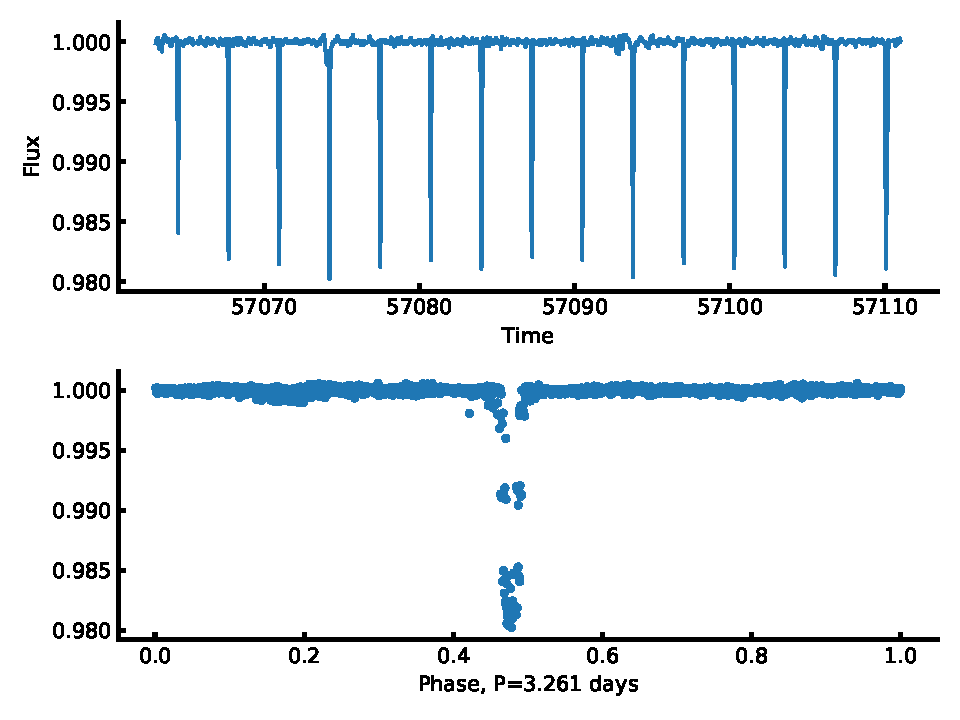
\includegraphics[width=1.0\linewidth]{figures/transitMethod.pdf}
    \caption{\emph{Upper plot}: The lightcurve of a star with an exoplanet transiting.
             \emph{Lower plot}: The phase curve of the above lightcurve.}
    \label{fig:transitMethod}
\end{figure}

As an exoplanet orbit a star, it might transit its host as seen from an observer here on Earth. This
signal might be detected if the star's brightness is being monitored as a periodic signal. The
decrease in brightness as the planet transit the star is directly related to ration between the
stellar radius $R_\ast$ and the planetary radius $R_p$:
\begin{align}
  k = \sqrt{\frac{R_p}{R_\ast}},  \label{eq:transit}
\end{align}
where $k$ is the depth of the transit compared to the total stellar brightness.

It is possible to obtain the radius of an exoplanet with this method. However, detailed analysis of
the phase curve of an exoplanet can reveal the surface temperature of the exoplanet. The transit
described above is also known as the primary transit. If it is possible to detect the secondary
transit, that is when the exoplanet goes behind the star as seen from Earth, the difference in light
(planet + star right before secondary transit compared to just star) gives the flux of the planet
and thus the surface temperature. This is a difficult task as secondary transits are intrinsic
faint.


\subsubsection{Radial velocity method}
\label{sec:rvmethod}

The radial velocity method is the indirect study of the motion of the host star using the Doppler
effect caused by an orbiting exoplanet. This together with the transit method described above is by
far the most successful methods to detect and characterise exoplanets. The periodic signal created
by the exoplanet on the host star depends on the mass ratio between the star $M_\ast$ and the planet
$M_p$:
\begin{align}
  K = \frac{\SI{28.4329}{km/s}}{\sqrt{1-e^2}} \frac{M_p\sin i}{\Mjup} \left( \frac{M_\ast+M_p}{M_\odot} \right)^{-2/3} \left(\frac{P}{\SI{1}{year}}\right)  \label{eq:rv}
\end{align}
where $K$ is the semi-amplitude of the sinusoidal, $e$ is the eccentricity, $i$ is the inclination,
$P$ is the orbital period, and $\Mjup$ is the mass of Jupiter. Since $M_\ast \gg M_p$, the term
$M_\ast+M_p\simeq M_\ast$ in order to simplify the equation. Often a circular orbit is assumed,
$e=0$. The sinusoidal motion of the star can be seen in \fref{fig:rvmethod} where both the time
series and the phase curve is presented for an exoplanet.

\begin{figure}[htpb!]
    \centering
    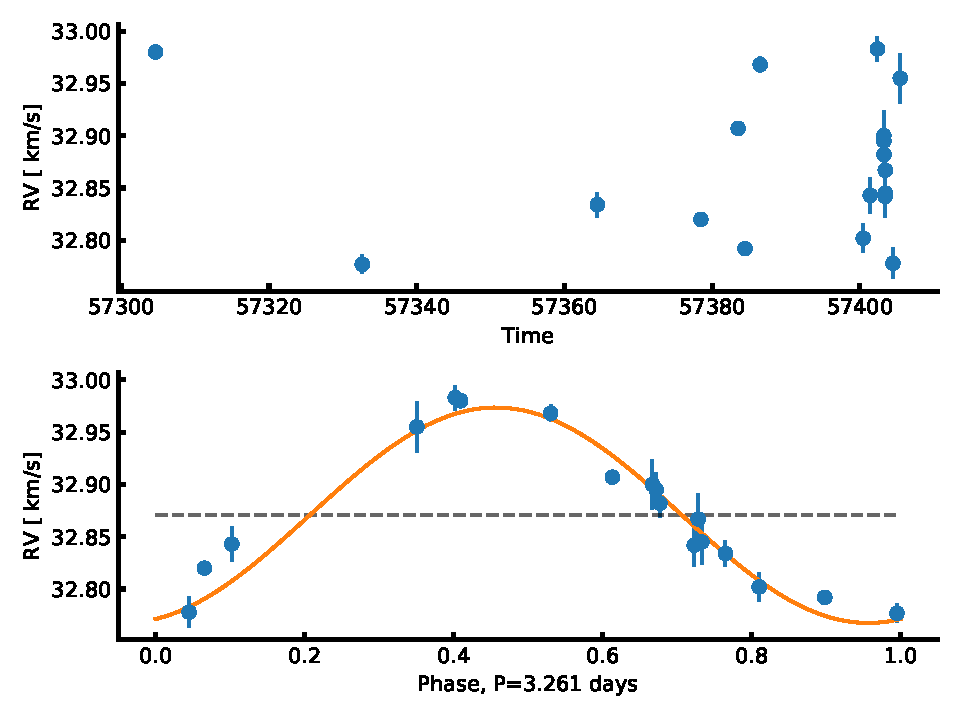
\includegraphics[width=1.0\linewidth]{figures/RVmethod.pdf}
    \caption{\emph{Upper panel}: RV time series of EPIC 9792 from the SOPHIE spectrograph.
             \emph{Lower panel}: Phase curve of the time series above, using the period of
             \SI{3.261}{days}.}
    \label{fig:rvmethod}
\end{figure}

In order to apply the radial velocity method for detecting exoplanets, it is necessary to collect
spectra, high resolution but often not high S/N, in order to cover most part of the phase of the
orbit. These spectra are often combined after the detection of the exoplanet, in order to increase
the S/N. This combined spectrum can then be used for characterising the host star.

This method is sensitive to close-in massive exoplanets, also known as hot Jupiters. In combination
with the above mentioned transit method, the mass and radius of an exoplanet can be derived, and
thus the bulk density which might give hints of the structure and composition of the exoplanet.


\subsubsection{Direct imaging}

Direct imaging is probably the easiest method to understand, however it is quite difficult to
actually use this technique. In its core, one has to carefully block the light of a star, and
directly imaging the exoplanets around it. However, it is extremely difficult to block the light of
the host star and find the reflected light of the exoplanet(s) in orbit.

This technique is sensitive to exoplanets which reflect a lot of light, i.e. a high albedo, and in
wide orbits as they are less contaminated by the residual starlight.

\subsubsection{Astrometry}

Using astrometry to detect exoplanets is very similar to the RV method described above in
\sref{sec:rvmethod}. Here an observer carefully detect the minute motion of a star caused by an
exoplanet. Unlike the RV method, this technique (astrometry) actually looks for changes in the
coordinates of the star. This technique has also been used to detect low luminosity stellar
companions as e.g. Sirius B.

This technique is sensitive to massive exoplanets as they cause a larger motion compared to lighter
companions.


\subsubsection{Transit timing variation}

This technique of detecting exoplanets is a highly indirect method of detecting exoplanets. Here an
observer first detect a transiting exoplanet as explained in \sref{sec:transitMethod}. Then
variations in the occurrence of mid-transit can be detected if a second non-transiting exoplanet
interact with the primary transiting exoplanet (planet-planet interaction). This interaction will
periodically course the mid-transit to happen ahead/behind of the time if only one exoplanet would
be present.

A careful analysis of the transit timing variations (TTV) can lead to the mass of the secondary
non-transiting exoplanet. However, its radius will be unknown. Most of these exoplanets pairs which
shows TTV are in an orbital resonant. This technique as well, is more sensitive to massive
exoplanets as they will induce a higher signal.


\subsubsection{Microlensing}

This technique is very exotic and not very useful, however since a few exoplanets have been
discovered by this technique it deserves a mentioning. The core theory in this technique is the
well-known General Relativity. Here an observer looks at a distant star (star A) as a star between
the observer and the distant star (star B) passes in front of the line of sight. Star B will act as
a microlens and increase the magnitude of star A. This increase of magnitude will reach its maximum
as the two stars are most aligned as seen from Earth.

To use this for detecting exoplanet, there will have to be an exoplanet orbiting star B. This act
like another lens, momentarily make a secondary increase in magnitude. The amount of increase in
magnitude is related to the mass of the exoplanet. The higher the mass, the higher the effect.

While this exotic technique is interesting and has proven successful, it is not very useful as it
only occurs once. The stars observed with this technique are often faint, thus making follow-up RV
detection very difficult if not impossible with the current instruments.


\subsection{Towards the Earth twin}

The above mentioned techniques will be used to find the Earth twin. Especially will the two first
techniques (transit and RV method) be the ones finding the smallest exoplanets as a wide range of
instruments are being developed dedicated for this\unfinished{Write about JWST, Espresso, NIRPS,
etc.}. Since the detection of the first exoplanet around a solar-type star by \citet{Mayor1995}, the
community has been able to detect lower mass exoplanets as seen in \fref{fig:exoplanetMass}.

\begin{figure}[htpb!]
    \centering
    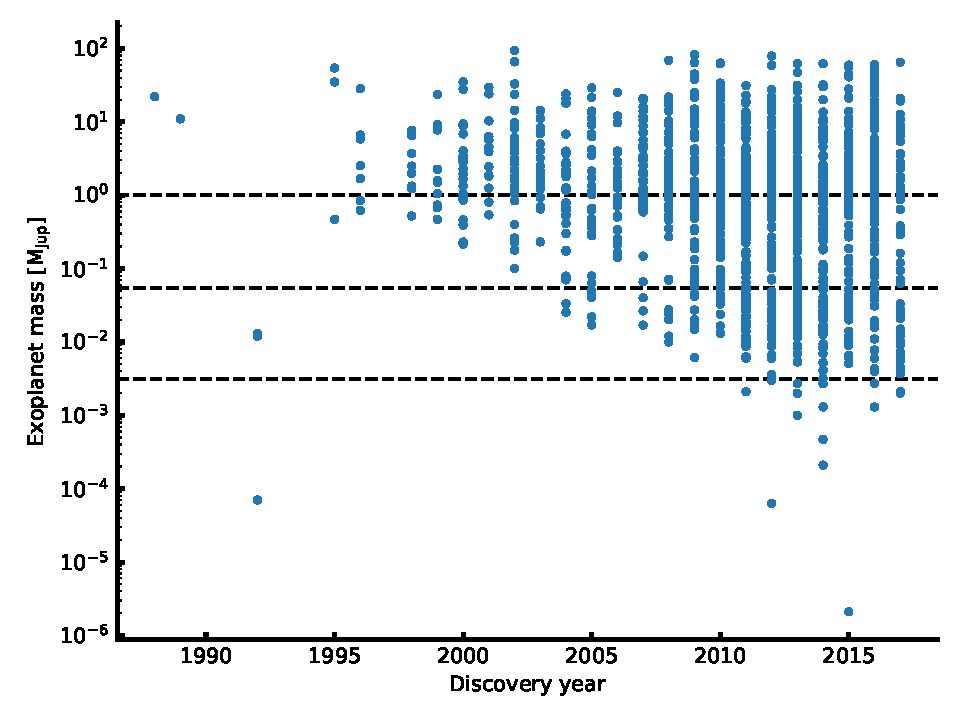
\includegraphics[width=0.8\linewidth]{figures/exoplanetMass.pdf}
    \caption{The mass of exoplanet since the detection of the first exoplanet until now. The
             horizontal lines are the mass of Jupiter (upper), Neptune (middle), and Earth (lower).}
    \label{fig:exoplanetMass}
\end{figure}

While the first many discoveries of exoplanets were the, at the time, exotic and strange hot Jupiter
like exoplanets in close orbits, the time have come to detect exoplanets with both lower mass and
wider orbits. It is crucial to have high precision instruments and long surveys to detect those
exoplanets. Missions as \emph{Kepler} and CoRoT have been excellent for this, since they have
focused on few fields of the sky for a long time.

The first place to look for Earth's twin is around a solar twin. However, since these stars are
quite hot, the habitable zone will also be far from the host star. Indeed, to detect a copy of our
own solar system we would need to detect the minute signature of an exoplanet in a \SI{1}{year}
orbit around its host star (a solar twin). If detected with the transit method, more than one
transit is needed, hence this will take at least two years, and probably even longer. The endeavour
to get the follow-up RV afterwards will also be extremely challenging with today's technology, and
only the next generation of spectrographs will be able to detect these signals.

Therefore, it is not a surprise that an effort have been towards detecting Earth-like planets around
less massive stars. These stars (M stars) are also colder, hence the habitable zone will be closer
to its host compared to the more massive and hotter stars. The nature have been kind, since it seems
that the M stars are prone to produce rocky planets rather than giant planets\reference{The ref. is
in the proposals}. The shorter period means that the surveys can be shorter for these planets.
Moreover, since they are smaller the signal from a transit will be easier to detect (see
\eref{eq:transit}). Similarly will the RV signal be larger for an Earth-like planet in the habitable
zone around an M star compared to a similar exoplanet around a G star. Both due to the lower period
and due to the lower mass of the host star (see \eref{eq:rv}).

While M stars seems to be the place to look for the Earth's twin, there are still some challenges to
tackle. Foremost is the detailed characterisation of the host star, which are particular troublesome
for these stars. This is something that will be focused on in the following section.




\section{Planet host stars}
\label{sec:planet_host_stars}

With the present diversity of exoplanets it becomes increasingly important to get an accurate and
precise characterisation of the exoplanets in order to study them in samples and on an individual
level. An accurate and precise characterisation can give us an idea whether the planet is rocky,
composed of water, gaseous, or some other more exotic combination. To characterise stars it is
common to use several different methods to learn about different aspects of a star. If the effective
temperature is needed, the most reliable comes from the analysis of a high resolution and high
signal-to-noise (S/N) spectrum. The same is used to identify chemical abundances of the photosphere
of the star, while methods like asteroseismology are used to determine the mass and radius of a
star, two parameters which are crucial to characterise the orbiting exoplanet.

Some of these methods are described in greater detail in \cref{cha:method}. These methods work best
together. In the example given above, the effective temperature is needed before asteroseismology
can be used to determine the mass and radius. These two methods goes extremely well together as the
most commonly used detection methods (transit and RV) will obtain the data needed. From the transit
method, one will obtain a lightcurve which can be used to detect the transits. If these are
carefully removed from the lightcurve, the residual might contain stellar oscillations used to
perform an asteroseismic analysis. Likewise will the spectra obtained from the RV method to
detect/confirm an exoplanet be used for the stellar characterising afterwards by combining them,
after shifting to a RV$=\SI{0}{km/s}$, to increase the S/N. This combined high S/N spectrum is ideal
for the spectral analysis of stars.

This tactic where spectroscopic analysis is used in conjunction with asteroseismology have proven
very successful\reference{Give ref here} for characterising an exoplanet system (host star and
exoplanet). However, it does have its limitations. It can be difficult to detect solar-like
oscillations as the stars get colder than the Sun. Especially have the community yet to detect any
solar-like oscillations in M dwarf stars\reference{Give ref here}. Other times the problem is on
spectroscopy. Many of the detected exoplanets are from the \emph{Kepler} mission, where many of the
host stars are very faint. While it is not impossible to make spectroscopic observations, it is
extremely time consuming. Therefore brighter targets are often prioritised, unless there is an
exceptional case.

With the search for the Earth twin around the small cool M dwarf stars, it is important to develop
reliable methods for the analysis of these stars. The tools for detecting the exoplanets are
currently more mature than the host star analysis. However, with the advance of NIR spectrographs
this is slowly changing. It is general believed that a NIR analysis is needed to characterise M
stars. The reason is simple that these stars are so intrinsic faint, that it is important to collect
as much flux as possible. This happens in the NIR. Moreover, for spectroscopic studies, the optical
spectrum of these stars are heavily contaminated by molecular absorption lines, which depress the
continuum. During spectroscopic topics, it is crucial to get the continuum placement correct. In the
NIR the continuum depression is less severe, however still challenging. This can clearly be seen in
\fref{fig:opticalVSnir} where the optical and NIR part of the spectrum for HD 79210, a K7 dwarf star
\citep{Kirkpatrick1991}, is plotted. The spectrum was obtained by CARMENES at the same time and have
therefore the same exposure time, hence roughly similar S/N. However, it is clear that the NIR
spectrum is far less contaminated by molecular lines.

\begin{figure}[htpb!]
    \centering
    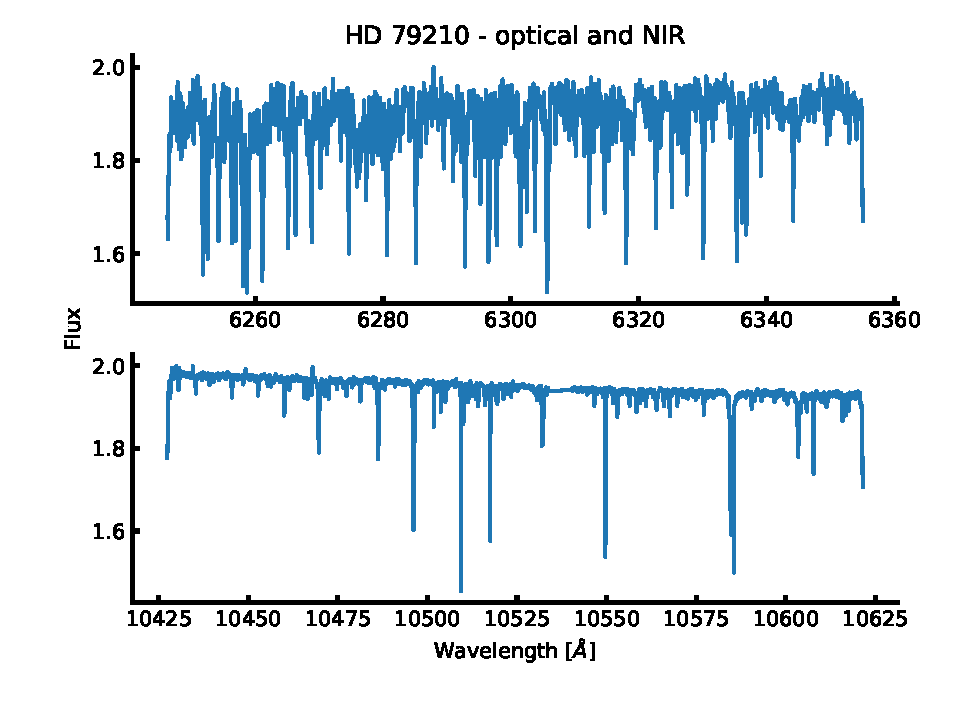
\includegraphics[width=1.0\linewidth]{figures/opticalVSnir.pdf}
    \caption{Comparison between a optical and NIR part of the spectrum of HD 79210 obtained by
             the CARMENES spectrograph. This clearly illustrate why NIR spectra are preferred over
             optical spectra for cool stars. HD 79210 is a K7 dwarf star.}
    \label{fig:opticalVSnir}
\end{figure}

The main goal of this thesis is to work towards a consistent deviation of stellar atmospheric
parameters for M stars. Before tackling the M stars, it is important to have a method that work
well for solar-like stars (FGK).



\section{Applications from knowing the stars}
\label{sec:stars_application}





\section{This thesis}
\label{sec:this_thesis}

%!TEX root = thesis.tex
\chapter{Theory of stellar spectroscopy in a nutshell}
\label{cha:theory}

\epigraph{``Begin at the beginning,'' the King said, very gravely, ``and go on till you come to the
          end: then stop.''}{Lewis Carroll, Alice in Wonderland}

To encompass all theory regarding stellar atmospheres is far beyond the scope of this thesis. Rather
the theory needed is presented below with highlights on the most important aspects.


\section{Stellar atmosphere}
\label{sec:stellar_atmosphere}

Much of this Section is inspired by \citet{Gray2006}. While all the figures here were made by the
author of this thesis, most of them can be found in \citet{Gray2006} as well.

Stellar atmospheres are rather complex. This is where the energy produced in the interior of the
stars \st{are} \hl{is} released. However, the atmosphere of a star is not transparent to all light,
and some of the light is absorbed or scattered in the atmosphere. In the case of absorption the
light will later be emitted in a random direction. This is seen as an absorption line in the stellar
spectrum. The different elements in the atmosphere is the reason for absorbing light at specific
wavelength. The strength of the absorption depends on the physical conditions in the atmosphere, the
effective temperature ($T_\mathrm{eff}$), the pressure/gravity ($\log g$), the \hl{chemical
abundances} \st{overall metallicity ($[\ion{Fe}/\ion{H}]$), the specific abundance of a given
element if different from the overall metallicity ($A$)}, and the atomic characteristics of the
transition coursing the absorption line.

\st{It is important to know} \hl{The strength of a line depends on} the fraction of atoms excited to
the $n$th energy level, $N_n$, \hl{on which the electron that produces the absorption is}. This
fraction is proportional to the statistical weight $g_n$ and the Boltzmann factor and is described
as:
\begin{align}
    \frac{N_n}{N} = \frac{g_n}{u(T)} 10^{-\theta\chi_n} \tag*{Boltzmann}\label{eq:boltzmann}
\end{align}
This equation is also called the Boltzmann equation. Here $N$ is the total number of atoms per unit
volume, $u(T)=\Sigma g_i e^{-\chi_i/kT}$ is the partition function, $k$ is Boltzmann's constant, $T$
is the temperature, and $\chi_n$ is the excitation potential for the lower energy level.

While atoms can get excited following Boltzmann's equation above, they can also get ionized. The
ionization ratio for a collision dominated gas (which is a good approximation for FGKM stars,
\hl{when assuming Local Thermodynamic Equilibrium, LTE}\footnote{\hl{LTE is obtained in stellar
atmospheres, when the length scale at which temperatures are changing are larger than the mean free
path. This is a good approximation for dwarf stars, where the mean free path is small, compared to
the larger mean free path in evolved stars, where LTE is no longer a good assumption.}}) is
described by the Saha equation. This equation relate the ratio of atoms in state $r$ to atoms in the
excited state above for the same element, $r+1$, in the following way:
\begin{align}
  \frac{N_{r+1}}{N_r} = \frac{1}{P_e} \frac{(2\pi m_e)^{3/2}(kT)^{5/2}}{h^3} \frac{2u_{r+1}(T)}{u_r(T)} e^{-I/kT} = \frac{\Phi(T)}{P_e} \tag*{Saha}\label{eq:saha}
\end{align}
here $m_e$ is the electron mass, $h$ is Planck's constant, $I$ is the ionization potential of the
neutral atom, and $\Phi(T)$ is all not related to the electron pressure, $P_e$.

The atomic lines are characterised by a few quantum mechanical descriptors.
\begin{itemize}
  \item \textbf{The wavelength}, $\lambda$, of an absorption (or emission) describes the energy
        difference between the two energy levels where the transition occurs.
  \item \textbf{The ionization state}, e.g. \ion{Fe}{I} describes iron in its atomic form, while
        \ion{Fe}{II} describes iron in its first ionized form.
  \item \textbf{The excitation potential}, $\chi$, \hl{is the excitation energy level of the lower
        state in the transition.} \st{This gives an idea how deep in the atmosphere a line
        is formed. If $\chi$ is high, then higher temperatures (i.e. higher random motion and more
        collisions between the atoms) is required for forming the absorption line. These higher
        temperatures are found deeper in the atmosphere.} \hl{A atomic line with a high $\chi$ is
        formed in the deeper layers of the atmosphere, since the higher temperatures there can
        excite the element. This is compared to the atomic lines with lower $\chi$ which are formed
        higher in the atmosphere at lower temperatures.}

  \item \textbf{The oscillator strength}, $\log \mathit{gf}$, is related to the atomic transition
        probability.
  \item \textbf{The damping coefficients}, $\Gamma$, is a natural damping (also known as radiation
        damping) caused by the uncertainty of lifetime in an energy level according to Heisenberg's
        uncertainty principle. This is related to a uncertainty in the energy level and thus a
        natural broadening is introduced.
\end{itemize}
These are essential to know from either theoretical calculations or experiments. The oscillator
strength is a quantity that is difficult to measure, and this is often changed when absorption lines
are matched with real observations of e.g. the Sun. This is a way of calibrating a line list and
will be described in detail in \sref{sec:linelist}.

It is important to mention that one of the main differences between absorption lines at different
wavelengths is the excitation potential. The energy levels of an atom gets denser packed as the
energy level increase as shown in \fref{fig:elevel} for hydrogen. For hydrogen the energy levels
$E_n$ follow the very simple formula from Bohr's atomic model, $E_n=\frac{\SI{-13.6}{eV}}{n^2}$,
where $n$ is the principal quantum number, and \SI{13.6}{eV} is the ionization energy for hydrogen,
i.e. the minimum amount of energy required to ionize hydrogen. The energy levels for heavier atoms
show a similar structure. The outer electron for a multi-electron atom is partially shielded from
the nucleus by the inner electrons, and thus does not experience the full charge $Z$ but rather an
effective charge $Z_\mathrm{eff}$, giving the expression
\begin{align}
  E_n = -hcR_\infty\frac{Z_\mathrm{eff}^2}{n^2},
\end{align}
where $h$ is Planck's constant, $c$ is the speed of light, and $R_\infty$ is Rydberg's constant.

With increasing $n$ the energy levels get closer, or in other words the photon required to excite an
electron from one energy level to a neighbouring state will get redder. These redder photons used
for exciting an atom are the absorption lines seen in the NIR. \st{However, the excitation to the
lower state is from thermal motion and not coursed by photons.} \hl{However, the excitation to the
lower state is related to the temperature and pressure according the} \ref{eq:boltzmann} \hl{and}
\ref{eq:saha} equations. Since tight energy levels require a highly excited lower state, the
temperature required here are similar high, which means that the NIR lines are typically formed in
the deeper layers of the atmosphere compared to absorption lines seen in the optical part of the
spectrum.

\begin{figure}[htpb!]
    \centering
    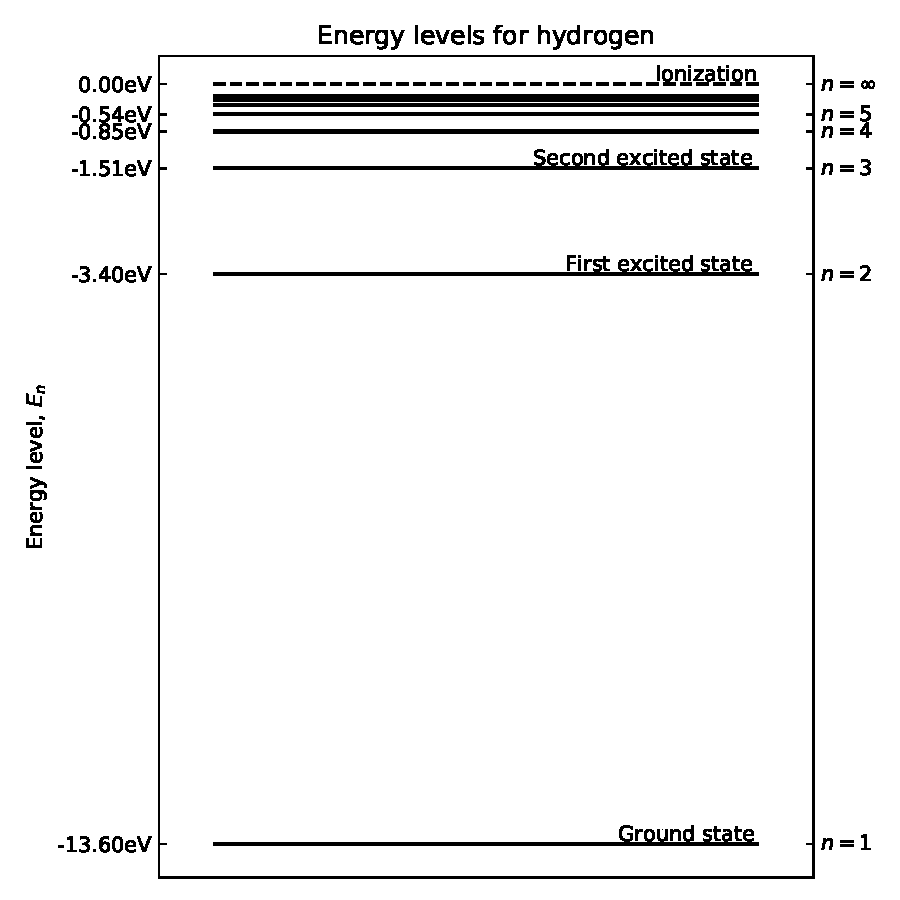
\includegraphics[width=0.85\linewidth]{figures/energyLevels.pdf}
    \caption{Energy levels for hydrogen, $E_n=\frac{\SI{-13.6}{eV}}{n^2}$.}
    \label{fig:elevel}
\end{figure}

The above discussed energy transitions are purely electronic, however there exists so called fine
structure transitions as well. This is due to the spin of the electron (or magnetic moment)
interacting with the orbital angular momentum of the electron. This leads to a splitting of the
absorption line. In atoms there also exists an even finer structure, commonly known as the hyperfine
structure. This structure arise due to the interaction between the magnetic field created by the
electrons and the nuclear spin. These splittings are important to consider for some transitions and
some atoms. For \ion{Fe}{} the hyperfine structure is not important since the net nuclear spin of
protons is 0 because there is an even number of protons, hence hyperfine structure is only important
for atoms with an odd number of protons. There are other splitting and shift for spectral absorption
lines like the Zeeman splitting coursed by an external magnetic field, and the Stark effect
splitting a line due to an external electric field. These two last effect are minor and will not be
discussed more, however it is worth noting that the Zeeman splitting can be used to measure the
strength of a magnetic field in a star if this is strong enough.



\subsection{Atmosphere models}
\label{sec:atmospheremodels}

In order to derive abundances or calculate a synthetic spectrum, two main things are needed: 1) An
atmosphere model, and 2) a radiative transfer code that solves the equations above. There are
different atmosphere models available. Throughout this thesis the ATLAS9 model atmosphere are used
\citep{Kurucz1993}. Other mention-able atmosphere models includes MARCS models \citep{Gustafson2008}
and the PHOENIX models \citep{Husser2013}. An atmosphere model is a description of the structure of
the atmosphere. This description has a number of quantities. The atmosphere model grids that are
available and used here have 72 layers. Each layer includes physical quantities such as temperature,
gas and electron pressure, \hl{and} the optical depth\st{, etc}. The models can be calculated on the
fly, but it is common practise because of computational reasons to pre-calculate a grid of
atmosphere models at certain $T_\mathrm{eff}$, $\log g$, and $[\ion{Fe}/\ion{H}]$. A specific
atmosphere model is then obtained from this grid by interpolating from nearest neighbours. The
interpolation code used throughout this work includes the four nearest neighbours in the
$T_\mathrm{eff}$-space, and the two nearest neighbours in both the $\log g$- and
$[\ion{Fe}/\ion{H}]$-space, in total $4\times2\times2=16$ atmosphere models to generate a single
interpolated atmosphere model.



\subsection{Radiative transfer code - \code{MOOG}}

There exists many different codes that solves the radiative transfer equations. In this thesis the
\code{MOOG} code is used by \citet{Sneden1973} \hl{which assumes LTE}. This code has different
drivers, only some are used here.
\begin{itemize}
  \item Derive a theoretical equivalent width (see \sref{sec:EW} for details) for a given star, i.e.
        atmosphere model with a given set of atmospheric parameters.
  \item Derive line abundance from a measured equivalent width for a given model atmosphere.
  \item Calculate a synthetic spectrum for a given model atmosphere and atomic line list.
  \item Calculate the curve-of-growth for an atomic line.
\end{itemize}
There exists other drivers as well, but these are the ones used here. Some only for visualising the
figures below.



\subsection{The equivalent width}
\label{sec:EW}

Measuring the equivalent width (EW) of spectral lines are important for some analysis of stellar
spectra. The EW is a measure of the strength of the line, and dependent on the atmospheric
conditions in where the spectral line is formed, such as $T_\mathrm{eff}$, $\log g$,
$[\ion{Fe}/\ion{H}]$, and $\xi_\mathrm{micro}$.

\begin{figure}[htpb!]
    \centering
    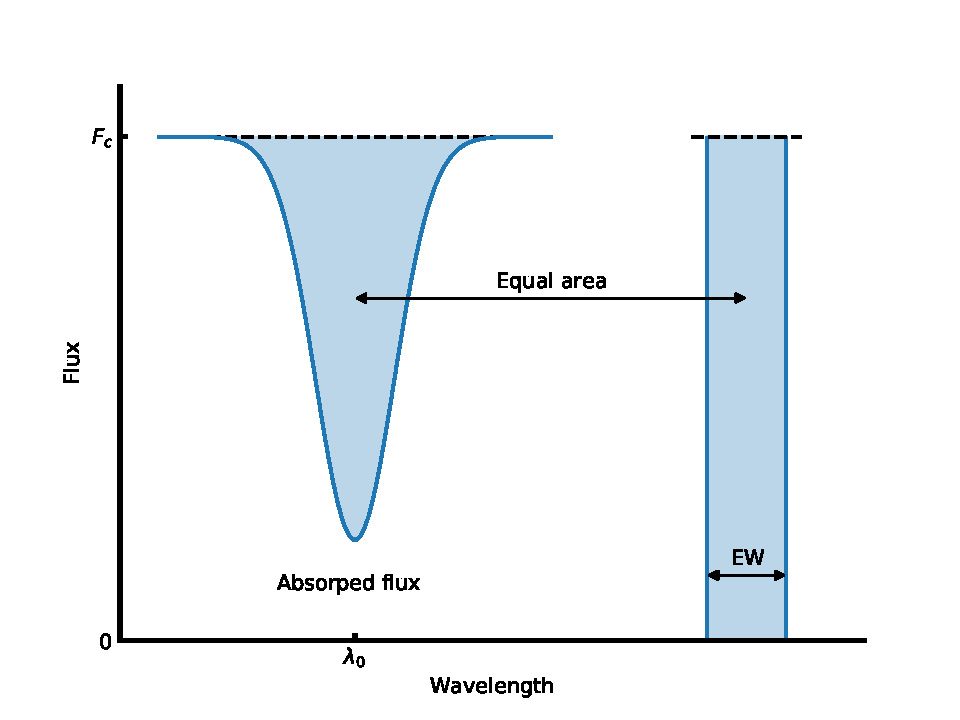
\includegraphics[width=0.85\linewidth]{figures/ewTheoretical.pdf}
    \caption{An absorption line centred at $\lambda_0$ normalised at the flux level $F_c$. The area
             of the absorption line to the left is equal to the blue shaded area in the rectangle to
             the right with width EW.}
    \label{fig:ewTheoretical}
\end{figure}

The EW is mathematically described as integrating over the entire line, and assign this area to a
rectangle from 0 to the continuum flux ($F_c$) with the width, EW. This is illustrated in
\fref{fig:ewTheoretical} and the equation below: \begin{align} EW = \int_{0}^{\infty}
\frac{F_c-F(\lambda)}{F_c} d\lambda, \end{align} where $\lambda$ is the wavelength. This is integral
is assuming there is only one single line, hence the integral is over all wavelength. In practice
the integral is calculated in small windows around a spectral line. See \sref{sec:measureEW} for
more details on how this is performed in practice. The unit of the EW is the same as the wavelength
used. Throughout this thesis we will use \AA{}ngstr\"{o}m ($\SI{1}{\angstrom}=\SI{0.1}{nm}$) for the
wavelength, and \si{m\angstrom} for the EW.


\subsubsection{Temperature dependence}

\hl{As mentioned above, the theory presented here is the bare minimum. For the full derivations of
the equations presented below see Chapter 13 in} \citet{Gray2006}.

As mentioned above the EW depends on the atmospheric parameters. \st{The dependence on
$T_\mathrm{eff}$ is the strongest dependence.} At low $T_\mathrm{eff}$ neutral elements, say
\ion{Fe}{I}, are the strongest lines as the number of ionized atoms are too small to contribute
significantly to the EW. This is the result the Saha equation. As $T_\mathrm{eff}$ increases
\ion{Fe}{I} is converted into ionized \ion{Fe}{II}. Slowly, as the number of \ion{Fe}{I} decreases
so does the EW, and likewise as the number of \ion{Fe}{II} increases so does the EW. This goes on
until second ionized atoms, \ion{Fe}{III}, are formed and the same situation arise again. This is
illustrated in \fref{fig:ewTeff} where the EW of two iron lines, one neutral and one ionized, are
plotted against $T_\mathrm{eff}$. These two lines have similar EW in the Sun:
$\SI{46.2}{m\angstrom}$ and $\SI{53.9}{m\angstrom}$ for the \ion{Fe}{I} and \ion{Fe}{II} line
respectively.

\hl{This can be explained with four simple cases:}
\begin{itemize}
  \item[Case 1] \hl{Weak line of a neutral species (e.g} \ion{Fe}{I}\hl{) with the element mostly neutral}
  \item[Case 2] \hl{Weak line of a neutral species with the element mostly ionized}
  \item[Case 3] \hl{Weak line of an ion species (e.g} \ion{Fe}{II}\hl{) with the element mostly neutral}
  \item[Case 4] \hl{Weak line of an ion species with the element mostly ionized}
\end{itemize}
\hl{The behaviour of the line strength $R$ is shown in the equations below for the four different
cases}
\begin{align}
  \frac{1}{R}\dd{R}{T} &= \frac{2.5}{T} + \frac{\chi+0.75}{kT^2}-\Omega  \tag*{Case 1} \\
  \frac{1}{R}\dd{R}{T} &= \frac{\chi+0.75-I}{kT^2}                       \tag*{Case 2} \\
  \frac{1}{R}\dd{R}{T} &= \frac{5}{T} + \frac{\chi+0.75+I}{kT^2}-2\Omega \tag*{Case 3} \\
  \frac{1}{R}\dd{R}{T} &= \frac{2.5}{T} + \frac{\chi+0.75}{kT^2}-\Omega, \tag*{Case 4}
\end{align}
\hl{where $\chi$ is the excitation potential, $I$ is the ionization energy, and $\Omega$ can be
considered a constant as it mildly depends on pressure. The four cases are also shown in}
\fref{fig:ewTeff}.

\begin{figure}[htpb!]
    \centering
    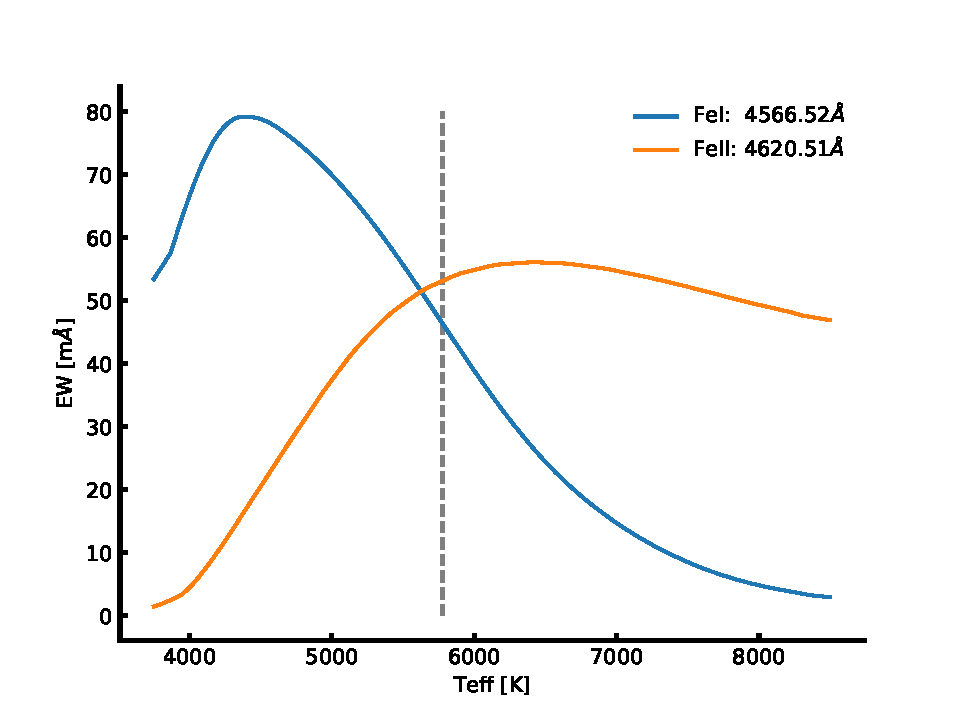
\includegraphics[width=0.85\linewidth]{figures/ewTeff.pdf}
    \caption{The EW for a \ion{Fe}{I} and \ion{Fe}{II} line with increasing $T_\mathrm{eff}$. The
             two lines have similar EW in the Sun and are found in the optical part of the spectrum.
             The vertical line show the solar $T_\mathrm{eff}$.}
    \label{fig:ewTeff}
\end{figure}


\subsubsection{Pressure dependence}

Pressure dependence in the stellar atmosphere can be related to the gravity dependence. There are
many ways to measure the pressure, and thus the gravity which is what is ultimately the goal with
the measurement of $\log g$. Below are listed some of the most common methods to measure $\log g$
from spectroscopy.

\begin{itemize}
  \item Continuum: The Balmer jump is the only continuum feature sensitive enough to estimate the
        $\log g$.
  \item Hydrogen lines: Hydrogen profiles are pressure \hl{and temperature} sensitive and can
        therefore be used to estimate $\log g$. However, the gravity dependence rapidly diminishes
        for temperatures above $\SI{10\,000}{K}$.
  \item Other strong lines: There exists other strong lines with pressure-broadened wings such as
        the \ion{Ca}{II} H and K lines. These are better for cooler stars than the hydrogen lines
        described above.
  \item Weak lines: By comparing two stages of ionization for the same element it is possible to
        obtain $\log g$ using weaker or modestly strong lines.
\end{itemize}
In this thesis weak lines are used to measure $\log g$. More specifically a comparison between
\ion{Fe}{I} and \ion{Fe}{II} lines are used. For FGK stars, as the atmosphere contracts (i.e. $\log
g$ increases) the pressure likewise increases, which in turn means that both the gas pressure,
$P_g$, and electron pressure, $P_e$, increases. Since hydrogen is the main electron contributor, but
not fully ionized for these stars, the electron pressure is much smaller that the gas pressure. The
gas pressure follow a simply empirical approximation with gravity:
\begin{align}
  P_g \approx \mathrm{constant}\, g^{2/3},
\end{align}
where $g$ is the gravity. The electron pressure is given by
\begin{align}
  P_e \approx \mathrm{constant}\, g^{1/3}.
\end{align}

There are three cases for which a line show dependence on gravity, when considering only weak lines:
\begin{enumerate}
  \item A weak line formed by any ion or atom, where most of the element is in the next higher ionized state.
  \item A weak line formed by any ion or atom, where most of the element is in the same ionized state.
  \item A weak line formed by any ion, where most of the element is in the next lower ionized state.
\end{enumerate}

Using the Saha equation for case 1, it is important to note that the number of the atoms in the
highest state is roughly equal to the total number of atoms of that element, $N_{r+1}\approx N$.
Hence
\begin{align}
  N_r \approx \mathrm{constant}\,\, P_e
\end{align}
which means that the line absorption coefficient is
\begin{align}
  l_\nu \approx \mathrm{constant}\,\, N_r \approx \mathrm{constant}\,\, P_e.
\end{align}
The strength of a weak line, $R$, is proportional to the ratio of the line to the continuous
absorption coefficient, $\kappa_\nu$
\begin{align}
  R = \frac{F_c-F_\lambda}{F_c} = \mathrm{constant}\,\, \frac{l_\nu}{\kappa_\nu}.
\end{align}
When negative hydrogen dominates $\kappa_\nu$ which is the case here it is proportional to the
electron pressure, $\kappa_\nu\propto P_e$ which means the line strength is not proportional to
electron pressure:
\begin{align}
  R = \frac{l_\nu}{\kappa_\nu} \approx \mathrm{constant}.
\end{align}

For case 2, the approach is the same, here $N_r\approx N_{r+1}\approx N= \mathrm{constant}$. This
leads to $l_\nu\approx\mathrm{constant}$, eventually giving
\begin{align}
  R=\frac{l_\nu}{\kappa_\nu} \approx \frac{\mathrm{constant}}{P_e} \approx \mathrm{constant}\,\, g^{-1/3}.
\end{align}
Only the first two cases are relevant for solar-type stars used in this thesis, and the relation for
the third case will be omitted.

In \fref{fig:ewGravity} is shown how the \ion{Fe}{II} line used previously change with $\log g$. The
curve of growth is shown in the upper panel, while a synthetic spectrum for each $\log g$ is
presented in the lower left panel. It is clear that the ionized line is sensitive to $\log g$ as
shown in the lower right panel, where the correlation between the abundance and $\log g$ is 0.40.
This is expected as can be seen in \citet[][Table 16.1]{Gray2006}. There is used $\delta\log
A/\delta\log g$ as an indicator, and for neutral elements the correlation is much weaker. It is
important to note that the correlation does change with $T_\mathrm{eff}$ and the element used.

\begin{figure}[htpb!]
    \centering
    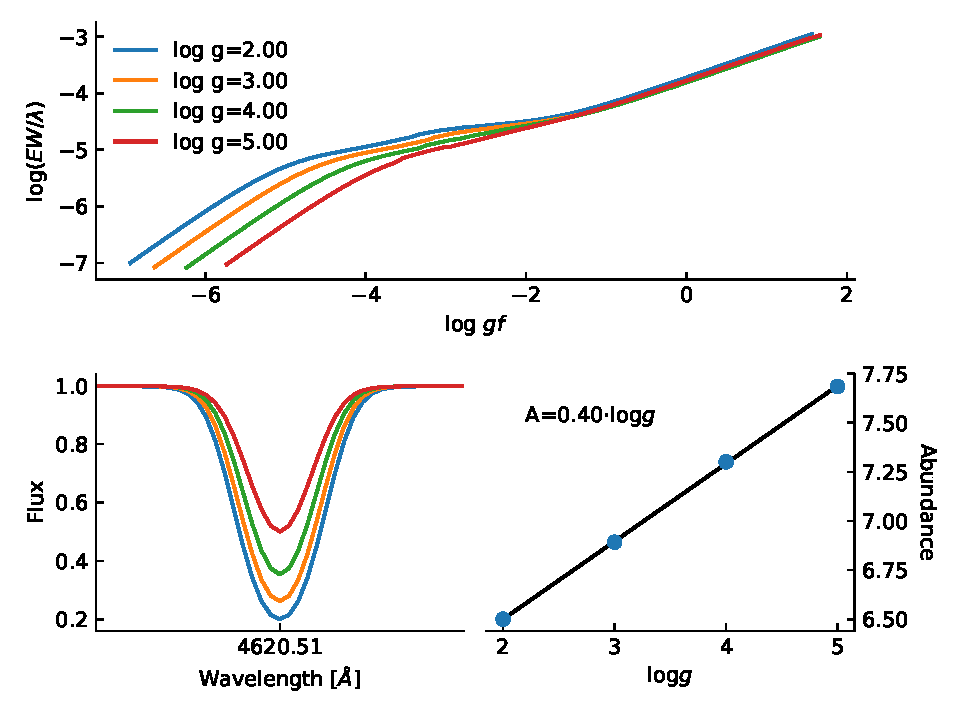
\includegraphics[width=0.85\linewidth]{figures/ewGravity.pdf}
    \caption{\emph{Upper panel}: Curve of growth for same \ion{Fe}{II} used in \fref{fig:ewTeff} for
                                 four different $\log g$ values. Here it is the weak lines mostly
                                 affected by the change in $\log g$.
             \emph{Lower left panel}: Synthetic spectra of the same line. The colour scale is the
                                      same.
             \emph{Lower right}: The abundance for the line at different $\log g$. A strong
                                 correlation (0.40) is seen.}
    \label{fig:ewGravity}
\end{figure}




\subsubsection{Abundance dependence}

The abundance of a given element obviously has an effect on the EW. The more abundant an element is,
the more photons can be absorbed thus increasing the EW. However, the relationship is not strictly
linear. For weak lines (GIVE RANGE) EW is approximately linear with the abundance, however it reach
a plateau where the core of the line saturates. In this regime the EW only increases slowly, until
the absorption ``spills'' into the wings and the increase is again linear. However, for these strong
lines the profile is no longer Gaussian. The curve of growth for the same \ion{Fe}{I} line used in
\fref{fig:ewTeff} is shown in \fref{fig:cog}. Instead of EW it is common to use the reduced EW,
$\log (EW/\lambda)$\footnote{The reduced EW is useful since it normalises Doppler-dependent
phenomena, such as microturbulence and thermal broadening.}, which we will use more later.
\st{Instead of the abundance of a line, the oscillator strength, $\log \mathit{gf}$, is used.}

\begin{figure}[htpb!]
    \centering
    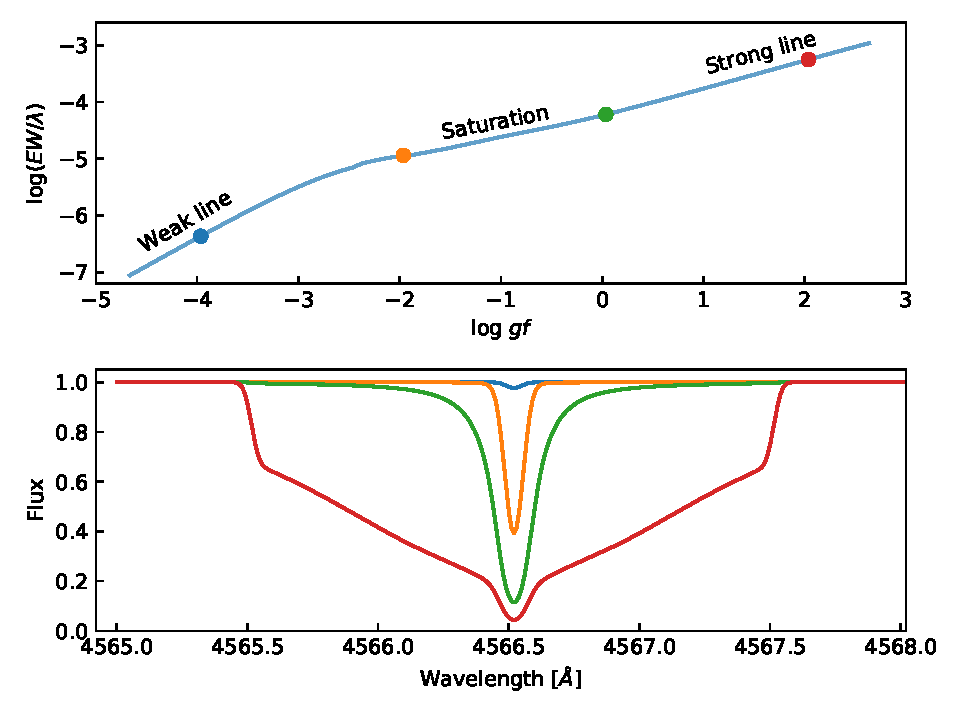
\includegraphics[width=0.85\linewidth]{figures/cog.pdf}
    \caption{\emph{Upper panel:} Curve of growth of the same \ion{Fe}{I} line as used in
                                 \fref{fig:ewTeff}. Four points are marked which is shown in the
             \emph{lower panel} as a synthetic spectral line. The RW (proxy for EW) is clearly
                                increasing with \hl{abundance} \st{$\log \mathit{gf}$ (proxy for abundance).}}
    \label{fig:cog}
\end{figure}


\subsubsection{Microturbulence}

Small-scale motion, that is motion of material at length scales small compared to the unit optical
depth, are called microturbulence, $\xi_\mathrm{micro}$. This is not to be confused with
macroturbulence, which is motion of material at scales larger than the unit optical depth. The
latter is associated with granulation and will not be discussed further in this thesis.
$\xi_\mathrm{micro}$ comes into play when looking at the curve of growth for saturated lines (i.e.
between green and red points in \fref{fig:cog}). If no $\xi_\mathrm{micro}$ is assumed, then the
measured abundance is higher than predicted by models based on thermal and damping broadening alone.
In \fref{fig:cog_vt} is shown three curves of growth with $\xi_\mathrm{micro}={\SI{0.5}{km/s},
\SI{2.5}{km/s}, \SI{5.0}{km/s}}$. As $\xi_\mathrm{micro}$ increases, so does the EW and hence the
abundance.

\begin{figure}[htpb!]
    \centering
    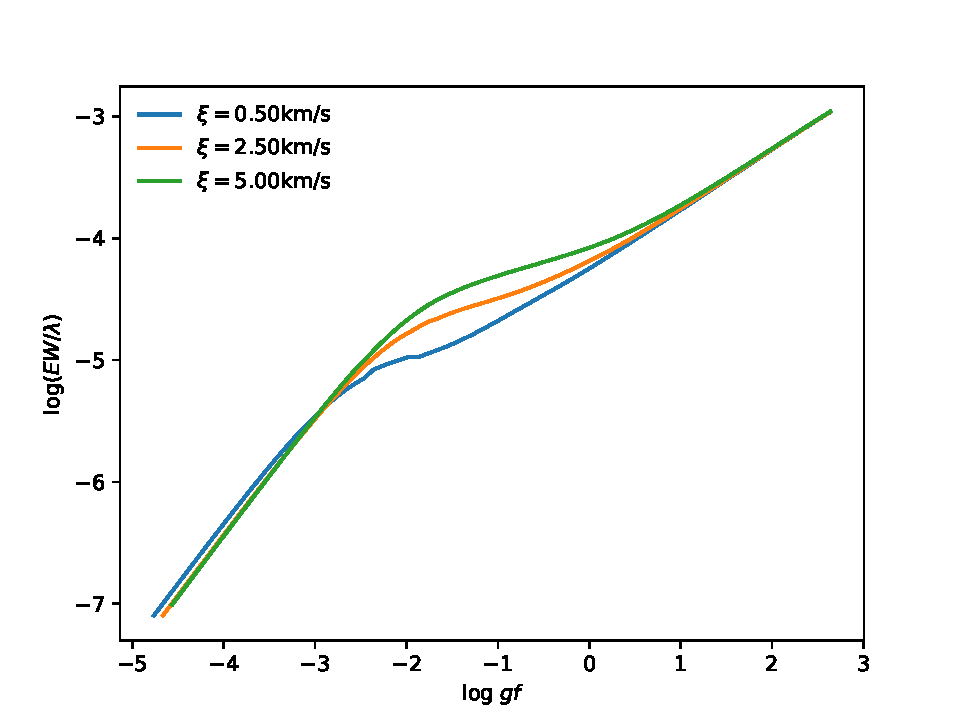
\includegraphics[width=0.85\linewidth]{figures/cog_vt.pdf}
    \caption{Curve of growth for three different values of $\xi_\mathrm{micro}$. The EW is
             increasing with increasing $\xi_\mathrm{micro}$.}
    \label{fig:cog_vt}
\end{figure}

The broadening of an absorption line measured by the shift in wavelength, $\Delta\lambda$, when
$\xi_\mathrm{micro}$ is included is defined as:
\begin{align}
  \Delta\lambda = \frac{\lambda_0}{c} \sqrt{\frac{2kT}{m} + \xi_\mathrm{micro}^2},
\end{align}
where $c$ is the speed of light, $\lambda_0$ is the rest wavelength of the given line, $k$ is
Boltzmann's constant, $T$ is the temperature, and $m$ is the mass of the atom. Setting
$\xi_\mathrm{micro}=\SI{0}{km/s}$, we end up with thermal broadening.


\section{Line list and atomic data}
\label{sec:linelist}

As mentioned above, the atomic data of the absorption lines are required. These data can be found in
a database such as \emph{The Vienna Atomic Line Data Base} (VALD) \citep{VALD1,VALD2}. For compiling
a usable iron line list, all theoretical transitions in a given wavelength range are requested from
VALD. In the near-infrared (NIR), YJHK bands, there are several thousands of theoretical
transitions.

In this thesis the EWs are measured (see \sref{sec:measureEW}) for all these lines using a solar
spectrum \citep[][is used here]{Hinkle1995}. Here there are four possible outcomes. 1) A line can
not be measured and is thus discarded, 2) the EW of the line is weak (below \SI{5}{m\angstrom}) to
be reliable, 3) the EW of the line is too strong (above \SI{150}{m\angstrom}) and the line show
non-linear behaviour in the curve-of-growth (see \fref{fig:cog}), or 4) the EW of the line is
between the two limits and is then added to the final line list.

After removing lines which EW is outside the range of EW mentioned above, it is good practise to
have a visual inspection. Here one should look for severe line blending with other absorption lines
which might prove problematic and unreliable measurements of the EW. If the reference spectrum used,
here for the Sun, is not corrected for telluric lines, it is also a good idea to remove lines which
exists amidst forest of telluric lines, as these absorption lines might fall on the telluric lines,
if the star observed has a different radial velocity (RV).

When blended lines and otherwise lines which shows strange features (can be in a forest of telluric
lines), the last step is to calibrate the atomic data. As mentioned above, this is done by changing
the $\log \mathit{gf}$ value for a given line, until it has the desired determined abundance. In
this case, an iron line should have the abundance of 7.47 using the values from
\citet{Gonzalez2000}, when using a solar atmosphere model. There is a simple anti-correlation
between the determined abundance from the measured EW and the $\log \mathit{gf}$, so a simple
bisector minimization can be used to find the best $\log \mathit{gf}$. It is important to calibrate
the $\log \mathit{gf}$ when changing the version of \code{MOOG} (or if other radiative transfer
codes are used), the atmosphere model and version of those, and even the interpolation of the
atmosphere models. These changes in $\log \mathit{gf}$ should be minor compared to the change from
the VALD database and those we arrive at when calibrated for the Sun.



\section{Spectrographs}
\label{sec:spectrographs}
\unfinished{Not sure what the purpose is of this, but it can be relevant somewhere.}

This chapter will be focused on some of the available spectrographs for deriving stellar atmospheric
parameters using the method described in \sref{sec:parameters}. For this we need a spectrum of both
high resolution and high signal-to-noise ratio, S/N, which combined will be called a high quality
spectrum. In order to get reliable results, a spectral resolution of at least
$R=\frac{\lambda}{\Delta\lambda}=25\,000$ is needed. A $S/N\approx 100$ is at least needed to obtain
the parameters. These are approximately values since it can vary across different spectral classes,
e.g. it is often relatively easy to obtain parameters of a solar-twin while it gets increasingly
difficult as especially $T_\mathrm{eff}$ diverges in either direction from the solar value.
Naturally the higher quality the spectrum is (both resolution and S/N), the better the results will
be obtained. It is common practise to increase the S/N for a spectrum by co-adding a sample of lower
S/N spectra of the same star from the same spectrograph. This is often used if the star of interest
is so dim that it takes several observations to reach a sufficient high S/N. Another case is when
spectra have been obtained from the archive. The scientific goal can be very different, e.g.
obtaining radial velocities (RV) where a much lower S/N is needed, however here numerous spectra are
needed. It is common to search for exoplanets with the RV detection method, where multiple spectra
are obtained, and the stellar parameters are then obtained after co-adding the multiple spectra. It
is of course important to put the spectra on a common RV, usually at \SI{0}{km/s}.

Spectrographs work in different wavelength regions. The most used region is the optical part of the
spectrum, which is also ideal for studying FGK stars with relative low line blending and low
telluric contamination. In the recent years there has been an increase of NIR spectrographs. These
will mainly be used to study the distant Universe, i.e. at high red-shifts, and cool objects in our
own galaxy. Especially interesting are the M stars which consist of around 70\% of all stars in our
galaxy \citep{Bochanski2010}. These stars are intrinsic dim because of their low $T_\mathrm{eff}$,
ranging from \SIrange{2200}{3500}{K}, hence most of their light emitted will be in the NIR. It is
advantageous to collect as much light as possible from these dim stars, since reaching a similar S/N
in the optical would be more time expensive. The cool M stars have more molecules in the atmosphere
than their hotter counterparts. This can be seen in the spectrum, where molecular lines greatly
depress the continuum, making EW measurements difficult. This continuum depression is much larger in
the optical than the NIR, giving another motivation for studying stars in this wavelength region.

%!TEX root = thesis.tex

\chapter{Deriving stellar parameters}
\label{cha:method}


\section{Different methods for atmospheric parameters}

\subsection{IRFM}

\subsection{Photometry}

\subsection{Spectroscopy}


\section{Other stellar parameters}

\subsection{Asteroseismology}


\section{\FASMA}
\label{sec:parameters}

In this section, the process from a spectrum to atmospheric parameters will be
explained in details. There are two classic methods, synthetic fitting and
curve-of-growth analysis.

The synthetic fitting method is in simple terms a comparison between the
observed spectrum and a synthetic spectrum, which is either calculated on the
fly like SME \citep{Valenti1996}, or using a pre-calculated grid. By analysing
the $\chi^2$ the synthetic spectrum that best match the observed spectrum can be
found. This technique works for all ranges of spectral resolutions and can work
for many rotational profiles as well \citep[see e.g.][]{Tsantaki2017}. However,
this method is often time-consuming compared to the curve-of-growth analysis.

Here the curve-of-growth analysis will be explained in detail. In particular
Fast Analysis of Spectra Made Automatically (\FASMA) which was developed during
this thesis.


\subsection{Ingredients}

\FASMA is written in the Python programming language and glue together other
software and models necessary for obtaining stellar atmospheric parameters from
high quality spectra. These software and models are described in greater detail
below. In short, the curve-of-growth analysis require measured EWs where the
latest version of ARES is used \citep{Sousa2015a}. These EWs are used to derive
line abundances using model atmosphere like the ATLAS9 \citep{Kurucz1993}, MARCS
models \citep{Gustafson2008}, and PHOENIX models \citep{Husser2013} to mention
the most popular for this analysis. Note that the PHOENIX models are relative
new and not as widely used yet. In tandem with model atmospheres a radiative
transfer code is also needed. \FASMA uses MOOG \citep{Sneden1973} for this,
however there are other codes available, e.g. \unfinished{Mention some other
codes here}. The model atmosphere usually comes in a pre-calculated grid in the
$\{T_\mathrm{eff},\,\log g,\,[\ion{Fe}/\ion{H}]\}$ parameter space. These are
interpolated in order to access the requested combination of parameters. Last,
\FASMA consist of a minimization routine which looks for the right parameters
given a spectrum.




\subsection{Interpolation of atmosphere models}

\FASMA has access to both ATLAS9 models by \citet{Kurucz1993} and MARCS models by
\citet{Gustafson2008}, both are in a pre-calculated grid as described above. Let
this grid be described by $\{T_\mathrm{eff,g},\,\log
g_g,\,[\ion{Fe}/\ion{H}]_g\}$, where $g$ is one of the grid points.
\unfinished{Make a table or plot describing the grid}. The requested value will
be $\{T_\mathrm{eff,r},\,\log g_r,\,[\ion{Fe}/\ion{H}]_r\}$. The task is now to
find the surrounding grid points in the parameter space of the requested
parameters. For $\log g$ and $[\ion{Fe}/\ion{H}]$ two neighbouring grid point
are used, and for $T_\mathrm{eff}$ four surrounding grid point are used, in
total $4\times2\times2=16$ model atmospheres for the interpolation. \FASMA use
the four surrounding grid points for $T_\mathrm{eff}$ instead of two, since the
model atmosphere changes most with $T_\mathrm{eff}$. This is common in other
interpolations\reference{Give ref here} as well.

When the 16 model atmosphere have been located, the interpolation goes through
each layer of the model atmosphere, where there typical are 72 layers, and each
column of which there are six. The columns are described in
\sref{sec:atmospheremodels}. The interpolation are done using the
\code{griddata} function from
\code{SciPy}\footnote{\url{https://scipy.org/}}. The interpolation is linear
in the parameter space. After the interpolation, the result is saved to a file
in the format expected by MOOG.





\subsection{Wrapper for ARES}
\label{sec:measureEW}

There are two ways to measure the EW of an absorption line, manual or automatic.
Both of these methods are used here. There are advantages and disadvantages for
both method. For the manual, an advantage is that we can inspect the lines and
try to measure lines in different ways (which is useful if it is blended).
Disadvantages are that it is very time consuming, and it is prone to errors, as
a measurement might change drastically by the eyes measuring it. Even for the
same person, the measurement can change. By mentioning the advantages and
disadvantages of the manual method, it should be clear that the advantages and
disadvantages of the automatic method is the opposite of those. Especially the
time to measure the lines is order of magnitudes faster, which is crucial when
dealing with more than a handful of spectra.

When a line is measurement by hand (manual) it is done using the splot command
in IRAF. Here the deblending mode is used whenever necessary. It is often
necessary to fit one spectral lines with several Gaussian's, as neighbouring
lines might contaminate the line of interest slightly.

When a line is measurement automatically it is done with ARES
\citep{Sousa2007,Sousa2015a}. When using ARES it is important to use a correct
value of the rejt parameter. This parameter is used for placing the continuum
level, and is thus directly related to the final measurement EW. It is difficult
to get this parameter right, however the newest version of ARES has the option
to analyse a few absorption free regions and measure the S/N. The rejt is then
calculated as:
\begin{align*}
  rejt = 1 - \frac{1}{S/N}.
\end{align*}

As all, or as many as possible, the lines in the line list have measured EWs,
the next step in determining the atmospheric parameters is to determine the
abundance for each line and imposing excitation and ionization balance.


\subsection{Minimization}

With the measured EWs for all the lines in the line list, we choose an
atmosphere model to determine the abundances. If there is no prior knowledge of
the star it is common simple choose a solar atmosphere model as a starting
point. Next the correlation between the abundances and the reduced EWs, and the
abundances and the excitation potential is calculated. If there is a correlation
it means the atmosphere model used is wrong. Moreover, we also have to check if
the mean abundance of \ion{Fe}{I} and \ion{Fe}{II} lines are equal, and last if
mean abundance of the \ion{Fe}{I} lines is equal to the input
$[\ion{Fe}/\ion{H}]$ of the atmosphere model\footnote{We use \ion{Fe}{I} instead
of \ion{Fe}{II} lines for this, since they are more numerous.}. If one of these
four criteria does not pass, then the atmosphere model is wrong, and we have to
search for a new one. A common way to do this, is by combining the indicators
into a scalar value:
\begin{align}
  f(\{T_\mathrm{eff}, \log g, [Fe/H], \xi_\mathrm{micro}\}) &= \sqrt{a_\mathrm{EP}^2 + a_\mathrm{RW}^2 + \Delta\ion{Fe}{}^2},
\end{align}
where $a_\mathrm{EP}$ is the correlation between abundances and excitation
potential, $a_\mathrm{RW}$ is the correlation between abundances and reduced EW,
and $\Delta\ion{Fe}{}$ is the difference between the mean abundances of
\ion{Fe}{I} and \ion{Fe}{II}. This scalar function can be minimized using
standard minimization procedures as the simplex downhill among others. However,
there is another approach that takes into the account the information stored in
these indicators. For example, if $a_\mathrm{EP}$ is positive it means
$T_\mathrm{eff}$ has to be increased by an amount correlated by the numerical
value of $a_\mathrm{EP}$. In the same way, a non-zero $a_\mathrm{RW}$ means
$\xi_\mathrm{micro}$ has to be changed, and $\Delta\ion{Fe}{}$ is an indicator
for $\log g$. In the end it is a vector function being minimized which are more
difficult, however we are not minimizing this using standard mathematical
methods, but rather using the physical knowledge. This minimization is useless
for anything else, but it is excellent for this.
The vector function has the form:
\begin{align}
    f(\{T_\mathrm{eff}, \log g, [Fe/H], \xi_\mathrm{micro}\}) = \{a_\mathrm{EP}, a_\mathrm{RW}, \Delta\ion{Fe}, \ion{Fe}{I}\}.
\end{align}

In each iteration where convergence is not reached, the input metallicity is
changed to that of the mean output metallicity using the \ion{Fe}{I} lines. The
minimization is depicted in \fref{fig:minimization}. This minimization is
written in the Python programming language and is also a wrapper around both
ARES and MOOG. The entire package is called \FASMA\footnote{Greek for spectrum}
\citep{Andreasen2017a, Tsantaki2017}. \FASMA is able to fix one or all of the
four atmospheric parameters, and when it reach convergence it checks if there
are any outliers in the abundances. These will be removed, either all at once,
all iteratively, meaning that after removing the outliers the minimization is
restarted at the previous best parameters, and this process is continued until
there can be removed no other outliers, or last is removing one outlier
iteratively. An optical line list like the ones by
\citet{Sousa2008a,Tsantaki2013} have been tested thoroughly and it is safe to
remove a larger amount of lines and still obtain reliable parameters. However,
with a less tested line list, like the one by \citet{Andreasen2016} (and refined
in \citet{Andreasen2017b}), one should remove outliers more carefully, and it is
recommended that one outlier is removed iteratively.

In \fref{fig:minimization} there is a flag with \emph{autofixvt}. This was an
option introduced since we see that some spectra does not converge, however the
usual way to proceed is to fix the $\xi_\mathrm{micro}$. This is done at the end
of the minimization if the $\xi_\mathrm{micro}$ value is close to either
$0\si{km/s}$ or $5\si{km/s}$ and $|a_\mathrm{RW}| > 0.050$. When fixing
$\xi_\mathrm{micro}$ with \FASMA, its value is changed in each iteration
following a simple empirical relation:
\begin{align}
  vt = \begin{cases}
    6.935 \cdot 10^{-4}\; T_\mathrm{teff} - 0.348 \log g - 1.437     & \text{For $\log g \ge 3.95$} \\
    2.72 - 0.457 \log g + 0.072 \cdot [\ion{Fe}/\ion{H}]             & \text{For $\log g < 3.95$},
\end{cases}
\end{align}
where the first case is from \citet{Tsantaki2013} and the latter case is from
\citet{Adibekyan2015}.

Last there is an option, \emph{refine}. This apply more strict criteria for the
indicators to reach convergence, thus making the minimization less sensitive to
the initial guess since it could otherwise reach convergence from one "side" of
the parameter space. The default criteria are:
\begin{align*}
  a_\mathrm{EP}     &= 0.001\\
  a_\mathrm{RW}     &= 0.003\\
  \Delta\mathrm{Fe} &= 0.001.
\end{align*}
The criteria for $a_\mathrm{RW}$ is not as strict as $a_\mathrm{EP}$ since this
indicator can change rapidly with small changes in $\xi_\mathrm{micro}$, thus a
very strict criteria might never lead to convergence. Convergence is reached
once all of the above criteria are met, and the input and output metallicity are
identical. If one or more of the parameters are fixed, the corresponding
criterion is simply set to 0 and effectively ignored, thus not changing the
parameter.

For each iteration, the change to be applied for the atmospheric parameters are
defined by adding the following:
\begin{align}
  T_\mathrm{eff}     &: \SI{2000}{K} \cdot a_\mathrm{EP}   \\
  \xi_\mathrm{micro} &: \SI{1.5}{km/s} \cdot a_\mathrm{RW} \\
  \log g             &: -\Delta\mathrm{Fe}
\end{align}
to each parameter. Note again that metallicity is simply changed to the the
output metallicity of the previous iteration. These are empirical relations.
Note that by changing e.g. $T_\mathrm{eff}$ not only is $a_\mathrm{EP}$
affected, but the other indicators as well. So there is a inter-dependency
between the parameters, however this is ignored by \FASMA as it is not a simple
problem to solve. The stepping presented above is chosen to rapidly reach
convergence, without causing problems for the inter-dependency.

\begin{figure}[htpb!]
    \centering
    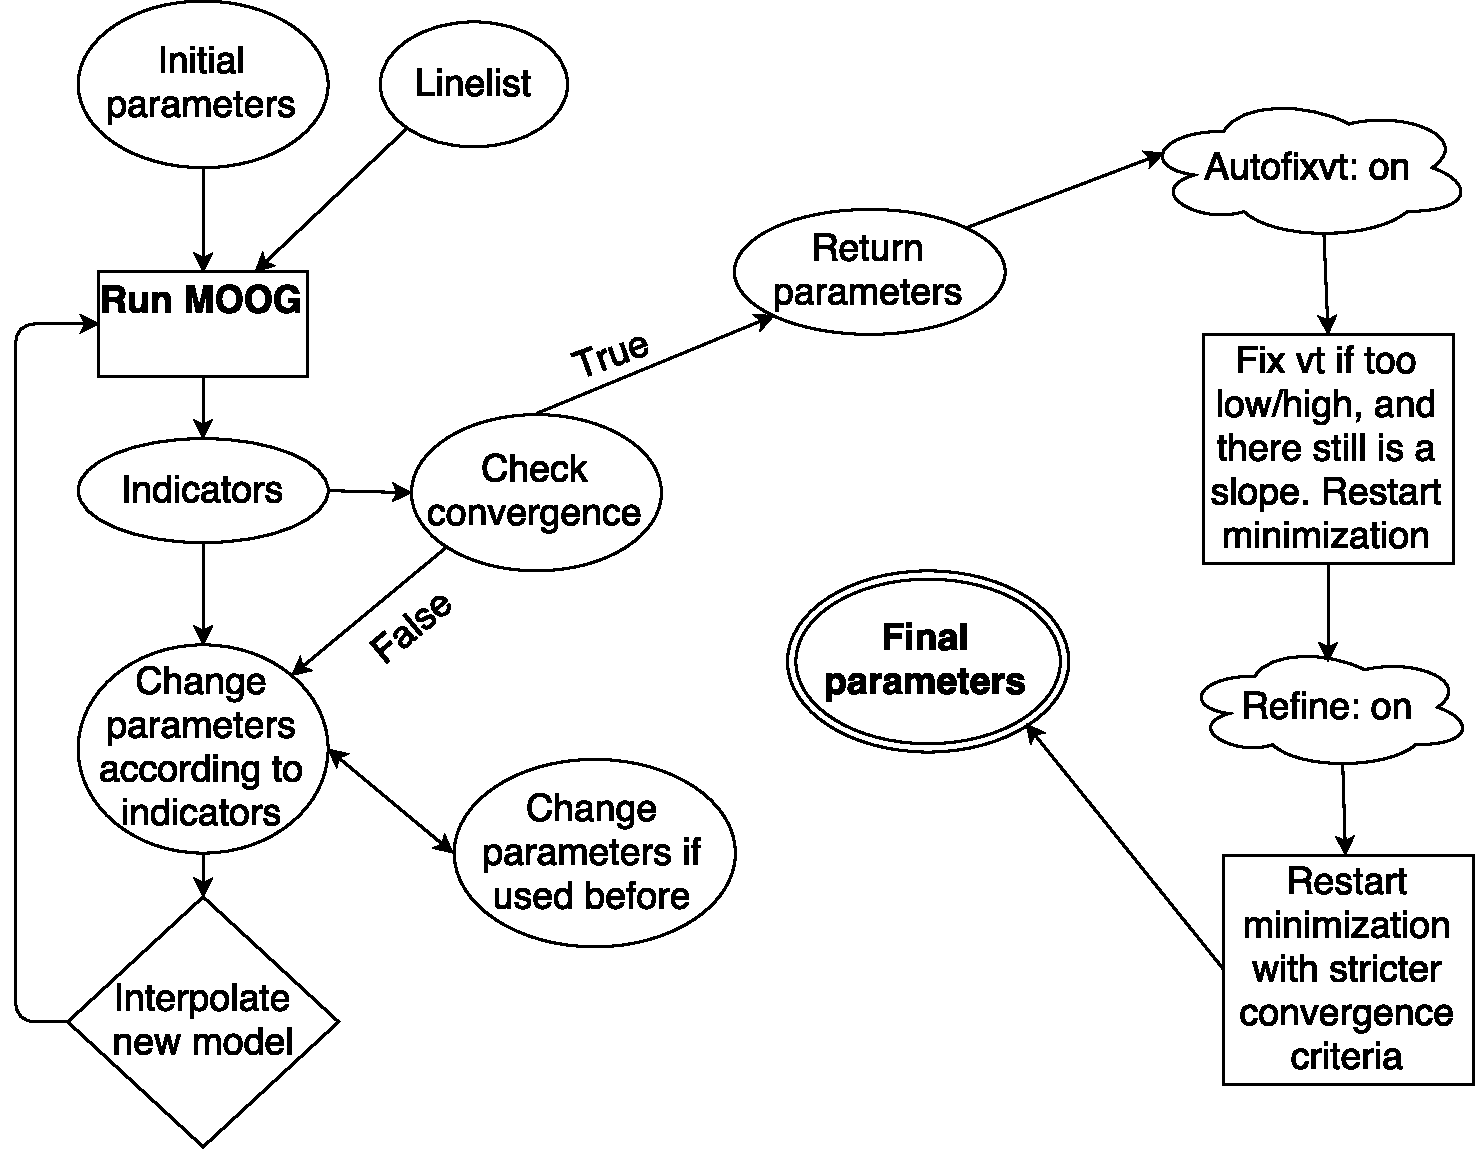
\includegraphics[width=1.0\linewidth]{figures/FASMA_minimization.pdf}
    \caption{Overview of the minimization for \FASMA. Credit: \citet{Andreasen2017a}.}
    \label{fig:minimization}
\end{figure}

\subsection{Error estimate}

%!TEX root = thesis.tex
\chapter{Results for FGK stars}
\label{cha:results}
\epigraph{Don't cry because it's over, smile because it happened.}{Dr. Seuss}

It is time to apply the theory and methodology on some data. In this chapter results from studies
during the thesis will be presented. There is the analysis of three stars which lead to two papers,
HD20010 \citep{Andreasen2016} and Arcturus \& 10 Leo \citep{Andreasen2017b}. A small summary of the
stars and their characteristics can be found in \tref{tab:stars}. More details will be provided in
the individual sections below for each star. Additionally, there was an analysis of how a cut in
excitation potential might affect the final parameters of a star. This will be discussed in
\sref{sec:EPcut}, and last the analysis of a range of synthetic spectra from the PHOENIX spectral
library \citep{Husser2013}, with $T_\mathrm{eff}$ lower than analysed in previous stars with the
methodology described above in \sref{sec:parameters}. However, before diving into the results of the
analysis it is important to describe how the NIR line list were compiled and why and how it was
later refined.

\begin{table*}[htb!]
    \caption{Summary of the four stars used in this thesis. The stellar parameters
             are from the PASTEL catalogue \citep{Soubiran2016} (see text for
             details), except the parameters for the Sun.}
    \label{tab:stars}
    \centering
    \begin{tabular}{lllllll}
      \hline\hline
        Star        & Spectrographs  & Resolution  & $T_\mathrm{eff}$ (K) &  $\log g$ (dex)  &   $\xi_\mathrm{micro}$ (km/s)   & [Fe/H] (dex)      \\
      \hline
        Sun         & FTS            & 600\,000    & $5777$               &  $4.44$          &    $1.00$                       & $ 0.00$          \\
        Arcturus    & FTS            & 100\,000    & $4300 \pm 111$       &  $1.60 \pm 0.29$ &    $1.93 \pm 0.17$              & $-0.54 \pm 0.11$ \\
        HD 20010    & CRIRES         & 100\,000    & $6152 \pm  95$       &  $3.96 \pm 0.11$ &    $1.17 \pm 0.24$              & $-0.27 \pm 0.06$ \\
        10 Leo      & CRIRES         & 100\,000    & $4742 \pm  61$       &  $2.76 \pm 0.17$ &    $1.45 \pm 0.08$              & $-0.03 \pm 0.02$ \\
      \hline
    \end{tabular}
\end{table*}

\section{The creation of a NIR line list}
\label{sec:creation_line_list}

As discussed extensively in \cref{cha:theory} and \cref{cha:method}, an atomic line list is needed
for employing the method described here. This line list is made by neutral and ionized iron lines in
the NIR. This has already been mentioned in \cref{cha:theory}. Here the process will be explained in
greater detail below for the two versions presented in \citet{Andreasen2016} and
\citet{Andreasen2017a}, respectively.


\subsection{First version}
\label{sec:linelist_first}

The first version of a NIR iron line list for determining stellar atmospheric parameters of high
resolution and high S/N spectra were presented in \citet{Andreasen2016}. Other NIR line lists exists
such as the one from \citet{Onehag2012,Lindgren2016} for utilising the synthetic method described
above\unfinished{Add more line lists from the literature.}. Here all iron transitions between
\SIrange{10000}{25000}{\angstrom}\footnote{That is equivalent to the YJHK bands.} were downloaded
from the VALD database \citep{VALD1,VALD2}. This only includes \ion{Fe}{I} and \ion{Fe}{II}
transitions. In total were \num{50198} \ion{Fe}{I} and \num{28339} \ion{Fe}{II} lines respectively
acquired.

The EW of all lines were measured in the solar atlas by \citet{Hinkle1995}. The EWs were measured
using \ARES due to the large amount of lines and to be as consistent as possible in the
measurements. Since \ARES expect a 1D spectrum with equidistant wavelength step, the solar spectrum
was interpolated onto a regular wavelength grid of \SI{0.01}{\angstrom}. This did not change the
appearance, and hence not the EW, of the final spectrum. This wavelength step is equivalent to a
spectral resolution of \num{1500000} at \SI{15000}{\angstrom}.

The EWs were measured by fitting Gaussian profiles to the spectral lines. For a given line, \ARES
output the central wavelength of the line (provided in the line list), the FWHM maximum of the
fitted line, the number of lines fitted for the final result (in case of blending), the depth of the
line, the EW of the line, and the Gaussian coefficients of the line. In the latest version of \ARES,
the error of the EW is also provided \citep{Sousa2015a}.

More lines were discarded according to the following four criteria:

\begin{itemize}
  \item Lines with EW lower than \SI{5}{m\angstrom} as these lines can be problematic to see in
        spectra with lower S/N or spectra with many spectral features. Therefore the measurements
        of these lines are less reliable than stronger lines.
  \item Lines with EW higher than \SI{200}{m\angstrom} as these lines are too strong to be fitted
        with a Gaussian profile. These lines might also be saturated and do not contain information
        about the abundance (see \fref{fig:cog}).
  \item Lines where the total number of fitted lines are 10 or higher since they show indications of
        severe blending.
  \item If the fitted central wavelength is more than \SI{0.05}{\angstrom} away from the wavelength
        provided by VALD3 to avoid false identification. This should also remove some blended lines.
\end{itemize}
After this removal the number of \ion{Fe}{I} and \ion{Fe}{II} lines are reduced to \num{6060} and
\num{2735}, respectively.


\subsubsection{Visual removal of lines}

At this point a visual inspection were necessary. All absorption lines from all elements were
downloaded from the VALD3 database in a \SI{3}{\angstrom} window around each of the nearly
\num{9000} iron lines from the previous step. For each small spectral window, all absorption lines
(including the iron line(s)) were plotted on top of the solar spectrum. An iron line were discarded
if another line had the same central wavelength and/or the absorption line were severely blended.
Most of the discarded iron lines had high EP, which are weak compared to the low EP lines.
Therefore, it is fair to assume that many of these iron lines were falsely identified as another
stronger line from another element. After the visual removal the number of \ion{Fe}{I} and
\ion{Fe}{II} lines were reduced to a mere 593 and 22, respectively.

For some of the absorption lines it was not clear which element was the cause. These lines were
marked for further investigation with synthesis as described below.

\subsubsection{Synthetic investigation}

For the lines marked above for further investigation an even broader window were used of
\SI{6}{\angstrom}. Once again, all lines were downloaded from the VALD3 database in these spectral
windows. \MOOG were used with the \emph{synth} driver to create a synthetic spectrum using a solar
atmosphere model with $T_\mathrm{eff}=\SI{5777}{K}$, $\log g=4.438$, $A(\mathrm{Fe})=7.47$, and
$\xi_\mathrm{micro}=\SI{1.00}{km/s}$. The iron abundance (7.47) is from \citet{Gonzalez2000}. The
overall metallicity for the solar atmosphere model is $[\ion{M}/\ion{H}]=0.00$ by definition. This
was done for all spectral windows for three different $[\ion{Fe}/\ion{H}]=\{-0.2, 0.0, 0.2\}$.
Before creating a synthetic spectrum all elements which are more than singly ionised were removed
since \MOOG does not allow these. An example of this can be seen in
\fref{fig:synthetic_investigation}. Here the neutral iron line at \SI{15550.439}{\angstrom} were
investigated. The three coloured curves are synthetic spectra with the three different
$[\ion{Fe}/\ion{H}]$. Note that while $[\ion{Fe}/\ion{H}]$ is used as a proxy for the over
metallicity, $[\ion{M}/\ion{H}]$, it is here specific only the iron abundance that is changed. The
upper plot shows the result with the full VALD3 line list, while in the lower plot the iron line
were removed from the line list. In this case it is clear that the iron line is the cause of the
absorption line. The grey curve is the solar atlas for reference.

\begin{figure}[htpb!]
    \centering
    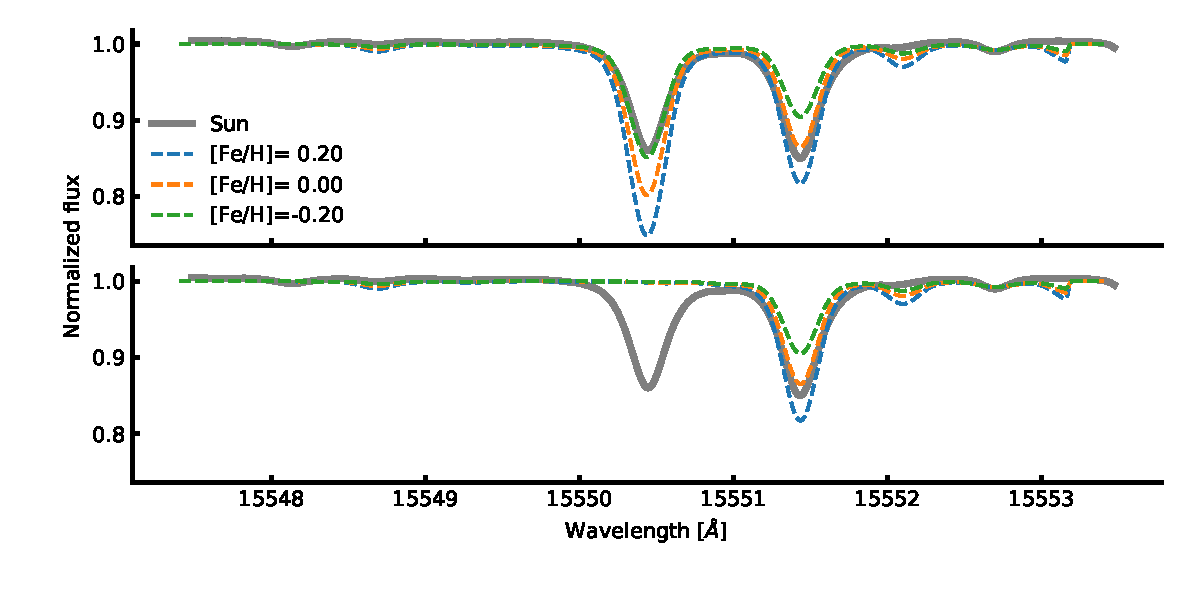
\includegraphics[width=1.0\linewidth]{figures/synthetic_investigation.pdf}
    \caption{The three coloured curves represents different iron abundance, $\{-0.2, 0.0, 0.2\}$ dex
             compared to solar abundance. The grey curve is the solar atlas for reference. In this
             case the iron line at \SI{15550.439}{\angstrom} is investigated. \emph{Upper} plot:
             Synthetic spectra were computed using the full VALD line list in the spectral range for
             the three different iron abundances. \emph{Lower} plot: Same as the upper plot, but
             with the iron line removed from the line list. Since the synthetic spectra shows no
             features at this absorption line anymore, it is a fair assumption to say the iron line
             is the cause of this absorption line.}
    \label{fig:synthetic_investigation}
\end{figure}

If the three synthetic spectra shows variation at the iron line of interest, then it is assumed that
the iron line is the cause for the absorption line. As a simple test, the iron line was also removed
from the line list used to create the synthetic spectra. If the iron line in the synthetic spectra
disappeared, it was a clear signal that this line can be used in the final iron line list ( this can
be seen clearly in the lower plot of \fref{fig:synthetic_investigation}). In some cases two iron
lines had the same or very similar wavelength, and this technique was used to include the right iron
line. In cases where both iron lines causes the absorption line, they were both discarded since they
are blended.

In a few cases two iron lines had the same wavelength and EP but different $\log \mathit{gf}$. If
these both cause an iron line they can be combined into a single line by adding their $\mathit{gf}$
values. After this step, there was 414 \ion{Fe}{I} lines and 12 \ion{Fe}{II} lines, respectively.



\subsubsection{Calibrating the line list: astrophysical $\log \mathit{gf}$ values}

These lines were collected into a single line list in the format required by MOOG \citep{Sneden1973}
and the line abundance were measured by all lines using the solar atmosphere model described above.
If the derived abundance for a single line differs by more than 1.0 dex from the solar iron
abundance, the line would be discarded. The solar iron abundance used is 7.47 as found by
\citet{Gonzalez2000}. \unfinished{Why do we remove above 1.0dex?}

After the removal of the lines mentioned above, the final line list is almost compiled. At this
point the line list has to be calibrated. This is done by changing $\log \mathit{gf}$ so the line
abundance for all iron lines are 7.47 when using the solar atmosphere model mentioned above. As
mentioned in \sref{sec:linelist} there is a anti-correlation between the abundance of a line and
$\log \mathit{gf}$. This means a bisector minimization can be used to locate the $\log \mathit{gf}$
that gives the desired abundance.

This was done for all the iron lines at this stage. It is important to calibrate a line list if the
setup of parameter determination is changed somehow. This includes the type of model atmospheres
used (e.g. ATLAS9 or MARCS), the interpolation code to generate a model atmosphere from the grid, or
the settings of the radiative code, here \MOOG.


\subsubsection{Removal of high dispersion lines}

The line list calibrated above was used to derive parameters for HD 20010 (see \sref{sec:HD20010}),
however the derived parameters showed poor results when compared to the literature values. This lead
to the following test, where highly disperse lines would be removed.

A Gaussian distribution was made for the EW of each line centred on the EW itself,
\begin{align}
  f(x, EW, \sigma) = \frac{1}{\sqrt{2\pi\sigma^2}} e^{-\frac{(x-EW)^2}{2\sigma^2}},
\end{align}
where $\sigma$ is the error on the EW, expressed by \citet{Caryel1988}:
\begin{align}
  \sigma \simeq 1.6 \frac{\sqrt{\Delta\lambda EW}}{S/N},
\end{align}
where $\Delta\lambda=0.1$ and a S/N=50 is considered here, which is much lower than the actual S/N
of the solar atlas. 100 draws of the distribution above were made for each line and derive the
abundance using the solar atmosphere model. The mean absolute deviation (MAD) were calculated for
each line abundance. The MAD for each line as a function of the original measured EW can be seen in
\fref{fig:dispersive_lines}. The trend for the weaker lines is expected since a small absolute
change in the EW results in a large relative change in abundance. However, this does not mean these
lines have a high dispersion. Therefore the disperse lines are found in the de-trended MAD value,
where an exponential function is used for de-trending. A single point above $3\sigma$ is removed
iteratively in the de-trended data. After this process there are 334 \ion{Fe}{I} lines and 13
\ion{Fe}{II} lines.

\begin{figure}[htpb!]
    \centering
    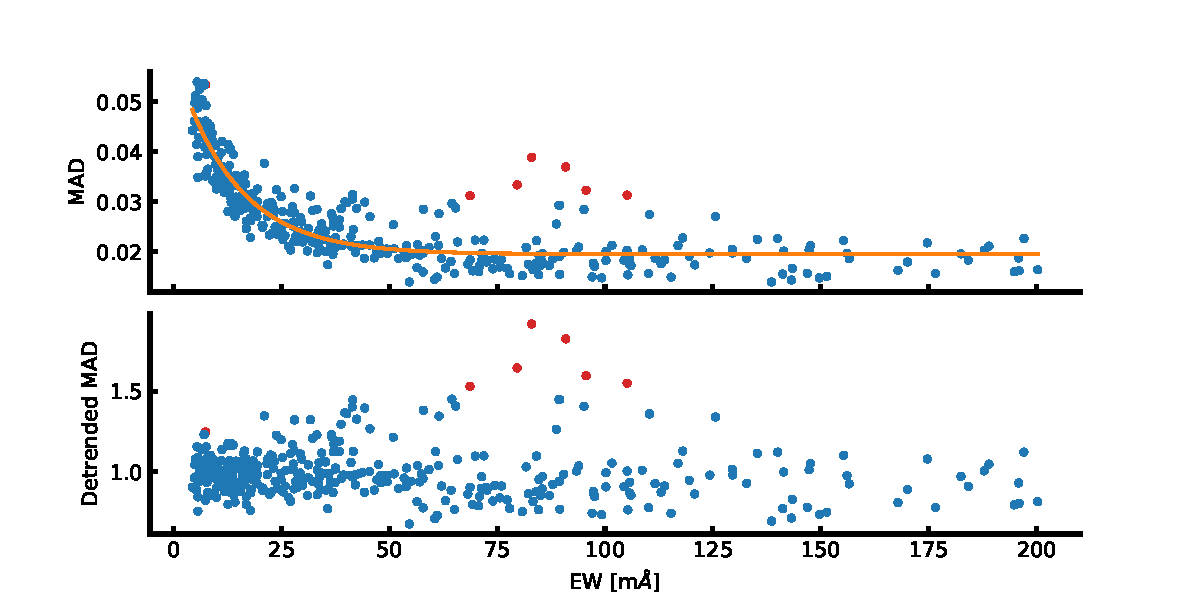
\includegraphics[width=1.0\linewidth]{figures/disperse_lines.pdf}
    \caption{The most disperse lines. \emph{Upper} plot: The MAD versus the original EW. The red
             points are the outliers which were discarded during this process. \emph{Lower} plot:
             Same as above with the MAD being de-trended by the exponential fit as shown in the
             upper panel.}
    \label{fig:dispersive_lines}
\end{figure}



\subsection{Second version}
\label{sec:linelist_second}

As will be seen in \sref{sec:HD20010_first} the line list presented above were used to derive
atmospheric parameters of HD 20010. Even though the first test of the line list was success-full,
it left room for improvements. The errors on the derived parameters were quite high for the spectral
type compared results obtainable with a similar analysis utilising the optical spectrum (see
\sref{sec:HD20010_first} for details on this\unfinished{Make sure to actually discuss this!}).
Additionally, the derived metallicity was 0.10 dex higher than the literature values used.

If all derived parameters except metallicity are reliable (when compared to e.g. a literature
value), then it suggest that the measured EW are either over- or underestimated. However, when using
a line list for the first time like here, it can also suggest problems with the line list itself,
for example a bad calibration. This could have been wrong measurements of the EWs of the calibrator
star, Sun in this case. This combines to several cases:
\begin{itemize}
  \item Correct measurement of EW of calibrator star:
  \begin{itemize}
    \item Systematic lower measurement of EW of target star leads to underestimated $[\ion{M}/\ion{H}]$
    \item Systematic higher measurement of EW of target star leads to overestimated $[\ion{M}/\ion{H}]$
    \item Correct measurement of EW of target star leads to correct $[\ion{M}/\ion{H}]$
  \end{itemize}
  \item Systematic lower measurements of EW of calibrator star:
  \begin{itemize}
    \item Systematic lower measurement of EW of target star leads to underestimated $[\ion{M}/\ion{H}]$
    \item Systematic higher measurement of EW of target star can lead to correct or overestimated $[\ion{M}/\ion{H}]$
    \item Correct measurement of EW of target star leads to underestimated $[\ion{M}/\ion{H}]$
  \end{itemize}
  \item Systematic higher measurements of EW of calibrator star:
  \begin{itemize}
    \item Systematic lower measurement of EW of target star can lead to correct or underestimated $[\ion{M}/\ion{H}]$
    \item Systematic higher measurement of EW of target star leads to overestimated $[\ion{M}/\ion{H}]$
    \item Correct measurement of EW of target star leads to overestimated $[\ion{M}/\ion{H}]$
  \end{itemize}
\end{itemize}
It is important to note, that \emph{correct} has been used here, assuming a perfect setup, that
includes perfect model atmosphere, perfect radiative transfer code, etc. In reality the final
$[\ion{M}/\ion{H}]$ (and the other parameters) measured by different group will occasionally differ
regarding the setup used.

As described in \sref{sec:linelist_first} the EW of the Sun (calibrator star) was measured with
\ARES. A crucial option to set when using \ARES is the \code{rejt} parameter as mentioned in
\sref{sec:measureEW}. This option is used to place the continuum and will this directly affect the
measured EW. At the time of compiling the first version of the line list it seems the \code{rejt}
value used did not reflect the high S/N of the spectrum, thus placing the continuum too low and
thereby underestimate the EW.

In this second version of the line list, the goal is to:
\begin{enumerate}
  \item Make sure the EW measurements are as correct as possible by measuring them by hand
  \item Free of blended lines in cooler stars (K stars in this case)
\end{enumerate}
The second point is a similar exercise which was done in the optical by \citet{Tsantaki2013}, where
blended lines were removed from the larger line list by \citet{Sousa2008a}. This allowed to
determine the atmospheric parameters of stars colder than \SI{5000}{K}. However, the optical
spectrum still suffer for severely blended lines at low $T_\mathrm{eff}$, thus this method does not
work for M stars.

Both of the above steps were done at the same time, by measuring the EWs by hand using \code{IRAF}.
Whenever a line was difficult to reliably measure, i.e. a consistent measurement was not
possible/easy, it was discarded since it was blended. This can be seen in
\fref{fig:linelist_comparison} where the EW measurements from the first version is shown against
this version with the manual measurements. There are some measurements of EW higher than
\SI{150}{m\angstrom} which should have been removed. These lines have not been used during the
analysis, however they were kept since they might appear useful on a later stage.

\begin{figure}[htpb!]
    \centering
    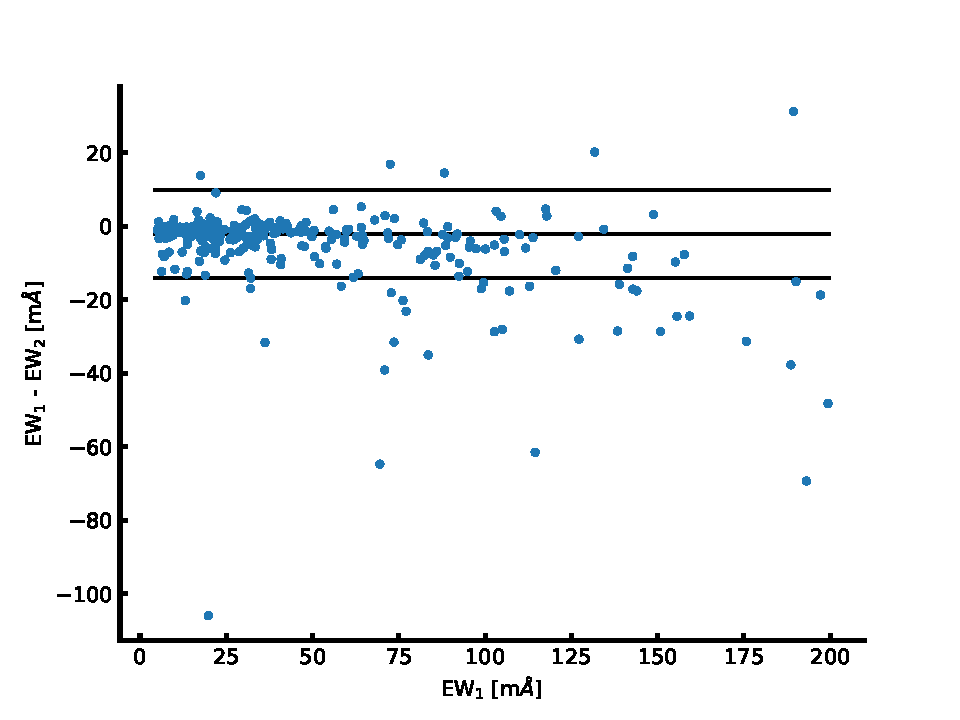
\includegraphics[width=1.0\linewidth]{figures/linelist_comparison.pdf}
    \caption{Comparison of the EW from the first version of the line list, EW$_1$, and the second
             version, EW$_2$. The EWs are generally higher in the second version, with an average
             difference between the two version of \SI{2.1+-11.1}{m\angstrom}. The three horizontal
             lines show the average value and the standard deviation.}
    \label{fig:linelist_comparison}
\end{figure}

While the first version might seem careless since it is necessary with a second version, it is
important to stress the 1) limited access on high quality of NIR spectra, and 2) the gained
experience during the course of the thesis which proved valuable in the refining of the line list
by a second visual inspection of the line list on the solar spectrum.

After the new measurements of the EWs, the line list was re-calibrated according to the procedure
described above. The change in $\log \mathit{gf}$ is \SI{-0.062+-0.157}, i.e. on average the
oscillator strengths are higher in the second version compared to the first version of the line
list.

With the second version there are only 5 \ion{Fe}{II} lines which is a concern since these are
crucial for the derivation of the surface gravity. Therefore, when possible, it is important to
obtain the $\log g$ from other more reliable studies.


\section{HD20010}
\label{sec:HD20010}

HD 20010 is a star that has been analysed twice with the methodology described here in this thesis.
First time this star was analysed was in \citet{Andreasen2016} when the NIR line list was published
(see \sref{sec:linelist_first}). Later this line list was revised leading to a removal of several
lines (see \sref{sec:linelist_second}). This resulted in the second analysis in
\citet{Andreasen2017b}; both described below.

\subsection{First analysis}
\label{sec:HD20010_first}

To test the first version of the NIR line list a well-studied solar-type star is needed. The
spectrum for such a target needs to be available in the NIR at both high resolution and high S/N. An
ideal place to look for such a star is the CRIRES-POP database \citep{Lebzelter2012}. Here, the best
target for testing is HD 20010, an F8 subgiant star. At the time of writing this thesis and
\citet{Andreasen2016} the spectrum of HD 20010 was not fully reduced. Here it is still contaminated
by some telluric lines, and the wavelength solution used is not optimal. Both things are essential,
however a tedious and difficult task to accomplish.

HD 20010 star has been part of many surveys and is therefore well studied. Different parameters from
the literature are listed in \tref{tab:HD20010}.

\begin{table*}[htb!]
    \caption{Selection of literature values for the atmospheric parameters for HD20010. The mean and
             a $3 \sigma$ standard deviation is presented at the end of the table from the
             literature values included, which we use as a reference for our derived parameters.}
    \label{tab:HD20010}
    \centering
    \begin{tabular}{l|llll}
      \hline\hline
     Author                 & $T_\mathrm{eff}$ (K) & $\log g$ (dex)  & $[\ion{Fe}/\ion{H}]$ (dex)  & $\xi_\mathrm{micro}$ (km/s)  \\
      \hline
    \cite{Balachandran1990} & $6152$               & $4.15$          & $-0.27 \pm0.08$             & $1.60$                       \\
    \cite{Favata1997}       & $6000$               & \ldots          & $-0.35 \pm0.07$             & \ldots                       \\
    \cite{Santos2004}       & $6275\pm57$          & $4.40\pm0.37$   & $-0.19 \pm0.06$             & $2.41\pm0.41$                \\
    \cite{Gonzalez2010}     & $6170\pm35$          & $3.93\pm0.02$   & $-0.206\pm0.025$            & $1.70\pm0.09$                \\
    \cite{Ramirez2012}      & $6073\pm78$          & $3.91\pm0.03$   & $-0.30 \pm0.05$             & \ldots                       \\
    \cite{Mortier2013}      & $6114$               & \ldots          & $-0.19$                     & \ldots                       \\
      \hline
      Mean                  & $6131\pm255$         & $4.01\pm0.60$   & $-0.23 \pm0.14$             & $1.90\pm1.08$                \\
      \hline
    \end{tabular}
\end{table*}

The data available at CRIRES-POP are in the raw format and pipeline reduced, while three small
pieces of the spectra are fully reduced on the web
page\footnote{\url{http://www.univie.ac.at/crirespop/data.htm}}. The data is in the standard CRIRES
format with each fits file including four binary tables with the data from the four detectors. In
the future, the final reduced data will be presented by the CRIRES-POP team. In contrast to the
pipeline reduced data, this will be of higher quality, a better wavelength calibration, and telluric
correction. The EWs were measured of the pipeline reduced spectra, and where there was an overlap
with the fully reduced spectrum, we measured both as a consistency check. The measured EWs from the
fully reduced spectra were consistent with the measured EWs from the pipeline reduced spectra. As
mentioned above, the Y, J, H, and K-bands, which are all available for this star, were used in this
analysis. The spectra come in pieces of \SIrange{50}{120}{\angstrom}. These pieces overlap each
other, and up to five EW measurements were made for some lines. Unfortunately, wavelength
calibration is a difficult task for CRIRES owing to the rather small spectral regions measured on
each detector. Each calibration was performed separately for each detector and required the
availability of a sufficient number of calibration lines in the respective spectral region. This was
not always the case and a default linear solution was applied. A pipeline reduced spectrum shows up
as a stretched spectrum if the wavelength calibration is poor compared to a model spectrum or a
solar spectrum, for example. The wavelength calibration does not have any effect on the
signal-to-noise ratio, which is generally high for the spectrum of HD 20010. The signal-to-noise
varies between 200 and 400 for different chunks. However, the stretched spectra will most likely
have an effect on the measured EWs. The pipeline reduced spectra for HD 20010 contains tellurics and
the wavelength is shifted in radial velocity. All of these factors make the line identification very
difficult, so a program was developed\footnote{The program (and other small scripts) can be found
here\url{https://github.com/DanielAndreasen/astro_scripts}} to properly identify the lines, which
does the following:

\begin{enumerate}
  \item Plotting the observed spectrum
  \item Overplotting a model spectrum. In this particular case the solar spectrum was used since the
        atmospheric parameters are close enough, so the sun was able to serve as a model
  \item Overplotting a telluric spectrum from the TAPAS web page \citep{Bertaux2014}
  \item Overplotting vertical lines at the location of lines in the list
  \item Calculating the cross-correlation function (CCF) for the telluric spectrum with respect to
        the observed spectrum, locating the maximum value by a Gaussian fit, and using this to shift
        the telluric spectrum with the found RV
  \item Performing the same as step 5, but for the model spectrum
  \item Shifting the lines with the same RV as found for the model/solar spectrum
\end{enumerate}

The final plot shows the shifted spectra, and the CCFs at the sides. An example of the software in
use is shown in \unfinished{Make a plot of this}. The two radial velocities (for the telluric and
model spectrum) are part of the title of the plot. Once the lines were identified, the EWs were
measured with the \code{splot} routine in \emph{Image Reduction and Analysis Facility}
(\code{IRAF}). The reason not to choose \ARES for this task was to visually confirm the
identification of the line given the relative poor wavelength calibration from the automatic
pipeline. We were able to measure 249 \ion{Fe}{I} lines and 5 \ion{Fe}{II} lines compared to 344
\ion{Fe}{I} lines and 13 \ion{Fe}{II} lines for the Sun over the whole NIR spectral region in the
first version of the line list. Whenever there were more than one EW measurement of a line, the
average was used for the final EW. The stellar atmospheric parameters were derived using the
standard procedure (see \sref{sec:parameters}). Lines below \SI{5}{m\angstrom} were removed in order
to remove the lines which are most affected by contamination from either telluric or other line
blends. Additionally, a cut in EP at \SI{5.5}{eV} was made since the \ion{Fe}{I} and \ion{Fe}{II}
lines usually used for stellar parameter determination in the optical regime are also limited to
similar values \citep[see e.g][]{Sousa2008a}. Higher excitation potential lines are also more likely
to be affected by non-LTE effects.

The parameters were derived with one outlier in abundance removed iteratively (after a completed
minimization) until no outliers were present. Since we could only measure 5 \ion{Fe}{II} lines, the
parameter were also derived with $\log g=4.01$ dex fixed at the reference mean value (see
\tref{tab:HD20010}). The resulting atmospheric parameters and iron abundances are presented in
\tref{tab:HD20010_results}. The effective temperature, surface gravity, and metallicity agree within
the errors with the literature values. Similar parameters are obtained by fixing $\log g$ to the
average literature value or by leaving it free.

\begin{table*}[htb!]
    \caption{The derived parameters for HD20010 with and without fixed surface gravity.}
    \label{tab:HD20010_results}
    \centering
    \begin{tabular}{lllll}
      \hline\hline
                     & $T_\mathrm{eff}$ (K) &  $\log g$ (dex)  &   $\xi_\mathrm{micro}$ (km/s)  & [Fe/H] (dex)      \\
      \hline
        Literature   & $6131 \pm 255$       &  $4.01 \pm 0.60$ &    $1.90 \pm 1.08$              & $-0.23 \pm 0.14$ \\
      \hline
                     & $6116 \pm 224$       &  $4.21 \pm 0.58$ &    $2.45 \pm 0.45$              & $-0.14 \pm 0.14$ \\
                     & $6144 \pm 212$       &   4.01 (fixed)   &    $2.66 \pm 0.42$              & $-0.13 \pm 0.29$ \\
      \hline
    \end{tabular}
\end{table*}


The errors on the atmospheric parameters for HD 20010 are much higher than what is achievable with
other measurements in the literature, as presented above in \tref{tab:HD20010}. In order to explain
these errors, we calculated the abundances for all lines which have at least two measurements of the
EW. We then calculated the abundances for the highest measured EW and the lowest. The differences in
abundances are presented in \fref{fig:HD20010abundance}. The very large differences (more than 0.1
dex) translate to the high errors in the parameters.

\begin{figure}[htpb!]
    \centering
    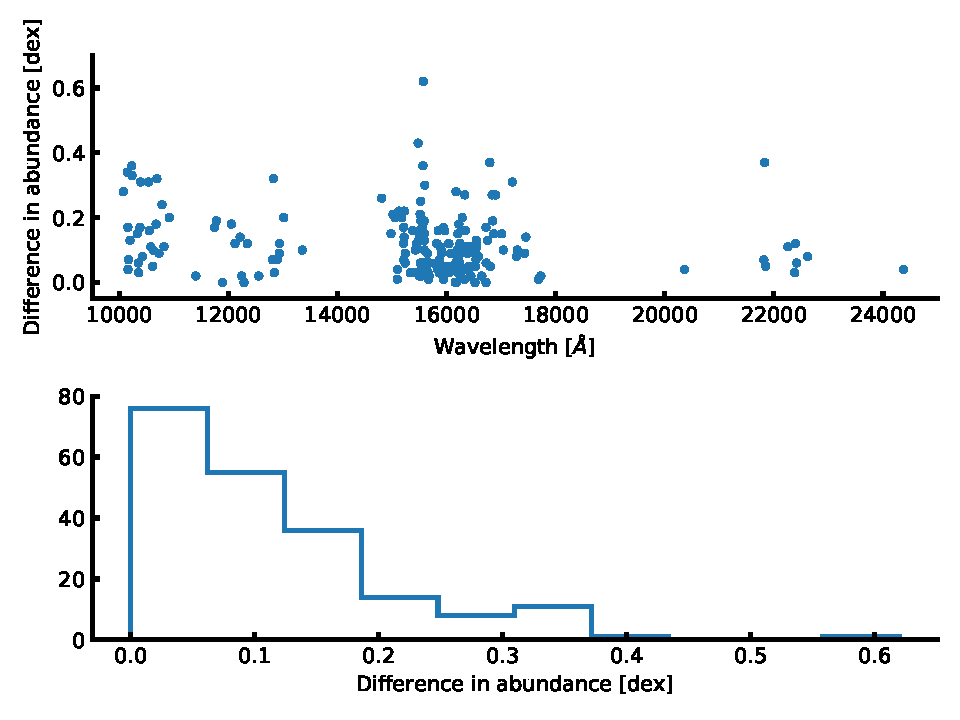
\includegraphics[width=0.8\linewidth]{figures/HD20010abundance_error.pdf}
    \caption{Difference in abundance for HD 20010 when multiple measurements of EW were obtained.
             The differences are between the lowest and highest measured EW in case of multiple
             measurements. This is shown against the wavelength (\emph{upper panel}) and in a
             histogram (\emph{lower panel}).}
    \label{fig:HD20010abundance}
\end{figure}


This test strongly suggest that errors in the EWs, likely due to the telluric contamination and
non-optimal reduction of the spectrum (poor default wavelength calibration), are responsible for the
relatively large error in the derived stellar parameters. After the first analysis of HD 20010, the
CRIRES-POP team published a fully reduced spectrum of 10 Leo \citep{Nicholls2017} with telluric
correction and an optimal wavelength solution. The results obtained from this star (see
\sref{sec:10Leo}) are very promising for the method used here, and it encourage a complete re-visit
of HD 20010 once the reduction is optimal.


\subsection{Second analysis}
\label{sec:HD20010_second}

During the analysis of Arcturus (see \sref{sec:arcturus}) and 10 Leo (see \sref{sec:10Leo}) with the
refined line list presented in \sref{sec:linelist_second} it was a simple task to apply the updated
line list on HD 20010 a second time as a test whether it would perform similar, worse or better.
This is compared to results obtained from the literature.

Therefore HD 20010 was revisited, and the atmospheric stellar parameters was derived. The measured
EWs from the results above in \sref{sec:HD20010_first} was kept, however the lines which did not
make the cut in the second version of the line list was removed. Moreover, the $\log \mathit{gf}$
values was updated since these were re-calibrated.

\FASMA was used to obtain the results which are shown in \tref{tab:results} along with the results
for Arcturus and 10 Leo (details on their parameters will be found below). The agreement with the
adopted average literature values are better for HD 20010 compared to the results from above in
\sref{sec:HD20010_first} (especially $[\ion{Fe}/\ion{H}]$ and $\log g$), and smaller errors with the
updated results. This first test of the line list already shows promising results. The literature
values are slightly different here than compared to the first analysis of this star. This is solely
because other references were used, the PASTEL catalogue \citep{Soubiran2016}. However, this does
not change the improvement seen.


\begin{table}[htb!]
    \caption{Results for the three stars where first set of parameters are the literature values as
             presented in \tref{tab:stars}, second set of parameters are results with $\log g$ set
             to the same value during the minimization procedure as found in the literature (fixed),
             and last set of parameters are with all parameters free during the minimization
             procedure.}
    \label{tab:results}
    \centering
    \begin{tabular}{llll}
      \hline\hline
                                    & HD 20010          &  10 Leo           &  Arcturus        \\
      \hline
        Literature                  &                   &                   &                  \\
        $T_\mathrm{eff}$ (lit.)     & $6152 \pm  95  $  &  $4741 \pm  60  $ & $4300 \pm 110  $ \\
        $\log g$ (lit.)             & $3.96 \pm 0.19 $  &  $2.76 \pm 0.17 $ & $1.60 \pm 0.29 $ \\
        $[\ion{Fe}/\ion{H}]$ (lit.) & $-0.27 \pm 0.06$  &  $-0.03 \pm 0.02$ & $-0.54 \pm 0.11$ \\
        $\xi_\mathrm{micro}$ (lit.) & $1.17 \pm 0.24 $  &  $1.45 \pm 0.08 $ & $1.93 \pm 0.13 $ \\
      \hline
        $\log g$ fixed              &                   &                   &                  \\
        $T_\mathrm{eff}$            & $6161 \pm 164  $  &  $4761 \pm 118  $ & $4357 \pm  74  $ \\
        $\log g$                    & 3.96 (fixed)      &  2.76 (fixed)     & 1.60 (fixed)     \\
        $[\ion{Fe}/\ion{H}]$        & $-0.18 \pm 0.11$  &  $ 0.01 \pm 0.07$ & $-0.55 \pm 0.04$ \\
        $\xi_\mathrm{micro}$        & $1.72 \pm 0.44 $  &  $1.25 \pm 0.11 $ & $1.55 \pm 0.10 $ \\
      \hline
        All free                    &                   &                   &                  \\
        $T_\mathrm{eff}$            & $6162 \pm 184  $  &  $4805 \pm  98  $ & $4439 \pm  62  $ \\
        $\log g$                    & $4.08 \pm 0.77 $  &  $2.42 \pm 0.61 $ & $1.20 \pm 0.20 $ \\
        $[\ion{Fe}/\ion{H}]$        & $-0.18 \pm 0.11$  &  $-0.01 \pm 0.07$ & $-0.58 \pm 0.06$ \\
        $\xi_\mathrm{micro}$        & $1.59 \pm 0.49 $  &  $1.23 \pm 0.10 $ & $1.55 \pm 0.10 $ \\
        \hline\hline
    \end{tabular}
\end{table}




\section{Arcturus}
\label{sec:arcturus}

Arcturus is one of the brightest stars on the night sky with a V magnitude of -0.05
\citep{Ducati2002}. Hence it is a prime target for testing with the numerous measurements of the
atmospheric parameters as mentioned above.

The atlas consists of both a summer observation set and a winter observation set. The two data sets
have been obtained in order to minimise the effect of tellurics at different spectral regions. A
comparison between the two sets of measured EWs - both the manual measurements using IRAF and the
% automatic measurements using \ARES - are shown in Fig.~\ref{fig:EWcomp}. The automatic EW
measurements for the summer set and winter set show excellent agreement with a dispersion of
\SI{7}{m\angstrom}. This means that the two data sets are very similar, thus we decided to only
manually measure the EWs for one set (summer). We did, however, measure a few lines from the winter
data set to verify the agreement. Since the EWs are very similar we chose to only derive parameters
of the summer set with EWs measured with \ARES. Parameters were derived with and without $\log g$
set to a fixed value (1.60\,dex, the average literature value adopted). The derivation of the
parameters followed the procedure presented in Paper I, although we used the minimization routine of
FASMA \citep{Andreasen2017a}. After we reached convergence using all the iron lines we were able to
measure, one outlier above $3\sigma$ in abundance were removed, and the minimization routine was
restarted. This process was done iteratively until there were no more outliers. The final results
are presented in Table \ref{tab:results} together with mean parameters from the literature.

We generally see good agreement between the derived parameters and the average values from the
literature adopted (see Table \ref{tab:results}). The only parameter being difficult to measure is
the surface gravity due to the low number of \ion{Fe}{II} lines in the NIR. It is very important to
derive the metallicity accurately, and we report consistent results overall.


\section{10 Leo}
\label{sec:10Leo}

The approach for determining the atmospheric stellar parameters for 10 Leo is identical to Arcturus.
We use \ARES on each band (YJ, H, and K-band) separately. For the small gaps in the spectrum, we
simply set the flux to 1, since the spectrum is already normalised. This will also prevent \ARES to
identify and measure any lines in these regions. The EWs from the three regions are combined to one
final line list used for the determination of the parameters. The final results can be seen in
Fig.~\ref{fig:parameters} and Table~\ref{tab:results}.

Generally the derived parameters are in excellent agreement with the literature values listed here.
For $T_\mathrm{eff}$ we were \SI{64}{K} off with $\log g$ set as a free parameter, well within the
errors. The only parameter that show a discrepancy compared to the literature value is
$\xi_\mathrm{micro}$ with a difference of \SI{0.22}{km/s}, which is at the limit of the errors
reported. We note that this parameter is not reported in the PASTEL database, and this was a derived
parameter from a empirical relation. We were able to derive good $\log g$ values, although with
larger errors compared to the results from the literature.


\section{Synthetic cool stars}
\label{sec:synthetic_spectra}



\section{SWEET-Cat and parameters for 50 planet hosts}
\label{sec:SWEET-Cat}




\section{Parameter dependence on EP cut}
\label{sec:EPcut}

It is common practise, as in this case, to make a cut in EP for a line list when deriving
parameters. This was suggested in \citet{Andreasen2016} \citep[later done in][]{Andreasen2017b} for
the NIR line list used here. This cut was made at \SI{5.5}{eV}, inspired by a similar cut in the
optical \citep{Sousa2008a}, including only lines below this limit. The lines with higher EP might
also be affected by non-LTE effects which is not treated in this methodology.

As the parameters are dependent on this cut in EP\unfinished{Make a figure that shows this}, it
seemed interesting to divide a line list in two with upper and lower EPs and analyse those
separately. Before going into that analysis it is important to note, that the parameters should not
depend on any cut in EP if the theory is right, the radiative transfer code is working properly, and
the atmospheric models are correct. Lines with different EP are likely to be formed in different
layers of the atmosphere as discussed in \sref{sec:stellar_atmosphere}, however this should not
effect the final derived abundance, which is the problem here.

%!TEX root = thesis.tex


\chapter{SWEET-Cat}
\label{sec:SWEET-Cat}

Part of the work during the thesis has been dedicated to regularly update
SWEET-Cat\footnote{\url{https://www.astro.up.pt/resources/sweet-cat/}}, a catalogue with all
discovered planet hosts, and the stellar parameters.

In this chapter a detailed description of SWEET-Cat will be presented. Moreover an analysis of 50
planet hosts was performed during the thesis with updated planetary parameters (mass and radius).


\section{What is SWEET-Cat?}

As mentioned above, SWEET-Cat is a catalogue of planet host stars. However, the strength of
SWEET-Cat is the homogeneously analysed stars utilising the method described in
\sref{sec:parameters} with \code{FASMA} or a similar tool before the creation of \code{FASMA}.

In the era with a large number of discovered exoplanets (more than 3500 confirmed exoplanet at the
moment of writing), the time for in-depth statistical studies has arrived. However, when conducting
these studies it is crucial to have consistent measurements of e.g. stellar atmospheric parameters.
This can be obtained by using a single analysis to obtain these parameters, as it is know that
different methods will lead to different results \citep[see e.g.][for a recent review]{Hinkel2016}.

To obtain stellar atmospheric parameters from one method is an on-going goal with SWEET-Cat, where
high quality spectra are obtained for stars hosting planets. These are used to determine the stellar
parameters in a homogeneous way. All stars in SWEET-Cat analysed with the method from our group are
marked with a flag showing whether it is analysed homogeneously or not. The columns provided in
SWEET-Cat are summarised in \tref{tab:sweetcat}. It is important to note that SWEET-Cat does not
include any planetary parameters.

\begin{table}[htb!]
    \caption{Columns in SWEET-Cat}
    \label{tab:sweetcat}
    \centering
    \begin{tabular}{lrl}
      \hline\hline
      Column                         & Unit      & Description \\
      \hline
      Name                           &           & Popular stellar name                                 \\
      HD number                      &           & HD number                                            \\
      RA                             & \si{deg}  & Right ascension                                      \\
      Dec                            & \si{deg}  & Declination                                          \\
      $\mathrm{Vmag}$                & \si{mag}  & V magnitude                                          \\
      $\sigma(\mathrm{Vmag})$        & \si{mag}  & Error on V magnitude                                 \\
      $\pi$                          & \si{mas}  & Parallax                                             \\
      $\sigma(\pi)$                  & \si{mas}  & Error on parallax                                    \\
      Source of $\pi$                &           & Source of parallax measurement                       \\
      $T_\mathrm{eff}$               & \si{K}    & Effective temperature                                \\
      $\sigma(T_\mathrm{eff})$       & \si{K}    & Error on effective temperature                       \\
      $\log g$                       & \si{dex}  & Surface gravity                                      \\
      $\sigma(\log g)$               & \si{dex}  & Error on surface gravity                             \\
      $\log g_{\mathrm{LC}}$         & \si{dex}  & Surface gravity corrected from light curves          \\
      $\sigma(\log g_{\mathrm{LC}})$ & \si{dex}  & Error on surface gravity corrected from light curves \\
      $\xi_\mathrm{micro}$           & \si{km/s} & Micro turbulence                                     \\
      $\sigma(\xi_\mathrm{micro})$   & \si{km/s} & Error on micro turbulence                            \\
      $[\ion{Fe}/\ion{H}]$           & \si{dex}  & Metallicity                                          \\
      $\sigma([\ion{Fe}/\ion{H}])$   & \si{dex}  & Error on metallicity                                 \\
      Mass                           & $M_\odot$ & Stellar mass                                         \\
      $\sigma(\mathrm{Mass})$        & $M_\odot$ & Error on stellar mass                                \\
      Reference                      &           & Reference for parameters                             \\
      Homogeneity flag               & 0/1       & 0 for not homogeneous analysis, 1 otherwise          \\
      Last updated                   & date      & Last updated                                         \\
      Comments                       &           & Any special remarks/comments (e.g. M star)           \\
      \hline
    \end{tabular}
\end{table}

SWEET-Cat is updated on a weekly basis if new planet hosts are discovered, and whenever planet hosts
have been analysed with the method from our group, as described in this thesis.


\section{Data for 50 planet hosts}

In this section the data for a large update to SWEET-Cat will be described. The majority of the data
comes as a result from proposals submitted for observational time, while some of the data was found
in the archive. In the next section the analysis of the 50 spectra will be presented along with the
results.


\subsection{Proposals for observation time}

\unfinished{Well, nothing here...}

\subsection{Data collected from proposals}

Data for 43 out of the 50 stars were collected by the SWEET-Cat team using the UVES/VLT
\citep{UVES}, FEROS/2.2m telescope in La Silla \citep{FEROS}, and FIES/NOT \citep{FIES}
spectrographs. The remaining spectra were found in various archives. This includes spectra from the
HARPS/3.6m telescope in La Silla \citep{HARPS} and ESPaDOnS/CFHT \citep{ESPADONS}. Some
characteristics of the spectrographs are presented in \tref{tab:instruments} with the mean S/N for
the spectra used. The S/N for each star can be seen in \tref{tab:SCresults} along with the
atmospheric parameters of the stars. The S/N is measured automatically by ARES, however note that
ARES smoothes the spectra before measuring the S/N, hence it is listed higher than the actual S/N.
These 50 stars are confirmed exoplanet hosts listed in SWEET-Cat, but they belonged to the list of
stars that have not previously been analysed by our team.


\begin{table}[htb!]
    \caption{Spectrographs used for this paper with their spectral resolution,
             wavelength coverage, and mean S/N from the spectra used.}
    \label{tab:instruments}
    \centering
    \begin{tabular}{llll}
      \hline\hline
      Spectrograph & Resolution    & Spectral range            &   Mean S/N  \\
      \hline
      HARPS        &  \num{115000} & \SIrange{378}{691}{nm}    &   642       \\
      UVES         &  \num{110000} & \SIrange{480}{1100}{nm}   &   212       \\
      ESPaDOnS     &   \num{81000} & \SIrange{370}{1050}{nm}   &   775       \\
      FIES         &   \num{67000} & \SIrange{370}{730}{nm}    &   763       \\
      FEROS        &   \num{48000} & \SIrange{350}{920}{nm}    &   208       \\
      \hline
    \end{tabular}
\end{table}


\subsection{Data collected from archive}

The spectra was obtained with the highest possible resolution for a given spectrograph, and in cases
with multiple observations, we include all the observations unless a spectrum is close to the
saturation limit for a given spectrograph. For multiple spectra, we combine them after first
correcting the radial velocity (RV) and using a sigma clipper to remove cosmic rays. The individual
spectra are then combined to a single spectrum for a given star to increase the S/N. This single
spectrum is used in the analysis described below. For most of the spectra in the archive included
here, several spectra were combined as described above, while for the observations dedicated to this
work, the spectrum would be a single spectrum, or in cases of faint stars, it would be observed a
few times to reach the desired S/N. This is mostly due to the difference in science cases behind the
observations; for example, the HARPS spectra were used for RV monitoring or follow-up of the
exoplanet(s), while the UVES spectra were used to characterise stellar parameters.
\unfinished{Check this part}

\section{Analysis of 50 planet hosts}
\label{sec:sweetcat_analysis}

The method of determining atmospheric parameters from the curve of growth analysis has been applied
several times in the optical \citep[see e.g.][]{Mortier2013b,Tsantaki2013,Sousa2011,Santos2013}.
When studying stars with planets and any correlations between stellar and planetary parameters it is
important to have a homogeneous characterisation of the stars. An effort to create such a sample was
initiated by \citet{Santos2013} with the SWEET-Cat database. The motivation to homogenise the
stellar hosts is mainly to compare the hosts and make statistical studies on one consistent scale.
When doing these statistical studies, the results might otherwise suffer from offsets between
different methods.

The skills acquired during the NIR studies as mentioned above were directly translated into deriving
parameters for a sample of 50 known planet host stars that were not previously analysed by our group
\citep{Andreasen2017a}. The spectra of these stars were required at UVES, FIES, HARPS, and ESPaDOnS
with the mean S/N higher than 200\unfinished{Write more about the data acquisition here}.

A Hertzsprung-Russell diagram of the sample can be seen in \fref{fig:sweetcat}. The sample covers a
large range of $T_\mathrm{eff}$, FGK, while there are both dwarf, sub-giant, and some giant stars.
The colours indicate the $\log g$. In order to determine the luminosity of each star the simple
relation
\begin{align*}
  L = 4\pi R^2 \sigma T^4_\mathrm{eff}
\end{align*}
is used, where $L$ is the luminosity, $R$ is the stellar radius, and $\sigma$ is the
Stefan-Boltzmann constant. In solar units this relation is simply:
\begin{align*}
  \frac{L}{L_\odot} = \left(\frac{R}{R_\odot}\right)^2 \left(\frac{T_\mathrm{eff}}{T_{\mathrm{eff},\odot}}\right)^4
\end{align*}
In order to determine the the stellar radius, the empirical relation from \citet{Torres2010} was
used.

\begin{figure}[htpb!]
    \centering
    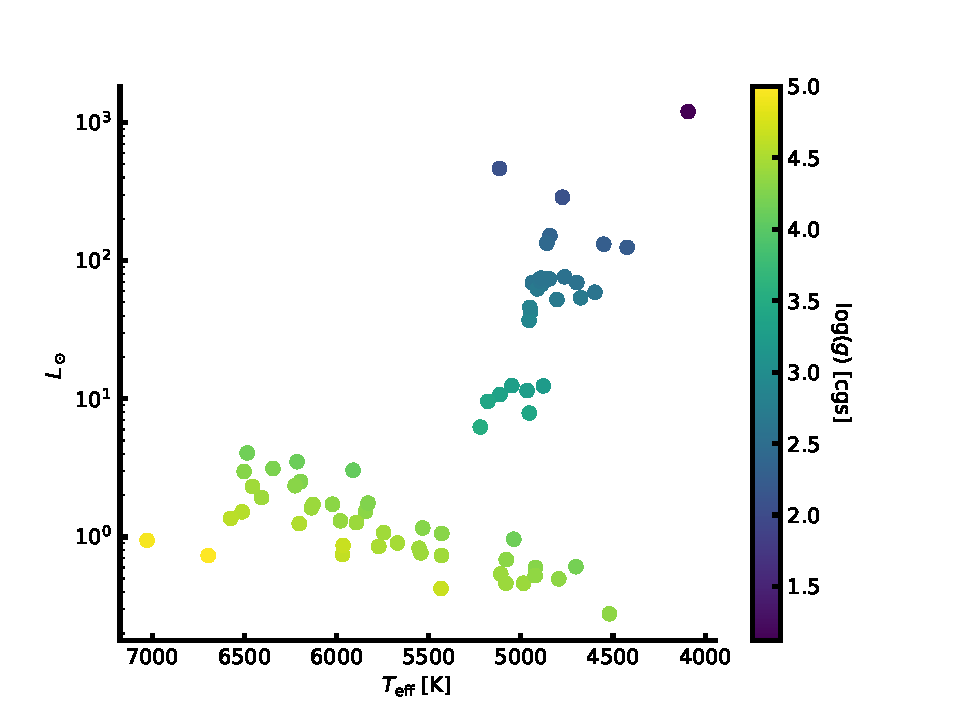
\includegraphics[width=1.0\linewidth]{figures/HR.pdf}
    \caption{A Hertzsprung-Russell diagram of the sample of 50 planet host stars added to SWEET-Cat.
             The parameters were derived using optical high resolution and high S/N spectra in
             tandem with \code{FASMA} and an optical line list. The colour scale shows the derived
             $\log g$ for each star.}
    \label{fig:sweetcat}
\end{figure}

The parameters were derived using \code{FASMA} with the optical line list compiled by
\citet{Sousa2008a} and \citet{Tsantaki2013} for stars where $T_\mathrm{eff}$ was below \SI{5200}{K}.
All the new derived parameters were added to SWEET-Cat, available for the community.

A correction to the spectroscopic surface gravity ($\log g_\mathrm{spec}$) is applied based on
asteroseismology as found by \citet{Mortier2014} given by:
\begin{align}
  \log g_\mathrm{seis} = \log g_\mathrm{spec} - (3.89\pm0.23)\times 10^{-4}\,T_\mathrm{eff}+2.10\pm0.14,
\end{align}
where $\log g_\mathrm{seis}$ is the corrected surface gravity. This correction is only used for FGK
dwarf stars, i.e. between $\SI{4800}{K}\leq T_\mathrm{eff}\leq\SI{6500}{K}$ and $\log
g\geq\SI{4.2}{dex}$. For stars with a $\log g$ lower than this limit the correction will not be
applied, and if the $\log g$ changes to below this limit after the correction, the spectroscopic
$\log g$ will be used again. The correction for $\log g$ depends on both $T_\mathrm{eff}$ and $\log
g$. The correction can be up to \SI{0.5}{dex}, depending on the $T_\mathrm{eff}$.

With these updated parameters the completeness of SWEET-Cat for stars brighter than V magnitude 10
is 85\% (77\% for stars brighter than 12). For fainter stars it is time expensive to acquire spectra
of the quality needed for this method. Moreover, many of the fainter planet host stars have been
observed with the \emph{Kepler} space mission, where most stars are faint.


\subsection{Habitable zone}
\label{sec:HZ}

The habitable zone of a star is at the distance where liquid water may exists. This distance depends
on $T_\mathrm{eff}$ and the luminosity, but also on the planetary atmosphere and its composition.
Using \citet[equation 3 described in][]{Kopparapu2013} to calculate the inner and upper limits of
the habitable zone. The equation is rather simple:
\begin{align}
 d = \sqrt{\frac{L/L_\odot}{S_\mathrm{eff}}} \si{AU},
 S_\mathrm{eff} = S_{\mathrm{eff},\odot} + aT_\ast + bT_\ast^2 + cT_\ast^3 + dT_\ast^4,
\end{align}
where $T_\ast=T_\mathrm-SI{5780}{K}$, and the coefficients can be found in Table 3 in
\citet{Kopparapu2013}, which depends on the specific model of habitable zone used. Here are used the
``Runaway Greenhouse'' for the inner limit and ``Maximum Greenhouse'' for the outer limit of the
habitable zone. The equation above is only valid for main sequence stars FGKM, thus only stars with
$\log g\geq\SI{4.2}{dex}$ have been included.


It was possible to find three planets within this zone; GJ 785 c, HD 37124 c, and KELT-6 c. These
planets does not have known radii, and their minimum masses are
$(0.076,\,0.652,\,3.710)M_\mathrm{Jupiter}$, respectively. Thus, it is fair to assume they are all
gas planets. All three host stars are metal-poor. A correlation between orbital period and host star
metallicity is known \citep[see e.g.][]{Adibekyan2013}, where metal-poor stars have planets with
higher orbital period. It is thus not a surprise that the three planets found in the habitable zone
all orbit a metal-poor star. A quick summary of the system is shown in \tref{tab:hz}.

\begin{table}[htb!]
    \caption{Host star and planetary properties of GJ 785, HD 37124, and KELT-6; all which have an
             exoplanet in the habitable zone.}
    \label{tab:hz}
    \centering
    \begin{tabular}{lrrr}
      \hline\hline
      Parameter            & GJ 785             & HD 37124           & KELT-6             \\
      \hline
      Stellar parameters   &                    &                    &                    \\
      \hline
      $T_\mathrm{eff}$     & \SI{5087(48)}{K}   & \SI{5460(35)}{K}   & \SI{6246(88)}{K}   \\
      $\log g$             & \SI{4.30(10)}{dex} & \SI{4.26(4)}{dex}  & \SI{4.22(9)}{dex}  \\
      $[\ion{Fe}/\ion{H}]$ & \SI{-0.01(3)}{dex} & \SI{-0.42(3)}{dex} & \SI{-0.22(6)}{dex} \\
      Luminosity           & $0.72L_\odot$      & $1.10L_\odot$      & $2.70L_\odot$      \\
      V magnitude          & 6.13               & 7.68               & 10.38              \\
      \hline
      Planetary parameters &                    &                    &                    \\
      \hline
      Planet               & GJ 785 c           & HD 37124 c         & KELT-6 c           \\
      Period               & \SI{525}{days}     & \SI{885}{days}     & \SI{1276}{days}    \\
      Mass                 & $0.076M_J$         & $0.652M_J$         & $3.710M_J$         \\
      Semi-major axis      & \SI{1.18}{AU}      & \SI{1.71}{AU}      & \SI{2.39}{AU}      \\
      Inner HZ limit       & \SI{0.86}{AU}      & \SI{1.04}{AU}      & \SI{1.56}{AU}      \\
      Outer HZ limit       & \SI{1.53}{AU}      & \SI{1.84}{AU}      & \SI{2.70}{AU}      \\
      \hline
    \end{tabular}
\end{table}

In \fref{fig:HZ} the habitable zone of the stars analysed here are shown along with the location of
the planets. The three systems mentioned above are highlighted in the figure.

\begin{figure}[htpb!]
    \centering
    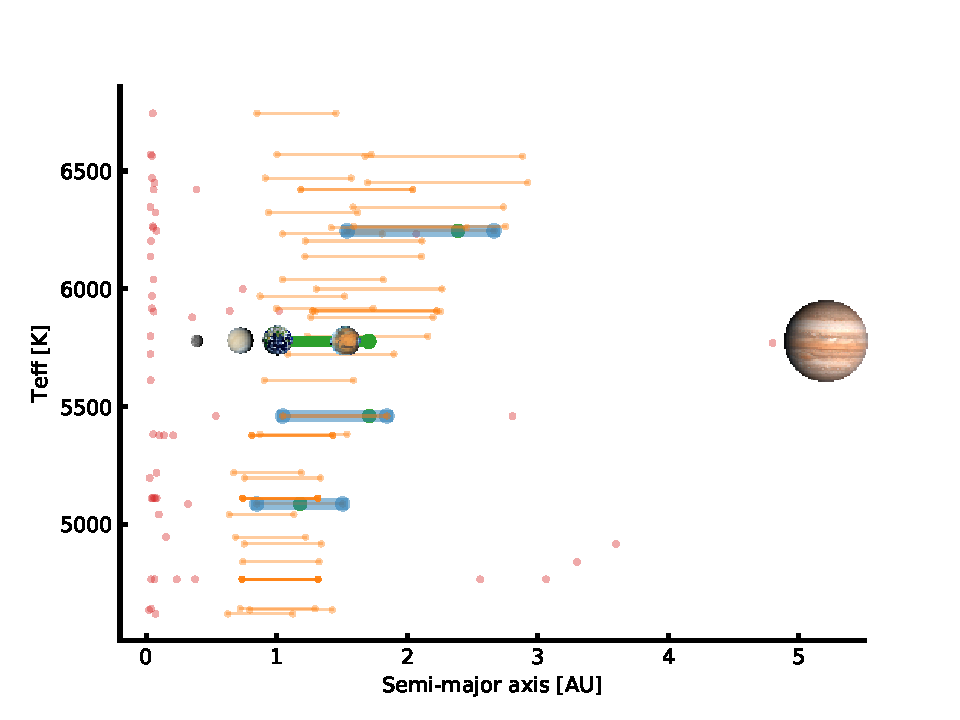
\includegraphics[width=0.8\linewidth]{figures/HZ.pdf}
    \caption{The habitable zone for the updated SWEET-Cat stars. The coloured line shows the
             theoretical habitable zone, while the dots shows the location of the planets in the
             actual system. The blue lines show the habitable zone of the three stars where a planet
             is located within it (green points). The red dots and orange lines are systems which
             does not lie within the habitable zone.}
    \label{fig:HZ}
\end{figure}



\subsection{Changes to planetary parameters}

As a results to the analysis above, it is expected that some planetary parameters will change
compared with the previous literature values.

Therefore the radius and mass of all the 50 new stars updated in SWEET-Cat were computed using the
empirical formula presented in \citet{Torres2010}. Some of the stars have radii derived from
different methods, usually from isochrones. These radii generally show a good correlation with radii
derived from \citet{Torres2010} if the literature parameters of $T_\mathrm{eff}$, $\log g$, and
$[\ion{Fe}/\ion{H}]$ are used. However, when comparing with the new radius derived using the
parameters presented here, the results can differ by up to 65\%. This is shown in \fref{fig:RR} how
the radius calculated from \citet{Torres2010} differs between the literature atmospheric parameters
and the new homogeneous atmospheric parameters presented here. Note that stellar radii are provided
by many of the authors from different discovery papers, but here the atmospheric parameters via the
derivation of the stellar radius, as described above, are compared, rather than comparing the
stellar radii from different methods.

\begin{figure}[tpb]
    \centering
    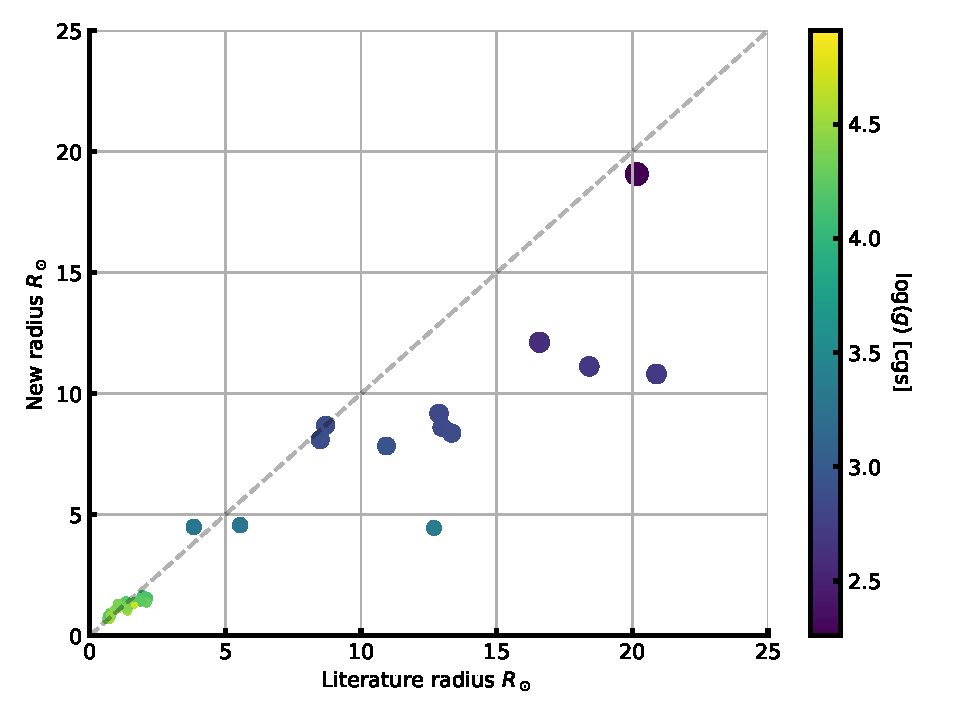
\includegraphics[width=0.8\linewidth]{figures/radiusVSradius.pdf}
    \caption{Stellar radius on both axes calculated based on \citet{Torres2010}. The x-axis shows
             the stellar radius based on the atmospheric parameters from the literature, while the
             y-axis indicates the new homogeneous parameters presented here. The colour and size
             indicate the surface gravity. This clearly shows that the disagreement is biggest for
             more evolved stars.}
    \label{fig:RR}
\end{figure}

In the sections below there follow a discussion of the systems (seven stars, eight exoplanets) where
the radius or mass of the stars changes more than 25\% and how this influences the planetary
parameters. The changes in radius for a star is primarily due to changes in $\log g$, which can be
used as an indicator of the evolutionary stage of a star.

The planetary radius, mass, and semi-major axis were re-derived when possible following the three
simple scaling relations based on Newton's law of gravity \citep{Newton1687} for deriving mass and
distance and simple geometry for radius \citep[see e.g.][]{Torres2008}
\begin{align}
    M_\mathrm{pl,new} &= \left(\frac{M_\mathrm{\ast,lit}}{M_\mathrm{\ast,new}}\right)^{-2/3} M_\mathrm{pl,lit}  \\
    R_\mathrm{pl,new} &= \left(\frac{R_\mathrm{\ast,lit}}{R_\mathrm{\ast,new}}\right) R_\mathrm{pl,lit} \\
    a_\mathrm{pl,new} &= \left(\frac{M_\mathrm{\ast,lit}}{M_\mathrm{\ast,new}}\right)^{1/3} a_\mathrm{pl,lit},
\end{align}
where the subscript ``lit'' denotes the value from the literature used in the comparison, the
subscript ``new'' indicates the new computed values, the subscript ``pl'' is short for planet, and
the subscript ``$\ast$'' is short for star; $M$, $R$, and $a$ are mass, radius, and semi-major axis,
respectively. Note that for the literature values, the values reported directly from the literature
were used and not the derived radius and mass from \citet{Torres2010}. To identify outliers, the
radii and masses were compared when derived from \citet{Torres2010} since this is a measure of how
the atmospheric parameters have changed.


\subsubsection{HAT-P-46}
\label{sub:HAT-P-46}

HAT-P-46 has two known exoplanets according to \citet{Hartmann2014}. The outer planet HAT-P-46 c is
not transiting, hence the radius is not known for this planet. The results presented above for this
star come from UVES/VLT data with a S/N of 208. \citet{Hartmann2014} derived the following
spectroscopic parameters: $T_\mathrm{eff}=\SI{6120(100)}{K}$, $\log g=\SI{4.25(11)}{dex}$, and
$[\ion{Fe}/\ion{H}]=\SI{0.30(10)}{dex}$. Note that for this star the asteroseismic correction
applied (see \sref{sec:sweetcat_analysis}) results in a corrected $\log g$ below 4.2dex, so the
spectroscopic $\log g$ was used for this star.

If mass and radius is derived of HAT-P-46 b with the new parameters, the radius obtained is
$R_\mathrm{pl}=0.93R_J$, while \citet{Hartmann2014} derived $R_\mathrm{pl} = 1.28R_J$. No change in
mass is seen (\citealt{Hartmann2014} found $M_\mathrm{pl}=0.49M_J$); however, there is a decrease in
the radius, and this results with a more dense planet, $\rho_\mathrm{pl}=\SI{0.76}{g/cm^3}$ from
$\rho_\mathrm{pl}=\SI{0.28\pm0.10}{g/cm^3}$.

Only the minimum mass is known for the secondary companions, as it does not transit HAT-P-46 seen
from Earth. With the derived parameters here, the minimum mass is $M\sin i_\mathrm{pl} = 1.97M_J$,
where \citet{Hartmann2014} presented $M\sin i_\mathrm{pl} = 2.00M_J$, so a very small change, as
expected.


\subsubsection{HD 120084}
\label{sub:HD_120084}

The exoplanet orbiting this star with a period of \SI{2082}{days} and a quite eccentric orbit at
0.66 was discovered by \citet{Sato2013}. The atmospheric parameters were derived by
\citet{Takeda2008} using a similar method to that described here. The quality of the spectra they
analysed, however, were not as high as those used here. Using the HIDES spectrograph at the
\SI{188}{cm} reflector at NAOJ, \citet{Takeda2008} reported an average S/N for their sample of
100-300 objects at a resolving power of \num{67000}. The spectrum used here is from ESPaDOnS with a
resolving power of \num{81000}, and with a S/N for this star at 850. With the new parameters
obtained, there is a slight decrease in stellar mass for the star at $1.93M_\odot$ compared to
$2.39M_\odot$ obtained by \citet{Takeda2008}, hence the minimum planetary mass is also slightly
lower, from $m_\mathrm{pl}\sin i=4.5M_J$ to $m_\mathrm{pl}\sin i=3.9M_J$. The stellar radius
decrease by 28\%, from $9.12R_\odot$ to $7.81R_\odot$. Since there are no observations of the planet
transiting, the planetary radius has not been computed.


\subsubsection{HD 233604}
\label{sub:HD_233604}

HD 233604 b was discovered by \citet{Nowak2013}, while the stellar atmospheric parameters of the
star were derived by \citet{Zielinski2012}, who used the same method as described here using the HRS
spectrograph at HET with a resolving power of \num{60000} with a typical S/N at 200-250. For the
analysis presented here, a spectrum from the FIES spectrograph was used with a slightly higher
resolution at \num{67000}, and similar but also slightly higher S/N at 320 for this star.

This planet is in a very close orbit with a semi-major axis of $\sim 15R_\ast$ ($R_\ast$ is the
stellar radius) using the parameters from \citet{Nowak2013}. Using the updated parameters presented
in this paper the stellar mass increase slightly from $1.5M_\odot$ to $1.9M_\odot$, and a decrease
in stellar radius from $10.5R_\odot$ to $8.6R_\odot$. This increases the semi-major axis to $\sim
21R_\ast$. We note that the correct stellar radii are used to describe the semi-major axis in both
cases. The increase in stellar mass leads to an increase in the minimum planetary mass, from
$m_\mathrm{pl}\sin i=6.58M_J$ to $m_\mathrm{pl}\sin i=7.79M_J$.

Moreover, \citet{Nowak2013} found a high \ion{Li}{} abundance at
$A(\ion{Li}{})_\mathrm{LTE}=\SI{1.400\pm0.042}{dex}$ for this star and speculated that this star
might have engulfed a planet. A more likely explanation is that this star has not yet reached the
first dredge-up process \citep{Nowak2013}. In the analysis here a much lower value is found,
$A(\ion{Li}{})_\mathrm{LTE}=\SI{0.92}{dex}$, and hence the star is not believed to be \ion{Li}{}
rich. The \ion{Li}{} abundance found here is in excellent agreement with \citet{Adamow2014}. Even
applying a NLTE correction, as was done in \citet{Adamow2014} ($A(\ion{Li}{})_\mathrm{NLTE}=1.08$),
this star is not \ion{Li}{} rich.


\subsubsection{HD 5583}
\label{sub:HD_5583}

This exoplanet was discovered by \citet{Niedzielski2016} with an orbital period of \SI{139}{days}
around a K giant. This exoplanet was discovered with the radial velocity technique, and the
planetary radius is not known. The stellar parameters were derived in a similar manner to that
presented here \citep[see][and references therein]{Niedzielski2016}; the biggest disagreement is in
the surface gravity. Here was derived a $\log g$ that is higher by \SI{0.34}{dex}, which gives a
stellar radius that is smaller by 37\%. The derived mass is 15\% higher, which in turn increases the
minimum planetary mass from $m_\mathrm{pl}\sin i=5.78M_J$ to $m_\mathrm{pl}\sin i=8.63M_J$. Even
with the increase in mass, it is still within the planetary regime for most inclinations, as was
noted by \citet{Niedzielski2016}.



\subsubsection{HD 81688}
\label{sub:HD81688}

This exoplanet was discovered by \citet{Sato2008} with the RV method. The host star is a metal-poor
K giant. The atmospheric parameters presented in \citet{Sato2008} are obtained via the same method
as presented here, and the agreement is quite good. Once again the big disagreement is in the
surface gravity: Here was obtained \SI{0.48}{dex} higher. Even though the stellar atmospheric
parameters, and hence the planetary parameters, do change, the radius and mass derived are not far
from the values presented in the paper by \citet{Sato2008}. This is a case where the star was marked
as an outlier, due to the comparison between the radius and mass derived from \citet{Torres2010}.

The new stellar mass is the same as before, $2.1M_\odot$. The stellar radius changed from
$13.0R_\odot$ to $10.8R_\odot$. Since a transit of this star has not been observed and the stellar
mass remains the same, there is no change in the planetary parameters.

It is worth noting that this system is in an interesting configuration with a very close orbit
around an evolved star. This system, among others, has been the subject of work on planet engulfment
\citep[see e.g.][]{Kunitomo2011}.


\subsubsection{HIP 107773}
\label{sub:HIP_107773}

The planetary companion was presented in \citet{Jones2015} as an exoplanet around an
intermediate-mass evolved star. The stellar parameters were obtained from the analysis by
\citet{Jones2011} using the same method as presented here, but with a different line list, which
might lead to some disagreements. A higher $\log g$ (\SI{2.83}{dex} compared to \SI{2.60}{dex}) was
derived here, thus the star is slightly smaller with $11.6R_\odot$ to $9.2R_\odot$ and $2.4M_\odot$
to $2.1M_\odot$ for radius and mass of the star, respectively. The other atmospheric parameters are
very similar to those derived by \citet{Jones2011}. This leads to a reduced minimum mass of the
planetary companion from $m\sin i=1.98M_J$ to $m\sin i=1.78M_J$. The planetary radius has not been
measured.



\subsubsection{WASP-97}
\label{sub:WASP-97}

The exoplanet orbiting WASP-97 was discovered by \citet{Hellier2014}. The host star parameters were
derived using a similar method to that described here after co-adding several spectra from the
CORALIE spectrograph. They reach a S/N of 100 with a spectral resolution of \num{50000}. The
parameters presented here come from the UVES spectrograph with a S/N of more than 200.

The parameters do not change much for this planet. The minimum planetary mass changes from
$m_\mathrm{pl}\sin i=1.32M_J$ to $m_\mathrm{pl}\sin i=1.37M_J$ and the radius from $1.13R_J$ to
$1.42R_J$. This affects the density quite strongly; it changes from $\SI{1.13}{g/cm^3}$ to
$\SI{0.59}{g/cm^3}$. This exoplanet is then in the same category as Saturn; its density is lower
than water, but it is slightly larger than Jupiter.

\subsubsection{$\omega$ Serpentis (ome Ser)}
\label{sub:ome_Ser}

The exoplanet orbiting this star with a period of \SI{277}{days} and an eccentric orbit at 0.11 was
also presented by \citet{Sato2013}. The atmospheric parameters were derived in the same way as for
HD 120084. Data from FIES with a resolving power of \num{67000} was used, and with a S/N for this
star of 1168. With the new parameters a slightly higher stellar mass for the star is obtained at
$2.19M_\odot$ compared to the value of $2.17M_\odot$ obtained by \cite{Takeda2008}. This change is
not significant enough to change the minimum planetary mass at $m_\mathrm{pl}\sin i=1.7M_J$. The
stellar radius decreases by more than one solar radius, from $12.3R_\odot$ to $11.1R_\odot$.
However, since there are no observations of transiting exoplanets, any change in planetary radius
cannot be detected.



\subsubsection{o Ursa Major (omi UMa)}
\label{sub:omiUMa}

omi UMa b was discovered by \citet{Sato2012} using the RV method. The stellar parameters are from
\citet{Takeda2008}, as discussed above. The spectrum used for this star is from ESPaDOnS with a S/N
of more than 500 compared to the value of 100-300 reached for the large sample presented in
\citet{Takeda2008}. The luminosity and mass for omi UMa were obtained from theoretical evolutionary
tracks \citep[see][and references therein]{Sato2012}. The radius was then estimated using the
Stefan-Boltzmann relationship, using the measured luminosity and $T_\mathrm{eff}$.

The parameters presented here mainly differ in the surface gravity: here it is \SI{0.72}{dex} higher
at $\log g=3.36$. This leads to a big change in stellar mass and radius from $3.1M_\odot$ to
$1.6M_\odot$ and $14.1R_\odot$ to $4.5R_\odot$, respectively. \citet{Sato2012} have reported that
omi UMa b is the first planet candidate around a star more massive than $3M_\odot$, which is not
supported by the results presented here. With these updated results, the minimum mass of the planet
is now $m\sin i=2.7M_J$, whereas previously it was $m\sin i=4.1M_J$ \citep{Sato2012}. The exoplanet
is not reported to transit, as seen from Earth, so the radius for this exoplanet is not known, which
would have changed a great deal with these new results.




\section{Discovering two giant planet populations}


SWEET-Cat was recently combined with planetary masses to see two distinctive populations for giant
planets by \citet{Santos2017}. This can be seen in the mass histogram in \fref{fig:giantpopulations}
for the full sample of giant planets, with masses higher than 1 Jupiter mass and lower than 20
Jupiter masses, and for a sample constrained by: $\SI{4000}{K}\leq T_\mathrm{eff} \leq\SI{6500}{K}$
in order to have reliably atmospheric parameters from spectroscopic data, orbital periods above
\SI{10}{days} to avoid hot jupiters whose formation and migration process is debated \citep[see
e.g.]{Ngo2016}, orbital periods below 5 years to allow for the sample to be reasonable complete.
Last only stars brighter than 13 magnitude were included to ensure that the planetary masses can
have been derived with reasonable confidence using the radial velocities.

\begin{figure}[htpb!]
    \centering
    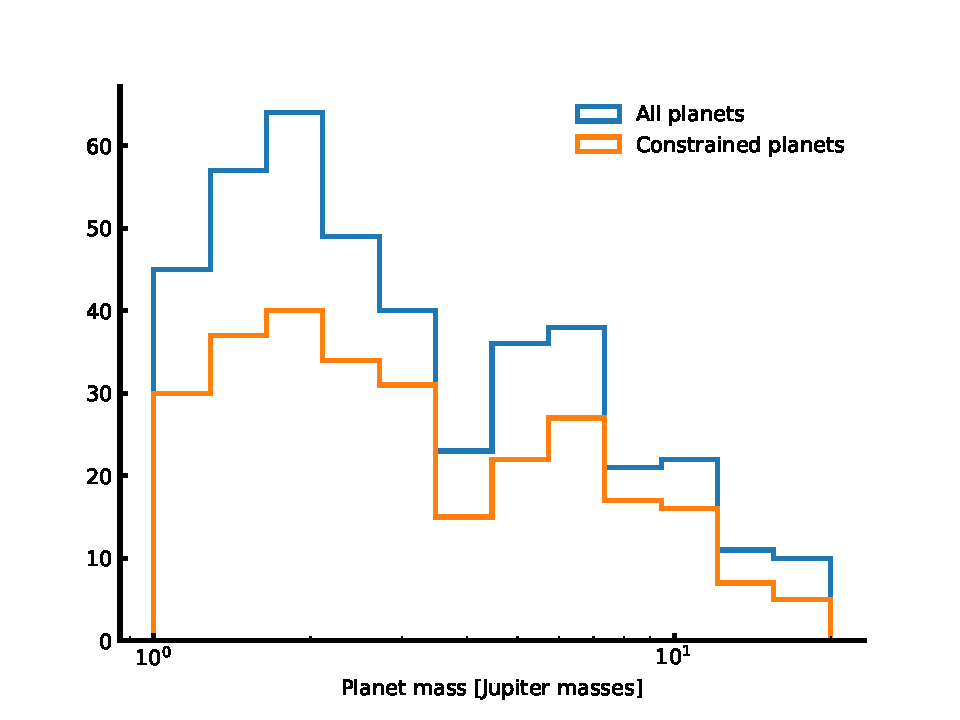
\includegraphics[width=1.0\linewidth]{figures/giantPopulation.pdf}
    \caption{Giant planet masses for the full sample and constrained sample (see text for details).
             This study was performed by \citet{Santos2017} to distinct two giant planet populations.}
    \label{fig:giantpopulations}
\end{figure}

By separating the distribution into two at $4M_{Jup}$, it can be shown \citep[see][for
details]{Santos2017} that the stars hosting the more massive giant planets are in average more
metal-poor compared to the stars hosting the lower mass giant planets. This suggest two different
stellar populations forming giant planets.


\section{Future work}

%!TEX root = thesis.tex
\chapter{Conclusions and future work}
\label{cha:future}

\section{Conclusions}

This thesis consisted of two separated analysis. 1) The analysis of NIR stellar spectra and the
compilation of a new iron line list for determining stellar atmospheric parameters, and 2) the
analysis of 50 planet-hosting stars and update of SWEET-Cat. These two different analyses (NIR and
optical) were both done using the same method; determination of stellar atmospheric parameters using
high quality spectra by imposing ionization and excitation equilibrium. In a few summarised points,
this thesis brings:

\begin{itemize}
  \item A new NIR line list consisting of 84 \ion{Fe}{I} lines and 5 \ion{Fe}{II} lines. This line
        list is optimised for usage with high quality spectra. The goal is to analyse FGK stars and
        making the bridge towards the M stars. Especially are the dwarf stars of most interest, in
        the context of exoplanets and the search of habitable worlds. ``Know the star, know the
        exoplanet'' is the key.

        The line list has been tested on few NIR spectra, mostly due to the lack of spectra and the
        difficulties it is to currently obtain any NIR spectra. This is about to change in the
        near future. The tests performed have been increasingly successful, and progress is evident.
  \item To analyse the data a new tool was created, \code{FASMA}. This tool provides many different
        options, can be used with different atmosphere models, is available to the community as a
        web application, and provides three different drivers for analysis of spectra: EW
        measurements, deriving parameters, and deriving abundances of a range of elements. A fourth
        driver is under construction which is to derive parameters using the synthesis method
        \citep{Tsantaki2017}.
  \item The analysis of 50 planet-host stars to increase the number of homogeneously analysed stars
        was also the first appearance and official usage of \code{FASMA}. This analysis increased
        the completeness to 85\% for stars brighter than 10 V magnitude. It is time consuming to
        obtain high quality spectra for stars fainter than this magnitude, however the completeness
        is still at 77\% for stars brighter than 12 V magnitude. Out of the 50 planet host stars
        analysed, eight changed either the radius or mass by more than 25\%. These eight systems
        were carefully analysed, and the updated planetary parameters (radius, mass, and density)
        were derived when possible.
\end{itemize}


\section{Future work}

While the tests with the NIR line list has been successful, there will still be room for
improvements. The same is the case for the \code{FASMA} and SWEET-Cat. Here are some of the main
points for (possible) future work.

\begin{itemize}
  \item The $\log g$ problem
  \item The model atmosphere used is reliable in the Porto group, however newer versions are
        available. It would be interesting to use more recent versions of the ATLAS9 atmosphere
        models, and to explorer other atmosphere models altogether, as the PHOENIX library.
  \item While \code{FASMA} is in a state where it work well and is stable, there are still ways to
        improve it. One way is to use machine learning to get a better guess of initial parameters.
        This work has already been initiated, and details on this can be seen in \cref{cha:fasmaML},
        however the work is not yet connected to \code{FASMA}.\unfinished{Write about non-LTE here?}
  \item After obtaining stellar atmospheric parameters from a high quality spectrum it is natural to
        explorer the spectrum with another purpose: to obtain abundances for other elements. The
        individual abundances of other elements than iron might be used to explorer the history of
        the star, and can be used in connection with the plant-star correlations. This is something
        that is already explored in detail in the optical, but is yet a relative new approach in the
        NIR from high quality spectra.
  \item One of the main limitations during this thesis have been the limited access to data. This
        lead to the analysis of synthetic spectra. It will be very interesting to explorer real data
        in the future. Particular interesting is the CARMENES library which is under constructions.
        This library will contain a high S/N spectrum of all the stars observed by CARMENES. This
        can be used to accurately explorer different part of the parameter space and find weak
        points in the methodology presented here in this thesis.
  \item This was already discussed previously, however, it will be interesting to update SWEET-Cat.
        These updates can include more columns such as abundances of the planet host, modelled mass,
        radius, and age, rotational velocity, etc. The update to SWEET-Cat can also be for the web
        interface. A wish is to update this and include easy-plotting capabilities for users to
        quickly explorer planet-star correlations.
\end{itemize}



\appendix

%!TEX root = thesis.tex
\chapter{NIR line list}
\label{cha:linelist}

\begin{longtable}{rrrrlr}
    \caption{\label{tab:nirll} The NIR iron line list. The $\log g$ are calibrated with \code{FASMA}
             using the ATLAS9 model atmospheres by \citet{Kurucz1993}.}\\
    \hline\hline
    Wavelength  & Atomic number & Excitation potential & $\log \mathit{gf}$ &  Element     &  Solar EW  \\[-0.3em]
      \AA{}     &               &  \si{eV}             &                    &              &  m\AA{}    \\
    \hline
    \endfirsthead
    \caption{continued.}\\
    \hline\hline
    Wavelength  & Atomic number & Excitation potential & $\log \mathit{gf}$ &  Element     &  Solar EW  \\[-0.3em]
      \AA{}     &               &  \si{eV}             &                    &              &  m\AA{}    \\
    \hline
    \endhead
    \hline
    \endfoot
      10065.05  &      26.0     &          4.83        &      -0.279        &  \ion{Fe}{I} &    94.0    \\
      10080.42  &      26.0     &          5.10        &      -1.964        &  \ion{Fe}{I} &     5.9    \\
      10081.39  &      26.0     &          2.42        &      -4.512        &  \ion{Fe}{I} &     6.9    \\
      10086.24  &      26.0     &          2.95        &      -3.978        &  \ion{Fe}{I} &     7.0    \\
      10137.10  &      26.0     &          5.09        &      -1.736        &  \ion{Fe}{I} &     9.8    \\
      10142.84  &      26.0     &          5.06        &      -1.554        &  \ion{Fe}{I} &    14.9    \\
      10145.56  &      26.0     &          4.80        &      -0.118        &  \ion{Fe}{I} &   109.0    \\
      10155.16  &      26.0     &          2.18        &      -4.336        &  \ion{Fe}{I} &    16.2    \\
      10156.51  &      26.0     &          4.59        &      -2.109        &  \ion{Fe}{I} &    12.2    \\
      10167.47  &      26.0     &          2.20        &      -2.319        &  \ion{Fe}{I} &   125.7    \\
      10195.11  &      26.0     &          2.73        &      -3.608        &  \ion{Fe}{I} &    22.6    \\
      10216.31  &      26.0     &          4.73        &       0.047        &  \ion{Fe}{I} &   129.9    \\
      10218.41  &      26.0     &          3.07        &      -2.893        &  \ion{Fe}{I} &    40.9    \\
      10265.22  &      26.0     &          2.22        &      -4.648        &  \ion{Fe}{I} &     8.1    \\
      10307.45  &      26.0     &          4.59        &      -2.432        &  \ion{Fe}{I} &     6.4    \\
      10332.33  &      26.0     &          3.63        &      -3.131        &  \ion{Fe}{I} &    10.5    \\
      10340.89  &      26.0     &          2.20        &      -3.665        &  \ion{Fe}{I} &    46.6    \\
      10347.97  &      26.0     &          5.39        &      -0.717        &  \ion{Fe}{I} &    37.0    \\
      10353.81  &      26.0     &          5.39        &      -0.989        &  \ion{Fe}{I} &    24.2    \\
      10364.06  &      26.0     &          5.45        &      -1.100        &  \ion{Fe}{I} &    18.0    \\
      10379.00  &      26.0     &          2.22        &      -4.236        &  \ion{Fe}{I} &    18.7    \\
      10388.75  &      26.0     &          5.45        &      -1.471        &  \ion{Fe}{I} &     8.7    \\
      10395.80  &      26.0     &          2.18        &      -3.435        &  \ion{Fe}{I} &    61.3    \\
      10423.03  &      26.0     &          2.69        &      -3.658        &  \ion{Fe}{I} &    22.9    \\
      10423.74  &      26.0     &          3.07        &      -3.119        &  \ion{Fe}{I} &    29.9    \\
      10469.65  &      26.0     &          3.88        &      -1.277        &  \ion{Fe}{I} &    89.3    \\
      10532.24  &      26.0     &          3.93        &      -1.650        &  \ion{Fe}{I} &    64.4    \\
      10555.65  &      26.0     &          5.45        &      -1.282        &  \ion{Fe}{I} &    13.1    \\
      10577.14  &      26.0     &          3.30        &      -3.222        &  \ion{Fe}{I} &    17.2    \\
      10616.72  &      26.0     &          3.27        &      -3.306        &  \ion{Fe}{I} &    15.6    \\
      10725.19  &      26.0     &          3.64        &      -2.948        &  \ion{Fe}{I} &    15.7    \\
      10753.00  &      26.0     &          3.96        &      -2.077        &  \ion{Fe}{I} &    39.7    \\
      10780.69  &      26.0     &          3.24        &      -3.553        &  \ion{Fe}{I} &    10.4    \\
      10783.05  &      26.0     &          3.11        &      -2.786        &  \ion{Fe}{I} &    47.0    \\
      10818.28  &      26.0     &          3.96        &      -2.160        &  \ion{Fe}{I} &    35.6    \\
      10863.52  &      26.0     &          4.73        &      -0.877        &  \ion{Fe}{I} &    67.1    \\
      10884.26  &      26.0     &          3.93        &      -2.129        &  \ion{Fe}{I} &    39.1    \\
      10896.30  &      26.0     &          3.07        &      -2.911        &  \ion{Fe}{I} &    42.9    \\
      11013.24  &      26.0     &          4.80        &      -1.240        &  \ion{Fe}{I} &    42.4    \\
      11026.79  &      26.0     &          3.94        &      -2.517        &  \ion{Fe}{I} &    21.2    \\
      11119.80  &      26.0     &          2.85        &      -2.452        &  \ion{Fe}{I} &    84.8    \\
      11641.80  &      26.0     &          4.58        &      -2.116        &  \ion{Fe}{I} &    15.6    \\
      11778.42  &      26.0     &          5.34        &      -1.708        &  \ion{Fe}{I} &     8.4    \\
      12053.08  &      26.0     &          4.56        &      -1.602        &  \ion{Fe}{I} &    41.3    \\
      12119.50  &      26.0     &          4.59        &      -1.897        &  \ion{Fe}{I} &    25.0    \\
      12213.34  &      26.0     &          4.64        &      -2.006        &  \ion{Fe}{I} &    19.1    \\
      12227.11  &      26.0     &          4.61        &      -1.408        &  \ion{Fe}{I} &    51.5    \\
      12244.92  &      26.0     &          3.64        &      -3.222        &  \ion{Fe}{I} &    11.8    \\
      12340.48  &      26.0     &          2.28        &      -4.680        &  \ion{Fe}{I} &     9.4    \\
      12342.92  &      26.0     &          4.64        &      -1.545        &  \ion{Fe}{I} &    42.1    \\
      12510.52  &      26.0     &          4.96        &      -1.930        &  \ion{Fe}{I} &    12.9    \\
      12557.00  &      26.0     &          2.28        &      -4.026        &  \ion{Fe}{I} &    33.8    \\
      12615.93  &      26.0     &          4.64        &      -1.686        &  \ion{Fe}{I} &    35.7    \\
      12638.70  &      26.0     &          4.56        &      -0.679        &  \ion{Fe}{I} &   112.3    \\
      12807.15  &      26.0     &          3.64        &      -2.649        &  \ion{Fe}{I} &    37.1    \\
      12808.24  &      26.0     &          4.99        &      -1.811        &  \ion{Fe}{I} &    16.4    \\
      12824.86  &      26.0     &          3.02        &      -3.612        &  \ion{Fe}{I} &    20.1    \\
      12840.57  &      26.0     &          4.96        &      -1.612        &  \ion{Fe}{I} &    25.3    \\
      12879.77  &      26.0     &          2.28        &      -3.525        &  \ion{Fe}{I} &    68.7    \\
      12896.12  &      26.0     &          4.91        &      -1.713        &  \ion{Fe}{I} &    23.2    \\
      12933.01  &      26.0     &          5.02        &      -1.879        &  \ion{Fe}{I} &    13.9    \\
      12934.67  &      26.0     &          5.39        &      -1.103        &  \ion{Fe}{I} &    30.9    \\
      13014.84  &      26.0     &          5.45        &      -1.542        &  \ion{Fe}{I} &    12.3    \\
      13352.17  &      26.0     &          5.31        &      -0.355        &  \ion{Fe}{I} &    94.4    \\
      13392.10  &      26.0     &          5.35        &      -0.105        &  \ion{Fe}{I} &   115.1    \\
      15194.49  &      26.0     &          2.22        &      -4.808        &  \ion{Fe}{I} &    14.1    \\
      15201.57  &      26.0     &          5.49        &      -1.315        &  \ion{Fe}{I} &    29.0    \\
      15207.53  &      26.0     &          5.38        &       0.311        &  \ion{Fe}{I} &   215.9    \\
      15335.38  &      26.0     &          5.41        &       0.252        &  \ion{Fe}{I} &   205.2    \\
      15490.34  &      26.0     &          2.20        &      -4.787        &  \ion{Fe}{I} &    16.1    \\
      15593.74  &      26.0     &          5.03        &      -1.796        &  \ion{Fe}{I} &    28.0    \\
      15611.15  &      26.0     &          3.42        &      -2.966        &  \ion{Fe}{I} &    51.6    \\
      15631.95  &      26.0     &          5.35        &       0.171        &  \ion{Fe}{I} &   207.0    \\
      15648.51  &      26.0     &          5.43        &      -0.633        &  \ion{Fe}{I} &    93.8    \\
      15676.58  &      26.0     &          5.11        &      -1.848        &  \ion{Fe}{I} &    22.3    \\
      16198.50  &      26.0     &          5.41        &      -0.376        &  \ion{Fe}{I} &   131.4    \\
      17420.83  &      26.0     &          3.88        &      -3.628        &  \ion{Fe}{I} &     6.7    \\
      19923.34  &      26.0     &          5.02        &      -1.536        &  \ion{Fe}{I} &    49.7    \\
      21851.38  &      26.0     &          3.64        &      -3.578        &  \ion{Fe}{I} &    12.7    \\
      22257.11  &      26.0     &          5.06        &      -0.704        &  \ion{Fe}{I} &   132.5    \\
      22380.80  &      26.0     &          5.03        &      -0.377        &  \ion{Fe}{I} &   179.4    \\
      22392.88  &      26.0     &          5.10        &      -1.330        &  \ion{Fe}{I} &    60.8    \\
      22619.84  &      26.0     &          4.99        &      -0.564        &  \ion{Fe}{I} &   158.2    \\
      23308.48  &      26.0     &          4.08        &      -2.705        &  \ion{Fe}{I} &    31.3    \\
      10427.31  &      26.1     &          6.08        &      -1.575        & \ion{Fe}{II} &    13.7    \\
      10501.50  &      26.1     &          5.55        &      -1.861        & \ion{Fe}{II} &    19.5    \\
      10862.64  &      26.1     &          5.59        &      -2.006        & \ion{Fe}{II} &    15.3    \\
      11125.58  &      26.1     &          5.62        &      -2.213        & \ion{Fe}{II} &    10.5    \\
      13251.14  &      26.1     &          9.41        &       0.768        & \ion{Fe}{II} &    13.4    \\
\end{longtable}

\begin{landscape}
\chapter{SWEET-Cat update of 50 planet hosts}
\label{cha:SCtables}

\begin{ThreePartTable}
% \advance\vsize5cm
% \csname @colroom\endcsname=\vsize
\textheight=\vsize
\csname @colht\endcsname=\vsize
% \setlength\extrarowheight{4pt}
\hskip-4em  % push the table a bit to the left...
\begin{longtable}{lllrlclr}

\caption{\label{tab:SCresults}
         Derived parameters for the 50 stars in our sample. The S/N was measured by ARES.}\\

 \hline\hline
 Star  & $T_\mathrm{eff}$ & $\log g$ & $[\ion{Fe}/\ion{H}]$ &  $\xi_\mathrm{micro}$ &  $\xi_\mathrm{micro}$ fixed?  &  Instrument  &  S/N  \\[-0.3em]
       &       [K]        &  [cgs]   &                      &     [km/s]            &                               &              &       \\
 \hline
 \endfirsthead
 \caption{continued.}\\
 \hline\hline
 Star  & $T_\mathrm{eff}$ & $\log g$ & $[\ion{Fe}/\ion{H}]$ &  $\xi_\mathrm{micro}$ &  $\xi_\mathrm{micro}$ fixed?  &  Instrument  &  S/N  \\[-0.3em]
       &       [K]        &  [cgs]   &                      &     [km/s]            &                               &              &       \\
 \hline
 \endhead
 \hline
 \endfoot
 \endlastfoot
 \hline
      \object{BD -11 4672}    &   \num{4553(75)}    &  \num{4.87(51)}             &  \num{-0.30(02)}  &  \num{0.14(07)}  & yes  &  FIES             &  487  \\
      \object{BD +49  828}    &   \num{5015(36)}    &  \num{2.87(9)}\tnote{a}     &  \num{-0.01(03)}  &  \num{1.48(04)}  & no   &  FIES             &  567  \\
      \object{GJ 785}         &   \num{5087(48)}    &  \num{4.42(10)}             &  \num{-0.01(03)}  &  \num{0.69(10)}  & no   &  HARPS            &  801  \\
      \object{HATS-1}         &   \num{5969(46)}    &  \num{4.39(6)}              &  \num{-0.04(04)}  &  \num{1.06(08)}  & no   &  UVES             &  155  \\
      \object{HATS-5}         &   \num{5383(91)}    &  \num{4.41(22)}             &  \num{ 0.08(06)}  &  \num{0.91(14)}  & no   &  UVES             &  158  \\
      \object{HAT-P-12}       &   \num{4642(106)}   &  \num{4.53(27)}             &  \num{-0.26(06)}  &  \num{0.28(63)}  & no   &  FIES             &  185  \\
      \object{HAT-P-24}       &   \num{6470(181)}   &  \num{4.33(27)}             &  \num{-0.41(10)}  &  \num{1.40(03)}  & yes  &  UVES             &  158  \\
      \object{HAT-P-39}       &   \num{6745(236)}   &  \num{4.39(47)}             &  \num{-0.21(12)}  &  \num{1.53(04)}  & yes  &  UVES             &  127  \\
      \object{HAT-P-42}       &   \num{5903(66)}    &  \num{4.29(10)}\tnote{a}    &  \num{ 0.34(05)}  &  \num{1.19(08)}  & no   &  UVES             &  130  \\
      \object{HAT-P-46}       &   \num{6421(121)}   &  \num{4.53(14)}\tnote{a}    &  \num{ 0.16(09)}  &  \num{1.67(18)}  & no   &  UVES             &  208  \\[5pt]
      \object{HD 120084}      &   \num{4969(40)}    &  \num{2.94(14)}\tnote{a}    &  \num{ 0.12(03)}  &  \num{1.41(04)}  & no   &  ESPaDOnS         &  852  \\
      \object{HD 192263}      &   \num{4946(46)}    &  \num{4.61(14)}             &  \num{-0.05(02)}  &  \num{0.66(12)}  & no   &  HARPS            &  415  \\
      \object{HD 219134}      &   \num{4767(70)}    &  \num{4.57(17)}             &  \num{ 0.00(04)}  &  \num{0.59(24)}  & no   &  ESPaDOnS         &  725  \\
      \object{HD 220842}      &   \num{5999(39)}    &  \num{4.30(6)}\tnote{a}     &  \num{-0.08(03)}  &  \num{1.21(05)}  & no   &  FIES             &  459  \\
      \object{HD 233604}      &   \num{4954(46)}    &  \num{2.86(11)}\tnote{a}    &  \num{-0.14(04)}  &  \num{1.61(05)}  & no   &  FIES             &  314  \\
      \object{HD 283668}      &   \num{4841(73)}    &  \num{4.51(18)}             &  \num{-0.74(04)}  &  \num{0.16(61)}  & no   &  FIES             &  592  \\
      \object{HD 285507}      &   \num{4620(126)}   &  \num{4.72(61)}             &  \num{ 0.04(06)}  &  \num{0.74(43)}  & no   &  UVES             &  239  \\
      \object{HD 5583}        &   \num{4986(35)}    &  \num{2.87(9)}\tnote{a}     &  \num{-0.35(03)}  &  \num{1.62(04)}  & no   &  FIES             &  933  \\
      \object{HD 81688}       &   \num{4903(21)}    &  \num{2.70(5)}\tnote{a}     &  \num{-0.21(02)}  &  \num{1.54(02)}  & no   & \tnote{b}         & 1350, 860  \\
      \object{HD 82886}       &   \num{5123(18)}    &  \num{3.30(4)}\tnote{a}     &  \num{-0.25(01)}  &  \num{1.16(02)}  & no   & \tnote{c}         & 1198,1294  \\[5pt]
      \object{HD 87883}       &   \num{4917(68)}    &  \num{4.53(19)}             &  \num{ 0.02(03)}  &  \num{0.46(21)}  & no   &  ESPaDOnS         &  753  \\
      \object{HIP 107773}     &   \num{4957(49)}    &  \num{2.83(9)}\tnote{a}     &  \num{ 0.04(04)}  &  \num{1.49(05)}  & no   &  UVES             &  218  \\
      \object{HIP 11915}      &   \num{5770(14)}    &  \num{4.33(3)}              &  \num{-0.06(01)}  &  \num{0.95(02)}  & no   &  HARPS            &  709  \\
      \object{HIP 116454}     &   \num{5042(72)}    &  \num{4.69(15)}             &  \num{-0.16(03)}  &  \num{0.71(17)}  & no   &  UVES             &  412  \\
      \object{HR 228}         &   \num{5042(42)}    &  \num{3.30(9)}\tnote{a}     &  \num{ 0.07(03)}  &  \num{1.14(04)}  & no   &  UVES             &  400  \\
      \object{KELT-6}         &   \num{6246(88)}    &  \num{4.22(9)}\tnote{a}     &  \num{-0.22(06)}  &  \num{1.66(13)}  & no   &  FIES             &  374  \\
      \object{Kepler-37}      &   \num{5378(53)}    &  \num{4.47(12)}             &  \num{-0.23(04)}  &  \num{0.58(13)}  & no   &  FIES             &  205  \\
      \object{Kepler-444}     &   \num{5111(43)}    &  \num{4.50(13)}             &  \num{-0.51(03)}  &  \num{0.37(15)}  & no   &  FIES             &  675  \\
      \object{mu Leo}         &   \num{4605(94)}    &  \num{2.61(26)}\tnote{a}    &  \num{ 0.25(06)}  &  \num{1.64(11)}  & no   &  ESPaDOnS         &  354  \\[5pt]
      \object{ome Ser}        &   \num{4928(35)}    &  \num{2.69(6)}\tnote{a}     &  \num{-0.11(03)}  &  \num{1.55(04)}  & no   &  FIES             & 1168  \\
      \object{omi UMa}        &   \num{5499(52)}    &  \num{3.36(7)}\tnote{a}     &  \num{-0.01(05)}  &  \num{1.98(06)}  & no   &  ESPaDOnS         &  527  \\
      \object{Qatar-2}        &   \num{4637(316)}   &  \num{4.53(62)}             &  \num{ 0.09(17)}  &  \num{0.63(83)}  & no   &  UVES             &   97  \\
      \object{SAND364}        &   \num{4457(104)}   &  \num{2.26(20)}\tnote{a}    &  \num{-0.04(06)}  &  \num{1.60(11)}  & no   &  UVES             &  220  \\
      \object{TYC+1422-614-1} &   \num{4908(41)}    &  \num{2.90(12)}\tnote{a}    &  \num{-0.07(03)}  &  \num{1.57(05)}  & no   &  FIES             &  506  \\
      \object{WASP-37}        &   \num{5917(72)}    &  \num{4.25(15)}             &  \num{-0.23(05)}  &  \num{0.59(13)}  & no   &  FIES             &  232  \\
      \object{WASP-44}        &   \num{5612(80)}    &  \num{4.39(30)}             &  \num{ 0.17(06)}  &  \num{1.32(13)}  & no   &  UVES             &  125  \\
      \object{WASP-52}        &   \num{5197(83)}    &  \num{4.55(30)}             &  \num{ 0.15(05)}  &  \num{1.16(14)}  & no   &  UVES             &  125  \\
      \object{WASP-58}        &   \num{6039(55)}    &  \num{4.23(10)}             &  \num{-0.09(04)}  &  \num{1.12(08)}  & no   &  FIES             &  310  \\
      \object{WASP-61}        &   \num{6265(168)}   &  \num{4.21(21)}\tnote{a}    &  \num{-0.38(11)}  &  \num{1.44(02)}  & yes  &  UVES             &  163  \\[5pt]
      \object{WASP-72}        &   \num{6570(85)}    &  \num{4.25(13)}             &  \num{ 0.15(06)}  &  \num{2.30(15)}  & no   &  UVES             &  174  \\
      \object{WASP-73}        &   \num{6203(32)}    &  \num{4.16(6)}\tnote{a}     &  \num{ 0.20(02)}  &  \num{1.66(04)}  & np   & \tnote{d}         & 193,231 \\
      \object{WASP-75}        &   \num{6203(46)}    &  \num{4.42(22)}\tnote{a}    &  \num{ 0.24(03)}  &  \num{1.45(06)}  & no   &  UVES             &  189  \\
      \object{WASP-76}        &   \num{6347(52)}    &  \num{4.29(8)}\tnote{a}     &  \num{ 0.36(04)}  &  \num{1.73(06)}  & no   &  UVES             &  165  \\
      \object{WASP-82}        &   \num{6563(55)}    &  \num{4.29(10)}\tnote{a}    &  \num{ 0.18(04)}  &  \num{1.93(08)}  & no   &  UVES             &  239  \\
      \object{WASP-88}        &   \num{6450(61)}    &  \num{4.24(6)}\tnote{a}     &  \num{ 0.03(04)}  &  \num{1.79(09)}  & no   &  UVES             &  174  \\
      \object{WASP-94 A}      &   \num{6259(34)}    &  \num{4.34(7)}\tnote{a}     &  \num{ 0.35(03)}  &  \num{1.50(04)}  & no   &  UVES             &  356  \\
      \object{WASP-94 B}      &   \num{6137(21)}    &  \num{4.42(5)}\tnote{a}     &  \num{ 0.33(02)}  &  \num{1.29(03)}  & no   &  UVES             &  397  \\
      \object{WASP-95}        &   \num{5799(31)}    &  \num{4.29(5)}\tnote{a}     &  \num{ 0.22(03)}  &  \num{1.18(04)}  & no   &  UVES             &  247  \\
      \object{WASP-97}        &   \num{5723(52)}    &  \num{4.24(7)}              &  \num{ 0.31(04)}  &  \num{1.03(08)}  & no   &  UVES             &  219  \\[5pt]
      \object{WASP-99}        &   \num{6324(89)}    &  \num{4.34(12)}             &  \num{ 0.27(06)}  &  \num{1.83(12)}  & no   &  UVES             &  249  \\
      \object{WASP-100}       &   \num{6853(209)}   &  \num{4.15(26)}\tnote{a}    &  \num{-0.30(12)}  &  \num{1.87(02)}  & yes  &  UVES             &  166  \\
  \hline
\end{longtable}
  \begin{tablenotes}
    \item [a] Spectroscopic $\log g$.
    \item [b] Weighted average of ESPaDoNS and FIES results.
              The parameters are (FIES in parantheses):
              $T_\mathrm{eff}=4870(4934)\pm30(29)$,
              $\log g=2.50(2.73)\pm0.14(0.05)$,
              $[\ion{Fe}/\ion{H}]=-0.26(-0.19)\pm0.03(0.02)$, and
              $\xi_\mathrm{micro}=1.50(1.59)\pm0.03(0.03)$.
    \item [c] Weighted average of ESPaDoNS and FIES results.
              The parameters are (FIES in parantheses):
              $T_\mathrm{eff}=5124(5121)\pm22(29)$,
              $\log g=3.30(3.31)\pm0.05(0.07)$,
              $[\ion{Fe}/\ion{H}]=-0.25(-0.24)\pm0.02(0.02)$, and
              $\xi_\mathrm{micro}=1.15(1.17)\pm0.03(0.04)$.
    \item [d] Weighted average of UVES and FEROS results.
              The parameters are (FEROS in parantheses):
              $T_\mathrm{eff}=6313(6162)\pm61(37)$,
              $\log g=4.26(4.14)\pm0.15(0.06)$,
              $[\ion{Fe}/\ion{H}]=0.22(0.19)\pm0.04(0.03)$, and
              $\xi_\mathrm{micro}=1.85(1.61)\pm0.08(0.04)$.
  \end{tablenotes}
\end{ThreePartTable}

\clearpage
\begin{longtable}{lllrll}
    \caption{\label{tab:oldSC} Previous parameters from SWEET-Cat.}\\
    \hline\hline
    Star  & $T_\mathrm{eff}$ & $\log g$ & $[\ion{Fe}/\ion{H}]$ &  $\xi_\mathrm{micro}$ &  Reference  \\[-0.3em]
          &       [K]        &  [cgs]   &                      &     [km/s]            &             \\
    \hline
    \endfirsthead
    \caption{continued.}\\
    \hline\hline
    Star  & $T_\mathrm{eff}$ & $\log g$ & $[\ion{Fe}/\ion{H}]$ &  $\xi_\mathrm{micro}$ &  Reference  \\[-0.3em]
          &       [K]        &  [cgs]   &                      &     [km/s]            &             \\
    \hline
    \endhead
    \hline
    \endfoot
    \object{BD-114672}       &    $4475 \pm 100$   &    $4.10 \pm 0.36$   &    $-0.48 \pm 0.05$   &    $0.67 \pm 0.16$   &    \citet{Moutou2015}       \\
    \object{BD +49 828}      &    $4943 \pm  30$   &    $2.85 \pm 0.09$   &    $-0.19 \pm 0.06$   &          ...         &    \citet{Niedzielski2015}  \\
    \object{GJ 785}          &    $5144 \pm  50$   &    $4.60 \pm 0.06$   &    $ 0.08 \pm 0.03$   &          ...         &    \citet{Howard2011}       \\
    \object{HATS-1}          &    $5780 \pm 100$   &    $4.40 \pm 0.08$   &    $-0.06 \pm 0.12$   &          ...         &    \citet{Penev2013}        \\
    \object{HATS-5}          &    $5304 \pm  50$   &    $4.53 \pm 0.02$   &    $ 0.19 \pm 0.08$   &          ...         &    \citet{Zhou2014}         \\
    \object{HAT-P-12}        &    $4650 \pm  60$   &    $4.61 \pm 0.02$   &    $-0.29 \pm 0.05$   &          ...         &    \citet{Lee2014}          \\
    \object{HAT-P-24}        &    $6373 \pm  80$   &    $4.29 \pm 0.04$   &    $-0.16 \pm 0.08$   &          ...         &    \citet{Kipping2010}      \\
    \object{HAT-P-39}        &    $6340 \pm 100$   &    $4.16 \pm 0.03$   &    $ 0.19 \pm 0.10$   &          ...         &    \citet{Hartman2012}      \\
    \object{HAT-P-46}        &    $6120 \pm 100$   &    $4.25 \pm 0.11$   &    $ 0.30 \pm 0.10$   &    $0.85 \pm  ...$   &    \citet{Hartman2014}      \\
    \object{HAT-P-42}        &    $5743 \pm  50$   &    $4.14 \pm 0.07$   &    $ 0.27 \pm 0.08$   &          ...         &    \citet{Boisse2013}       \\
    \object{HD 120084}       &    $4892 \pm  22$   &    $2.71 \pm 0.08$   &    $ 0.09 \pm 0.05$   &    $1.31 \pm 0.10$   &    \citet{Sato2013}         \\
    \object{HD 192263}       &    $4906 \pm  57$   &    $4.36 \pm 0.17$   &    $-0.07 \pm 0.02$   &    $0.78 \pm 0.12$   &    \citet{Tsantaki2013}     \\
    \object{HD 219134}       &    $4699 \pm  16$   &    $4.63 \pm 0.10$   &    $ 0.11 \pm 0.04$   &    $0.35 \pm 0.19$   &    \citet{Motalebi2015}     \\
    \object{HD 220074}       &    $3935 \pm 110$   &    $1.30 \pm 0.50$   &    $-0.25 \pm 0.25$   &    $1.60 \pm 0.30$   &    \citet{Lee2013}          \\
    \object{HD 220842}       &    $5920 \pm  20$   &    $4.24 \pm 0.02$   &    $-0.17 \pm 0.02$   &          ...         &    \citet{Hebrard2016}      \\
    \object{HD 233604}       &    $4791 \pm  45$   &    $2.55 \pm 0.18$   &    $-0.36 \pm 0.04$   &          ...         &    \citet{Nowak2013}        \\
    \object{HD 283668}       &    $4845 \pm  66$   &    $4.35 \pm 0.12$   &    $-0.75 \pm 0.12$   &    $0.02 \pm 0.30$   &    \citet{Wilson2016}       \\
    \object{HD 285507}       &    $4503 \pm  73$   &    $4.67 \pm 0.06$   &    $ 0.13 \pm 0.01$   &          ...         &    \citet{Quinn2014}        \\
    \object{HD 5583}         &    $4830 \pm  45$   &    $2.53 \pm 0.14$   &    $-0.50 \pm 0.18$   &          ...         &    \citet{Niedzielski2016}  \\
    \object{HD 81688}        &    $4753 \pm  15$   &    $2.22 \pm 0.05$   &    $-0.36 \pm 0.02$   &    $1.43 \pm 0.05$   &    \citet{Sato2008}         \\
    \object{HD 82886}        &    $5112 \pm  44$   &    $3.40 \pm 0.06$   &    $-0.31 \pm 0.03$   &          ...         &    \citet{Johnson2011}      \\
    \object{HD 87883}        &    $4958 \pm  44$   &    $4.56 \pm 0.06$   &    $ 0.07 \pm 0.03$   &          ...         &    \citet{Valenti2005}      \\
    \object{HIP 107773}      &    $4945 \pm 100$   &    $2.60 \pm 0.20$   &    $ 0.03 \pm 0.10$   &          ...         &    \citet{Jones2015}        \\
    \object{HIP 11915}       &    $5760 \pm   4$   &    $4.46 \pm 0.01$   &    $-0.06 \pm 0.00$   &          ...         &    \citet{Bedell2015}       \\
    \object{HIP 116454}      &    $5089 \pm  50$   &    $4.59 \pm 0.03$   &    $-0.16 \pm 0.08$   &          ...         &    \citet{Vanderburg2015}   \\
    \object{HR 228}          &    $4959 \pm  25$   &    $3.16 \pm 0.08$   &    $ 0.01 \pm 0.04$   &    $1.12 \pm 0.07$   &    \citet{Sato2013b}        \\
    \object{KELT-6}          &    $6102 \pm  43$   &    $4.07 \pm 0.06$   &    $-0.28 \pm 0.04$   &          ...         &    \citet{Collins2014}      \\
    \object{Kepler-37}       &    $5417 \pm  70$   &    $4.57 \pm 0.01$   &    $-0.32 \pm 0.07$   &          ...         &    \citet{Barclay2013}      \\
    \object{Kepler-444}      &    $5046 \pm  74$   &    $4.60 \pm 0.06$   &    $-0.55 \pm 0.07$   &          ...         &    \citet{Campante2015}     \\
    \object{mu Leo}          &    $4538 \pm  27$   &    $2.40 \pm 0.10$   &    $ 0.36 \pm 0.05$   &    $1.40 \pm 0.10$   &    \citet{Lee2014}          \\
    \object{ome Ser}         &    $4770 \pm  10$   &    $2.32 \pm 0.04$   &    $-0.24 \pm 0.02$   &    $1.34 \pm 0.04$   &    \citet{Sato2013}         \\
    \object{omi UMa}         &    $5242 \pm  10$   &    $2.64 \pm 0.03$   &    $-0.09 \pm 0.02$   &    $1.51 \pm 0.07$   &    \citet{Sato2012}         \\
    \object{Qatar-2}         &    $4645 \pm  50$   &    $4.60 \pm 0.02$   &    $-0.02 \pm 0.08$   &          ...         &    \citet{Bryan2012}        \\
    \object{SAND364}         &    $4284 \pm   9$   &    $2.20 \pm 0.06$   &    $-0.02 \pm 0.04$   &          ...         &    \citet{Brucalassi2014}   \\
    \object{TYC+1422-614-1}  &    $4806 \pm  45$   &    $2.85 \pm 0.18$   &    $-0.20 \pm 0.08$   &          ...         &    \citet{Niedzielski2015a} \\
    \object{WASP-37}         &    $5940 \pm  55$   &    $4.39 \pm 0.02$   &    $-0.40 \pm 0.12$   &          ...         &    \citet{Simpson2011}      \\
    \object{WASP-44}         &    $5400 \pm 150$   &    $4.48 \pm 0.07$   &    $ 0.06 \pm 0.10$   &          ...         &    \citet{Anderson2012}     \\
    \object{WASP-52}         &    $5000 \pm 100$   &    $4.58 \pm 0.01$   &    $ 0.03 \pm 0.12$   &          ...         &    \citet{Hebrard2013}      \\
    \object{WASP-58}         &    $5800 \pm 150$   &    $4.27 \pm 0.09$   &    $-0.45 \pm 0.09$   &          ...         &    \citet{Hebrard2013}      \\
    \object{WASP-61}         &    $6250 \pm 150$   &    $4.26 \pm 0.01$   &    $-0.10 \pm 0.12$   &          ...         &    \citet{Hellier2012}      \\
    \object{WASP-72}         &    $6250 \pm 100$   &    $4.08 \pm 0.13$   &    $-0.06 \pm 0.09$   &    $1.60 \pm 0.10$   &    \citet{Gillon2013}       \\
    \object{WASP-73}         &    $6030 \pm 120$   &    $3.92 \pm 0.08$   &    $ 0.14 \pm 0.14$   &    $1.10 \pm 0.20$   &    \citet{Delrez2014}       \\
    \object{WASP-75}         &    $6100 \pm 100$   &    $4.50 \pm 0.10$   &    $ 0.07 \pm 0.09$   &    $1.30 \pm 0.10$   &    \citet{Gomez2013}        \\
    \object{WASP-76}         &    $6250 \pm 100$   &    $4.13 \pm 0.02$   &    $ 0.23 \pm 0.10$   &    $1.40 \pm 0.10$   &    \citet{West2016}         \\
    \object{WASP-82}         &    $6490 \pm 100$   &    $3.97 \pm 0.02$   &    $ 0.12 \pm 0.11$   &    $1.50 \pm 0.10$   &    \citet{West2016}         \\
    \object{WASP-88}         &    $6430 \pm 130$   &    $4.03 \pm 0.09$   &    $-0.08 \pm 0.12$   &    $1.40 \pm 0.10$   &    \citet{Delrez2014}       \\
    \object{WASP-94 A}       &    $6170 \pm  80$   &    $4.27 \pm 0.07$   &    $ 0.26 \pm 0.15$   &          ...         &   \citet{Neveu2014}         \\
    \object{WASP-94 B}       &    $6040 \pm  90$   &    $4.26 \pm 0.06$   &    $ 0.23 \pm 0.14$   &          ...         &   \citet{Neveu2014}         \\
    \object{WASP-95}         &    $5630 \pm 130$   &    $4.38 \pm 0.03$   &    $ 0.14 \pm 0.16$   &          ...         &    \citet{Hellier2014}      \\
    \object{WASP-97}         &    $5640 \pm 100$   &    $4.43 \pm 0.03$   &    $ 0.23 \pm 0.11$   &          ...         &    \citet{Hellier2014}      \\
    \object{WASP-99}         &    $6180 \pm 100$   &    $4.12 \pm 0.03$   &    $ 0.21 \pm 0.15$   &          ...         &    \citet{Hellier2014}      \\
    \object{WASP-100}        &    $6900 \pm 120$   &    $4.04 \pm 0.11$   &    $-0.03 \pm 0.10$   &          ...         &    \citet{Hellier2014}      \\
\end{longtable}


\end{landscape}

%!TEX root = thesis.tex
\chapter{\code{FASMA} and machine learning}
\label{cha:fasmaML}

With the increasing amount of astrophysical data, it is important to perform a rapid and trustworthy
analysis. This is one of the strengths for \code{FASMA} when dealing with high quality spectroscopic
data for determination of stellar atmospheric parameters. Here a classic method to analyse these
large amount of data has been modernised with a new minimisation technique that utilise the physical
knowledge about the system. However smart it may sound like, it can be improved. The time consuming
part in \code{FASMA} are the calls to \code{MOOG}. In the end a couple of minutes are spent on the
minimisation on a modern computer.

This lead to a side-project: explorer the use of machine learning to determine stellar atmospheric
parameters. Machine learning (ML) is not a new topic in computer science, but it is a tool that is
steadily becoming more and more popular in today's science. The effort of using ML here is meant as
a proof of concept, and something that can be improved upon in the future.

The idea was to remove the expensive calls to \code{MOOG} completely. Two things are required in
order to do so in the approach presented here:
\begin{enumerate}
  \item Stellar atmospheric parameters of a large sample of stars with a big span in the parameter
        space
  \item The EW measurements of as many absorption lines as possible (in this case \ion{Fe}{I} and
        \ion{Fe}{II})
\end{enumerate}
Additionally it is here required that the above two points are obtained in a homogeneous way.
Luckily such a sample was already analysed during this thesis as a test of \code{FASMA} (see
\sref{sec:fasma_test}) where a sample of 582 stars were analysed; all of which meet the above
required criteria.

This data set of measurements of EWs and the parameters were organised and prepared in a big table
as follows:
\begin{itemize}
  \item Each row contains both the measurements of the EWs (first N columns) and the parameters
        (last four columns). The parameters are $T_\mathrm{eff}$, $\log g$, $[\ion{Fe}/\ion{H}]$,
        and $\xi_\mathrm{micro}$
  \item The columns excluding the last four are labelled with the wavelength of the absorption line
  \item All wavelength columns which contained at least one missing measurement of the EW for any
        of the 582 stars were removed
\end{itemize}
There are 58 wavelength columns after removing wavelength columns with missing measurements. Before
the removal there were 299 columns with wavelength. In this case the \code{scikit-learn}
package\footnote{\url{http://scikit-learn.org/}} from the Python ecosystem was used to train the
data set. This also package also include a tool to split the data into a training part and testing
part. This is particular useful when trying to evaluate the accuracy of the model used. Here the
training consist of 2/3 of the data, and the rest is for testing. This splitting is done randomly,
giving slight different results each time the script is executed.

The training itself is quite fast (less than \SI{10}{s}). However, the real power comes when the
trained model is saved to the disk, which can later be loaded again. In this way the training will
only be done once. Using the model to obtain the parameters is much less than \SI{1}{s}, which makes
is many orders of magnitudes faster\footnote{Improvements in the order of millions have been
obtained here.} than a more traditional approach as with \code{FASMA}.

When testing the model trained, the 1/3 data set is used to derive parameters. Those derived
parameters are then compared to the actual parameters with a mean absolute error. This gives an idea
of the accuracy. In \fref{fig:ml} the script was run 1000 times (the splitting was done randomly in
each run), and the error for each parameter is shown as a histogram. The mean errors for each
parameters are roughly $T_\mathrm{eff}:\SI{47}{K}$, $\log g:\SI{0.10}{dex}$,
$[\ion{Fe}/\ion{H}]:\SI{0.038}{dex}$, and $\xi_\mathrm{micro}:\SI{0.12}{km/s}$.

\begin{figure}[htpb!]
    \centering
    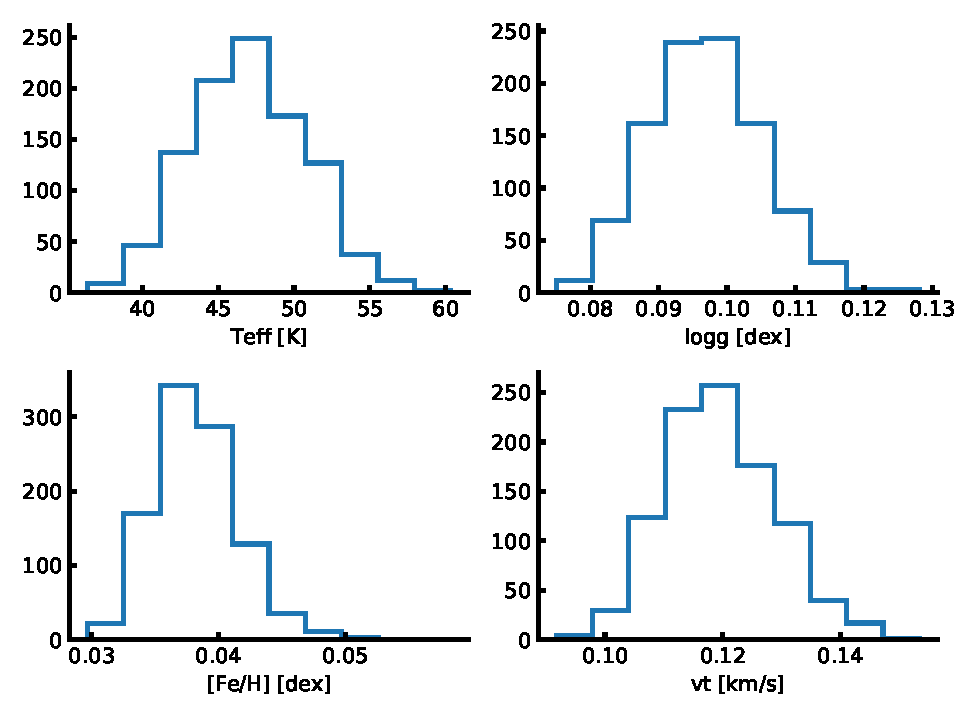
\includegraphics[width=1.0\linewidth]{figures/ML.pdf}
    \caption{Mean absolute error on each parameter after 1000 runs.}
    \label{fig:ml}
\end{figure}

There exists many different algorithms within \code{scikit-learn} to train the final model. In the
test here a simple \code{LinearRegression} was used. Other algorithms were tested as well, such as
\code{Ridge} and \code{Lasso}, however with very similar results. The main difference between the
different algorithms are found in the details on how the minimisation is done. This is described in
great detail in the online documentation.



%% This adds a line for the Bibliography in the Table of Contents.
\addcontentsline{toc}{chapter}{Bibliography}
% \bibliographystyle{plain}
%% *** Set the bibliography file. ***
\bibliography{thesis}
\bibliographystyle{astron}
\nocite{} %include everything.


\end{document}
